\documentclass[a4paper]{extarticle}
\usepackage[utf8]{inputenc}
\usepackage[italian]{babel}
\selectlanguage{italian}
\usepackage[table]{xcolor}
\usepackage{xcolor}
\usepackage{circuitikz}
\usetikzlibrary{positioning, circuits.logic.US}
\usetikzlibrary{shapes.geometric, arrows}
\usetikzlibrary {shapes.gates.logic.US, shapes.gates.logic.IEC, calc}
\tikzset {branch/.style={fill, shape = circle, minimum size = 3pt, inner sep = 0pt}}
\usetikzlibrary{matrix,calc}
\usepackage{multirow}
\usepackage{float}
\usepackage{geometry}
\usepackage{tabularx}
\usepackage{pgf-pie}
\usepackage{tikz}
\usepackage{amsmath}
\usepackage{amssymb}
\usepackage{color, soul}
\usepackage{fancyhdr}
\usepackage{graphicx}
\usepackage{subcaption}
\graphicspath{ {./img/} }
\newtheorem{theorem}{Teorema}[section]
\newtheorem{corollary}{Corollario}[theorem]
\newtheorem{lemma}[theorem]{Lemma}

% Specifiche
\geometry{
 a4paper,
 top=20mm,
 left=30mm,
 right=30mm,
 bottom=30mm
}

\nocite{*}
\graphicspath{ {./img/} }
\pagestyle{fancy}
\fancyhf{}
\fancyhead[LO]{\nouppercase{\leftmark}}
\fancyfoot[CE, CO]{\thepage}
\addtolength{\headheight}{1em}
\addtolength{\footskip}{-0.5em}

\newcommand{\quotes}[1]{``#1''}
\renewcommand\tabularxcolumn[1]{>{\vspace{\fill}}m{#1}<{\vspace{\fill}}}
\renewcommand\arraystretch{}
\newcolumntype{P}{>{\centering\arraybackslash}X}

\title{\textbf{Università di Trieste\\ \vspace{1em}
Laurea in ingegneria elettronica e informatica}}
\author{Enrico Piccin - Corso di Reti Logiche - Prof. Stefano Marsi}
\date{Anno Accademico 2022/2023 - 6 Ottobre 2022}

\begin{document}

\vspace{-10mm}
\maketitle

\tableofcontents
\newpage
\begin{center}
    6 Ottobre 2022
\end{center}

\vspace{1em}
\noindent
\section{Sistemi di numerazione e codici}
Di seguito si espone la definizione di \textbf{sistema di numerazione}:

% Tabella per le definizione di concetti, etc...
\vspace{1em}
\rowcolors{1}{black!5}{black!5}
\setlength{\tabcolsep}{14pt}
\renewcommand{\arraystretch}{2}
\noindent
\begin{tabularx}{\textwidth}{@{}|P|@{}}
    \hline
    {\textbf{SISTEMA DI NUMERAZIONE}}\\
    \parbox{\linewidth}{Un \textbf{sistema di numerazione} è un \textbf{insieme di simboli} (cifre) e regole, le quali consentono di associare ad una stringa di cifre il corrispondente valore numerico.\\
    I codici decimale, binario, ottale o esadecimale sono tutti codici posizionali, il cui valore dipende dalla posizione delle cifre.\vspace{3mm}}\\
    \hline
\end{tabularx}

\vspace{2em}
\noindent
\textbf{Osservazione}: La base $2$ è la più piccola possibile, in cui i bit sono associati agli stati ON/OFF.\\
Le basi 8 e 16, invece, permettono rappresentazioni più compatte del numero binari, soprattutto perché il passaggio da base 2 a base 8 o 16 e viceversa è particolarmente facile
\begin{align}
    55_10 & = 110111_2\\
    110111_2 & = 37_16 = 67_8
\end{align}

\vspace{1em}
\noindent
\subsection{Conversione tra basi diverse di numeri interi}
La conversione da base $10$ a base $2$, prevede di adottare il metodo delle \textbf{divisioni successive}: si divide ripetutamente il numero per la base voluta fino ad ottenere un quoziente nullo e si memorizzano i resti (la seq. dei resti ordinata rappresenta la notazione).\\
Per quanto detto, il passaggio da basi $B$ a $B^n$ e viceversa risulta particolarmente semplice:
\[157_10=10011101_2=235_8=9D_16\]

\vspace{1em}
\noindent
\textbf{Osservazione}: Si osservi che per convertire un numero da base $2$ a base $10$, non solo è possibile usare le potenze del due, ma è anche possibile partire dal bit più significativo e moltiplicarlo per $2$, sommarlo al bit successivo e moltiplicare per $2$, e via dicendo fino ad esaurire tutti i bit.

\vspace{1em}
\noindent
\subsection{Conversione tra basi diverse di numeri frazionari}
Com'è noto, la virgola distingue le cifre che vanno moltiplicate per la base $B$ con esponente positivo da quelle con esponente negativo, per cui
\[0.101 = 1 \cdot 2^{-1} + 0 \cdot 2^{-2} + 1 \cdot 2^{-3} = 0.5 + 0.125 = 0.625\]
Oppure si può anche traslare di $3$ posizioni la virgola (che in binario vuole dire moltiplicare per $2^3=8$) e convertire il numero binario come se fosse intero e poi dividerlo ancora per $2^3=8$, per cui
\[0.101 \hspace{1em} \rightarrow \hspace{1em} 0.101 \cdot 2^3 = 101 = 5 \hspace{1em} \rightarrow \hspace{1em} 0.101 = \frac{5}{2^3} = 0.625\]
Se, invece, bisogna passare da decimale a binario, si deve procedere per moltiplicazioni successive:
\[0.375_10 \hspace{1em} \rightarrow \hspace{1em} 0.375 \cdot 2 = 0.750 \hspace{1em} \rightarrow \hspace{1em} \textbf{0} + 0.750\]
\[0.750_10 \hspace{1em} \rightarrow \hspace{1em} 0.750 \cdot 2 = 1.500 \hspace{1em} \rightarrow \hspace{1em} \textbf{1} + 0.500\]
\[0.500_10 \hspace{1em} \rightarrow \hspace{1em} 0.500 \cdot 2 = 1.000 \hspace{1em} \rightarrow \hspace{1em} \textbf{1} + 0.000\]
Ecco, quindi, che il valore binario è stato ottenuto:
\[0.375_10 = 0.011_2\]

\vspace{1em}
\noindent
\textbf{Osservazione}: Ovviamente, è possibile che il processo sopra descritto cada in una ripetizione periodica. Allora, il processo di approssimazione può avvenire secondo due modalità:
\begin{enumerate}
    \item Per \textbf{troncamento}, in cui si lascia semplicemente il valore binario ottenuto così com'è;
    \item Per \textbf{arrotondamento}, in cui si considera il bit immediatamente successivo all'ultimo di quelli che si sta considerando e lo si somma all'ultima cifra, come mostrato di seguito:
    \[011011 \vert \boxed{1}01101 \rightarrow 011011+\boxed{1}=011100\]
\end{enumerate}
Non sorprende, poi, osservare che se con una base una notazione frazionaria richiede un numero finito di cifre, potrebbe richiederne infinite con una diversa notazione.

\vspace{1em}
\noindent
\subsection{Aritmetica binaria}
L'addizione binaria è molto semplice, mentre la sottrazione risulterebbe particolarmente ostica, a meno che non si considerasse la complementazione. Infatti, dovendo eseguire, in decimale, la differenza $123-73$, è sufficiente eseguire la somma $123+\text{comp}_{10}(73)$, in cui $\text{comp}_{10}(73)$ si calcola come segue

\vspace{1em}
\noindent
\begin{table}[H]
    \rowcolors{1}{white}{white}
\setlength{\tabcolsep}{4pt}
\renewcommand{\arraystretch}{1.2}
\centering
\begin{tabular}{cccc}
    9 & 9 & 9 & -\\
      & 7 & 3 & +\\
      &   & 1 & =\\
    \hline
    9 & 2 & 7
\end{tabular}
\end{table}
\vspace{1em}

\noindent
per cui si ottiene $123+\text{comp}_{10}(73)=123+927=1 \vert 050 \rightarrow 50$, eliminando l'$1$ del migliaio, in quanto aggiunto prima per la complementazione. Analogamente in binario.

\vspace{1em}
\noindent
\textbf{Osservazione}: Si osservi che, per ogni base $B$, esistono due complementi per un numero $N$:
\begin{itemize}
    \item Complemento a $B$, definito come $C_B = B^n-N$
    \item Complemento a $B-1$, definito come $C_{B-1}=B^n-1-N$
\end{itemize}
Non solo, ma dalla differenza di $N_1$ ed $N_2$, vi possono essere due casi:
\begin{itemize}
    \item $N_1 \geq N_2$: il risultato risulta maggiore o uguale a $B^n$, che pertanto va eliminato dal risultato finale (eliminazione dell'$1$ più significativo oltre il range del numero stesso)
    \item $N_1 < N_2$: il risultato risulta minore di $B^n$, e deve essere inteso come complemento a $B$ (pertanto rappresentante di un numero negativo) del risultato. Per conoscerne il valore assoluto, è necessario ri-complementarlo.
\end{itemize}
Si consideri, infatti, l'esempio seguente, in cui si esegue la differenza $21-46$, ovvero:

\vspace{1em}
\noindent
\begin{table}[H]
    \rowcolors{1}{white}{white}
\setlength{\tabcolsep}{4pt}
\renewcommand{\arraystretch}{1.2}
\centering
\begin{tabular}{ccccccc}
    0 & 1 & 0 & 1 & 0 & 1 & +\\
    0 & 1 & 0 & 0 & 1 & 0 & =\\
    \hline
    1 & 0 & 0 & 1 & 1 & 1
\end{tabular}
\end{table}
\vspace{1em}

\noindent
In cui non è stato ottenuto un $1$ nell'ultima operazione finale, pertanto il risultato $110111$ deve essere ulteriormente complementato, ottenendo $011001_2=25$, che è il valore assoluto della differenza.

\vspace{1em}
\noindent
\subsection{Rappresentazione dei numeri negativi}
I numeri negativi possono pertanto essere rappresentati in base al loro complemento a $B$. In base $B=10$, ciò non risulta essere usuale, ma si preferisce impiegare un segno grafico $-$.\\
In binario, ciò non risulta essere possibile, in cui i numeri negativi vengono rappresentati in base al loro complemento a $2$, usando il bit più significativo viene impiegato come \textbf{bit di segno}:
\[\colorbox{red}{1}\colorbox{cyan}{0}\colorbox{cyan}{1}\colorbox{cyan}{1}\colorbox{cyan}{1}\]
in cui la convenzione sul bit di segno è
\begin{itemize}
    \item \textbf{0}: numero positivo
    \item \textbf{1}: numero negativo
\end{itemize}
Attenzione che, eliminato il bit di segno in un numero binario
\begin{itemize}
    \item nel caso di un numero positivo (quindi avendo eliminato il bit $0$), i restanti numeri rappresentano il numero stesso:
    \[01001_2=+9_{10}\]
    \item nel caso di un numero negativo (quindi avendo eliminato il bit $1$), i restanti numeri rappresentano il numero complementato:
    \[11001_2=-C_2(1001)=-0111_2=-7_{10}\]
\end{itemize}

\vspace{1em}
\noindent
\subsection{Errori nei risultati}
Il risultato di un'operazione somma/sottrazione è coerente solo se il risultato non esce dal range dei numeri rappresentabili, per cui
\begin{itemize}
    \item il risultato è \textbf{corretto} se
    \begin{itemize}
        \item non si è avuto alcun riporto, nè nel bit di segno nè fuori dalla parola;
        \item si sono avuti riporti in entrambi;
    \end{itemize}
    \item il risultato è \textbf{errato} se si è avuto un solo riporto, o sul segno, o fuori dalla parola;
\end{itemize}
Dal punto di vista circuitale, per determinare se si è ottenuto un risultato corretto o meno, sarà sufficiente considerare il bit di riporto sul segno e quello fuori dalla parola e porli in XOR: se lo XOR produce come uscita $1$, allora si è verificato un errore, altrimenti il risultato è corretto.

\newpage
\begin{center}
    7 Ottobre 2022
\end{center}
Non deve sorprendere che un numero in una base non risulta essere periodico, mentre in altre basi esso lo è, in quanto le frazioni a disposizione sono differenti a seconda della base stessa; per esempio, le frazioni a disposizione per la base $3$ sono
\[3^{-1}=\frac{1}{3}, 3^{-2}=\frac{1}{9}, 3^{-3}=\frac{1}{27}\]\\
ed ecco che quindi $\frac{1}{3}$, in base $3$, si rappresenta come $0,1_3$.\\
Inoltre, se si adotta una notazione \textbf{unsigned} su $n$ bit, i possibili numeri rappresentabili sono $2^n$, da $0$ a $2^{n}-1$. Invece, se si adotta una notazione \textbf{signed} su $n$ bit, i numeri rappresentabili sono i valori da $0$ a $2^{n-1}-1$, e da $-1$ a $-2^{n-1}$; tuttavia l'intervallo è il medesimo.\\
Nella tabella seguente si espongono i valori interi \textbf{signed} su $4$ bit e i corrispondenti valori decimali se si considera la notazione con la virgola \textbf{signed} su $4$ bit (utilizzando $2$ bit dopo la virgola), ottenendo lo schema seguente:

% Tabella per le definizione di concetti, etc...
\vspace{1em}
\rowcolors{1}{white}{white}
\setlength{\tabcolsep}{4pt}
\renewcommand{\arraystretch}{1}
\begin{table}[H]
    \centering
    \begin{tabular}{c|cccc|c}
        Intero & & & & & Virgola\\
        \hline
        7 & 0 & 1 & 1 & 1 & 1.75\\
        6 & 0 & 1 & 1 & 0 & 1.50\\
        5 & 0 & 1 & 0 & 1 & 1.25\\
        4 & 0 & 1 & 0 & 0 & 1.00\\
        3 & 0 & 0 & 1 & 1 & 0.75\\
        2 & 0 & 0 & 1 & 0 & 0.50\\
        1 & 0 & 0 & 0 & 1 & 0.25\\
        0 & 0 & 0 & 0 & 0 & 0.00\\
        \hline
        -1 & 1 & 1 & 1 & 1 & -0.25\\
        -2 & 1 & 1 & 1 & 0 & -0.50\\
        -3 & 1 & 1 & 0 & 1 & -0.75\\
        -4 & 1 & 1 & 0 & 0 & -1.00\\
        -5 & 1 & 0 & 1 & 1 & -1.25\\
        -6 & 1 & 0 & 1 & 0 & -1.50\\
        -7 & 1 & 0 & 0 & 1 & -1.75\\
        -8 & 1 & 0 & 0 & 0 & -2.00\\
        \hline
    \end{tabular}
\end{table}

\vspace{1em}
\noindent
\subsection{Moltiplicazione e Divisione}
La moltiplicazione binaria è molto semplice, e segue la regola seguente:
\begin{itemize}
    \item $0 \cdot 0 = 0$
    \item $1 \cdot 0 = 0$
    \item $0 \cdot 1 = 0$
    \item $1 \cdot 1 = 1$
\end{itemize}
e si basa sull'automatismo dello \textbf{shift \& add}, come mostrato nel seguito:

% Tabella per le definizione di concetti, etc...
\vspace{1em}
\rowcolors{1}{white}{white}
\setlength{\tabcolsep}{4pt}
\renewcommand{\arraystretch}{1}
\begin{table}[H]
    \centering
    \begin{tabular}{ccccc}
          & 1 & 1 & 0 & $\times$\\
          &   & 1 & 0 & $=$\\
        \hline
          & 0 & 0 & 0 & $+$\\
        1 & 1 & 0 &   & $=$\\
        \hline
        1 & 1 & 0 & 0 &
    \end{tabular}
\end{table}

\noindent
e la divisione viene eseguita, di solito, per sottrazioni successive, particolarmente semplice da meccanizzare tramite automatismi informatici.

\vspace{1em}
\subsection{Casting}
Quando si considera un numero binario, risulta fondamentale capire se il valore risulta essere unsigned oppure signed; la differenza è fondamentale perché i due valori

% Tabella per le definizione di concetti, etc...
\vspace{1em}
\rowcolors{1}{white}{white}
\setlength{\tabcolsep}{4pt}
\renewcommand{\arraystretch}{1}
\begin{table}[H]
    \centering
    \begin{tabular}{ccccc}
        1 & 0 & 0 & 0 & 0\\
        \hline
        0 & 1 & 1 & 1 & 1
    \end{tabular}
\end{table}

\noindent
in una notazione unsigned differirebbero solamente di $\Delta$ minimo, mentre se si trattasse di uan notazione signed, essi sarebbero agli opposti della scala numerica: il primo rappresenta il massimo numero negativo, mentre il secondo è il massimo numero positivo.\\
Appurata la notazione prescelta, si distinguono le seguenti casistiche
\begin{itemize}
    \item Nel caso di notazione \textbf{unsigned}
    \begin{itemize}
        \item Per aumentare il numero di cifre decimali, si aggiungono in coda degli $0$
        \item Per aumentare il numero di cifre intere, si aggiungono in testa degli $0$
        \item Per ridurre il numero di cifre decimale, si considera il primo bit oltre il range prescelto, e lo si somma all'ultimo bit del range prescelto.
        \item Per ridurre il numero di cifre intere, se essi sono $0$ non si altera la rappresentazione del numero. Se essi sono $1$, si possono scegliere due opzioni: si segnala l'allarme di overflow, oppure si rappresenta il massimo valore possibile con il range di bit a disposizione.
    \end{itemize}
    
    \item Nel caso di notazione \textbf{signed}:
    \begin{itemize}
        \item Se il numero è \textbf{positivo}
        \begin{itemize}
            \item Per aumentare il numero di cifre decimali, si aggiungono in coda degli $0$
            \item Per aumentare il numero di cifre intere, si aggiungono in testa degli $0$ (si replica il bit di segno)
            \item Per ridurre il numero di cifre decimale, si considera il primo bit oltre il range prescelto, e lo si somma all'ultimo bit del range prescelto.
            \item Per ridurre il numero di cifre intere, se essi sono $0$ non si altera la rappresentazione del numero. Se essi sono $1$, si possono scegliere due opzioni: si segnala l'allarme di overflow, oppure si rappresenta il massimo valore possibile con il range di bit a disposizione (saturazione). 
        \end{itemize}
        \item Se il numero è \textbf{negativo}:
        \begin{itemize}
            \item Per aumentare il numero di cifre decimali, si aggiungono in coda degli $0$
            \item Per aumentare il numero di cifre intere, si aggiungono in testa degli $1$ (si replica il bit di segno)
            \item Per ridurre il numero di cifre decimale, si considera il primo bit oltre il range prescelto, e lo si somma all'ultimo bit del range prescelto.
            \item Per ridurre il numero di cifre intere, se essi sono $1$ non si altera la rappresentazione del numero. Se essi sono $0$, si possono scegliere due opzioni: si segnala l'allarme di overflow, oppure si rappresenta il massimo valore possibile con il range di bit a disposizione (saturazione).
        \end{itemize}
    \end{itemize}
\end{itemize}
Pertanto, nel caso di notazione \textbf{signed}, si replicano i bit di segno per aumentare i bit di rappresentazione, si eliminano senza problemi i bit in testa se essi coincidono con il bit di segno. Per quanto riguarda la parte decimale, non c'è differenza: per aumentare il range di rappresentazione si aggiungono $0$, per l'arrotondamento si considera il primo bit oltre il range prescelto, e lo si somma all'ultimo bit del range prescelto.

\vspace{1em}
\noindent
\textbf{Osservazione}: Nel caso di notazione \textbf{signed}, il più piccolo valore positivo è $00000.0001$, mentre il più piccolo valore negativo è $11111.1111$: in un oscilloscopio, quindi, anche il più piccolo rumore fa saltare l'onda da $00000.0001$ a $11111.1111$.

\vspace{1em}
\subsection{Codici}
Un codice è un \textbf{insieme di parole} $\mathcal{C}$ adottato per rappresentare gli elementi di un insieme $\mathcal{C}^*$.\\
I \textbf{simboli} sono gli elementi costituenti le parole di codice, mentre la \textbf{codifica} è la procedura di associazione di una parola di $\mathcal{C}$ a un elemento di $\mathcal{C}^*$. A tal proposito, si distinguono:
\begin{itemize}
    \item \textbf{Codice non ambiguo}, in cui la corrispondenza tra una parola di $\mathcal{C}$ e un elemento di $\mathcal{C}^*$ è \textbf{univoca};
    \item \textbf{Codice ambiguo}, in cui almeno una parola di $\mathcal{C}$ rappresenta $2$ o più elementi di $\mathcal{C}^*$.
\end{itemize}

\vspace{1em}
\noindent
\textbf{Osservazione}: Si osservi che se vi sono $k$ simboli, $n$ elementi e le parole sono di lunghezza $l$, allora il numero di combinazioni possibili è $k^l$: appare evidente che per non avere ambiguità deve essere che
\[N \leq k^l \hspace{1em} \rightarrow \hspace{1em} \log_k(N) \leq l\]
Pertanto, se
\begin{itemize}
    \item se $l=\log_k(N)$, allora il codice si dice \textbf{efficiente};
    \item se $l>\log_k(N)$, allora il codice si dice \textbf{ridondante};
    \item se $l<\log_k(N)$, allora il codice si dice \textbf{ambiguo};
\end{itemize}

\vspace{1em}
\noindent
\textbf{Osservazione}: Si osservi che il motivo principale per impiegare un codice ridondante è quello di rendere l'informazione \textbf{robusta al rumore}.


\vspace{1em}
\noindent
\subsubsection{Codici efficienti}
Alcuni codici efficienti sono, per esempio, i codici su $4$ bit, in cui si rappresentano i numeri decimali da $0$ a $9$. Ovviamente, impiegando $4$ bit, si avrebbero complessivamente $16$ configurazioni distinte, per cui $6$ configurazioni non sono utilizzate.\\
Di questi codici se ne espongono $3$ tipologie:
\begin{itemize}
    \item \textbf{Codice BCD}, il quale è un codice ponderato (detto anche codice 8421); tale codice impiega la tabella di codifica seguente:
    
    \noindent
    \begin{table}[H]
    \rowcolors{1}{white}{white}
    \setlength{\tabcolsep}{4pt}
    \renewcommand{\arraystretch}{1.2}
    \centering
    \begin{tabular}{|c|c|c|c|}
        \hline
        0 & 0000 & 9 & 1001\\
        \hline
        1 & 0001 & 8 & 1000\\
        \hline
        2 & 0010 & 7 & 0111\\
        \hline
        3 & 0011 & 6 & 0110\\
        \hline
        4 & 0100 & 5 & 0101\\
        \hline
    \end{tabular}
    \end{table}

    \noindent
    Tale codice viene impiegato per codificare i numeri da visualizzare in display $7$ segmenti, attivando alcuni LED e disattivandone altri. Infatti, dovendo rappresentare il numero $137$ su un display $7$ segmenti, si converte $137$ in BCD, ottenendo
    \[0001\_0011\_0111\]
    e successivamente ogni quattro bit vengono convertiti nella corrispettiva sequenza di $0$ e $1$ per il comando dei LED. Si capisce facilmente che il codice BCD viene impiegato per semplificare l'interfaccia uomo-macchina.\\
    Le operazioni in BCD vengono svolte esattamente come in binario; tuttavia, se il risultato dell'operazione eccede il massimo valore rappresentabile in BCD, ossia il $9$, si deve sommare $6$.\\
    Se si dovesse eseguire la somma $136+247=383$ in BCD, si procederebbe nel modo seguente:
    
    \noindent
    \begin{table}[H]
    \rowcolors{1}{white}{white}
    \setlength{\tabcolsep}{4pt}
    \renewcommand{\arraystretch}{1.2}
    \centering
    \begin{tabular}{cc}
        0000 0000 1100 & \\
        \hline
        $0001\_0011\_0110$ & $+$\\
        \hline
        $0010\_0100\_0111$ & $=$\\
        \hline
        $0011\_0111\_1101$ & \\
    \end{tabular}
    \end{table}

    \noindent
    Tuttavia, dal momento che $1101$ non è un valore nel range BCD, si somma $0110_2$ in binario, per cui si ottiene

    \noindent
    \begin{table}[H]
    \rowcolors{1}{white}{white}
    \setlength{\tabcolsep}{4pt}
    \renewcommand{\arraystretch}{1.2}
    \centering
    \begin{tabular}{cc}
        0000 0001 1000 & \\
        \hline
        $0011\_0111\_1101$ & $+$\\
        \hline
        $0000\_0000\_0110$ & $=$\\
        \hline
        $0011\_1000\_0011$ & \\
    \end{tabular}
    \end{table}

    \noindent
    Ecco che si è ottenuto il risultato previsto: $383$ codificato in BCD.

    \item \textbf{Codice eccesso tre}, il quale è un codice in cui ogni numero decimale viene codificato come in binario, ma aggiungendo il valore $3$, ottenendo un un codice auto-complementante; tale codice impiega la tabella di codifica seguente:
    
    \noindent
    \begin{table}[H]
    \rowcolors{1}{white}{white}
    \setlength{\tabcolsep}{4pt}
    \renewcommand{\arraystretch}{1.2}
    \centering
    \begin{tabular}{|c|c|c|c|}
        \hline
        0 & 0011 & 9 & 1100\\
        \hline
        1 & 0100 & 8 & 1011\\
        \hline
        2 & 0101 & 7 & 1010\\
        \hline
        3 & 0110 & 6 & 1001\\
        \hline
        4 & 0111 & 5 & 1000\\
        \hline
    \end{tabular}
    \end{table}

    \vspace{1em}
    \noindent
    Le operazioni di somma in eccesso a $3$ vengono svolte in modo molto simile al binario: una volta codificate le cifre da $0$ a $9$ in eccesso a $3$, si sommano bit a bit e si ottiene un risultato che deve essere sempre corretto, a differenza del BCD; la correzione prevede di sommare $3$ ad una quartina se vi è stato un riporto, sottrarre $3$ (o sommare $13$ senza tenere conto dell'ultimo riporto) se non vi è stato riporto.

    \item \textbf{Codice Aiken} (o 2421), anch'esso auto-complementante e ponderato; tale codice impiega la tabella di codifica seguente:
    
    \noindent
    \begin{table}[H]
    \rowcolors{1}{white}{white}
    \setlength{\tabcolsep}{4pt}
    \renewcommand{\arraystretch}{1.2}
    \centering
    \begin{tabular}{|c|c|c|c|}
        \hline
        0 & 0000 & 9 & 1111\\
        \hline
        1 & 0001 & 8 & 1110\\
        \hline
        2 & 0010 & 7 & 1101\\
        \hline
        3 & 0011 & 6 & 1100\\
        \hline
        4 & 0100 & 5 & 1011\\
        \hline
    \end{tabular}
    \end{table}
\end{itemize}

\newpage
\begin{center}
    11 Ottobre 2022
\end{center}
I codici efficienti sono codici per cui non vi è ridondanza; i principali sono BCD, eccesso a $3$ e Aiken, ossia dei codici che permettono di rappresentare su $4$ bit ciascun digit di un numero decimale, usando l'opportuna codifica.\\
Non solo, ma i codici eccesso a $3$ e Aiken sono anche auto-complementanti, ma sempre nell'ottica del complemento a $10$: infatti, dato $0$ in eccesso a $3$, codificato come $0011$, per ottenere il suo rispettivo complementare in eccesso a $10$, ossia $9$, è sufficiente invertire bit a bit, ottenendo $1100$ e sommare $1$. La stessa cosa per il codice Aiken.

\vspace{1em}
\noindent
\textbf{Esercizio 1}: Si esegua l'operazione $47+35$ in BCD. La prima cosa da fare è codificare gli addenti in codice BCD, ottenendo
\begin{align*}
    47_{10} = & 0100\_0111_{\text{BCD}}\\
    35_{10} = & 0011\_0101_{\text{BCD}}
\end{align*}
e si esegue la somma esattamente come in binario, ottenendo

\noindent
\begin{table}[H]
\rowcolors{1}{white}{white}
\setlength{\tabcolsep}{4pt}
\renewcommand{\arraystretch}{1.2}
\centering
\begin{tabular}{cc}
    0000 1110 & \\
    \hline
    $0100\_0111$ & $+$\\
    \hline
    $0011\_0101$ & $=$\\
    \hline
    $0111\_1100$ & \\
\end{tabular}
\end{table}

\noindent
Giacché il primo valore eccede il valore $9$, il risultato non deve essere corretto andandovi a sommare $6$ in binario, per cui

\noindent
\begin{table}[H]
\rowcolors{1}{white}{white}
\setlength{\tabcolsep}{4pt}
\renewcommand{\arraystretch}{1.2}
\centering
\begin{tabular}{cc}
    1111 1000 & \\
    \hline
    $0111\_1100$ & $+$\\
    \hline
    $0000\_0110$ & $=$\\
    \hline
    $1000\_0010$ & \\
\end{tabular}
\end{table}

\noindent
Dal momento che, ora, nessun valore eccede $9$, si è ottenuto il risultato esatto in BCD, ovvero
\[1000\_0010_\text{BCD} = 82_{10}\]

\vspace{1em}
\noindent
\textbf{Osservazione}: Il processo di correzione tramite l'aggiunta di $6$ deve essere implementato come fosse una somma binaria, considerando tutti i riporti che, dalle unità vanno alle decine. Se, dopo una prima correzione, le decine risultano eccedenti il valore $9$, si deve ripetere il processo correttivo in modo iterativo. Ciò palesa un problema di automazione del processo noto come \textbf{catena del carry}: per ottenere il valore risultante in binario è necessario attendere che la catena del carry si esaurisca, con un tempo che aumenta esponenzialmente all'aumentare nel numero di bit con cui si sta operando.

\vspace{1em}
\noindent
\textbf{Esercizio 2}: Il codice eccesso $3$ è un codice auto-complementante: ciò significa che consente di eseguire operazioni di somma e differenza in modo più semplice rispetto al codice BCD.\\
A titolo esemplificativo, si esegua l'operazione $47+35$ in eccesso a $3$. La prima cosa da fare è codificare gli addenti in codice eccesso a $3$, ottenendo
\begin{align*}
    47_{10} = & 0111\_1010_{\text{Ecc}_3}\\
    35_{10} = & 0110\_1000_{\text{Ecc}_3}
\end{align*}
e si esegue la somma esattamente come in binario, ottenendo

\noindent
\begin{table}[H]
\rowcolors{1}{white}{white}
\setlength{\tabcolsep}{4pt}
\renewcommand{\arraystretch}{1.2}
\centering
\begin{tabular}{cc}
    1111 0000 & \\
    \hline
    $0111\_1010$ & $+$\\
    \hline
    $0110\_1000$ & $=$\\
    \hline
    $1110\_0010$ & \\
\end{tabular}
\end{table}

\vspace{1em}
\noindent
Ora è necessario inevitabilmente correggere il risultato, sempre e comunque, andando a
\begin{itemize}
    \item sommare $3$ se, dopo aver eseguito la somma sui $4$ bit, si è avuto un riporto sul $5$ bit;
    \item sottrarre $3$ (che equivale a sommare $13$ in binario) se, dopo aver eseguito la somma sui $4$ bit, NON si è avuto un riporto sul $5$ bit;
\end{itemize}
Dal momento che, in questo caso, dopo aver eseguito la somma sui bit delle unità si è avuto riporto sulle decine, si somma $3$ alle unità.\\
Invece, riporto per le unità, siccome dopo aver eseguito la somma sui bit delle decine, non si è avuto riporto sulle centinaia, si sottrae $3$ alle decine, ovvero si somma $13$.\\
Pertanto si ottiene:

\noindent
\begin{table}[H]
\rowcolors{1}{white}{white}
\setlength{\tabcolsep}{4pt}
\renewcommand{\arraystretch}{1.2}
\centering
\begin{tabular}{cc}
    1000 0100 & \\
    \hline
    $1110\_0010$ & $+$\\
    \hline
    $1101\_0011$ & $=$\\
    \hline
    $1011\_0101$ & \\
\end{tabular}
\end{table}

\vspace{1em}
\noindent
Si è così ottenuto il valore $1011\_0101_{\text{Ecc}_3}$ che corrisponde a $82_{10}$.

\vspace{1em}
\noindent
\textbf{Osservazione}: Si osservi che nell'operazione di correzione si trascura l'ultimo riporto che eventualmente si dovrebbe verificare.\\
Non solo, ma siccome la correzione viene eseguita su ogni digit, essa può essere anche svolta in parallelo, a differenza del BCD.

\vspace{1em}
\noindent
\textbf{Esercizio 3}: Per eseguire le differenze in eccesso a $3$ è necessario ricorrere alla complementazione, cosa che risultava ostica per il BCD; il codice eccesso a $3$, invece, essendo auto-complementante, non ha di questo problema, in quanto è sufficiente complementare tutti i bit di un digit per ottenere il suo complementare.\\
A titolo esemplificativo, si esegua l'operazione $47-35$ in eccesso a $3$. La prima cosa da fare è codificare gli addenti in codice eccesso a $3$, ottenendo
\begin{align*}
    47_{10} = & 0111\_1010_{\text{Ecc}_3}\\
    35_{10} = & 0110\_1000_{\text{Ecc}_3}
\end{align*}
Siccome deve essere sottratto il valore $35$, semplicemente si esegue il suo complementare in eccesso a $3$ e si somma $1$: si osservi che l'operazione di somma $1$ in binario non è formalmente corretta, in quanto bisognerebbe sommare $1$ in eccesso a $3$ (ovvero sommare $4$ in binario) e successivamente correggere la somma sottraendo $3$, quanto non si genera riporto: tale formalismo nasce quando si devono complementare degli $0$ nelle posizioni \textbf{meno significative} che poi diventano $9$ e, quindi, sommando $1$ in binario non si generano i riporti necessari che si avrebbero sommando $1$ in eccesso a $3$; la strategia prevede semplicemente di ricopiare gli zero meno significativi in modo inalterato e complementare i digit successivi; dopodiché si dovrà sommare $1$ solamente a partire dal primo digit meno significativo che è stato complementato.\\
Avendo appurato ciò, la procedura descritta permette di ottenere:
\begin{align*}
    35_{10} = & 0110\_1000_{\text{Ecc}_3}
    -35_{10} = & 1001\_0111_{\text{Ecc}_3} + 1 = 1001\_1000_{\text{Ecc}_3}
\end{align*}
e si esegue la somma esattamente come in binario, ottenendo

\noindent
\begin{table}[H]
\rowcolors{1}{white}{white}
\setlength{\tabcolsep}{4pt}
\renewcommand{\arraystretch}{1.2}
\centering
\begin{tabular}{ccc}
   1 & 1111 0000 & \\
    \hline
    &$0111\_1010$ & $+$\\
    \hline
    &$1001\_1000$ & $=$\\
    \hline
    &$0001\_0010$ & \\
\end{tabular}
\end{table}

\vspace{1em}
\noindent
Ora è necessario inevitabilmente correggere il risultato, sempre e comunque, andando a
\begin{itemize}
    \item sommare $3$ se, dopo aver eseguito la somma sui $4$ bit, si è avuto un riporto sul $5$ bit;
    \item sottrarre $3$ (che equivale a sommare $13$ in binario) se, dopo aver eseguito la somma sui $4$ bit, NON si è avuto un riporto sul $5$ bit;
\end{itemize}
Dal momento che, in questo caso, dopo aver eseguito la somma sui bit delle unità e sui bit delle decine si è avuto un riporto sul digit superiore, si somma $3$ in entrambi i casi.\\
Da notare che è fondamentale che vi sia un riporto sulle centinaia, perché se non ci fosse significherebbe che si è ottenuto un risultato negativo che, quindi, deve essere ulteriormente complementato per ottenere il valore assoluto della differenza.\\
Pertanto si ottiene:

\noindent
\begin{table}[H]
\rowcolors{1}{white}{white}
\setlength{\tabcolsep}{4pt}
\renewcommand{\arraystretch}{1.2}
\centering
\begin{tabular}{cc}
    0110 0100 & \\
    \hline
    $0001\_0010$ & $+$\\
    \hline
    $0011\_0011$ & $=$\\
    \hline
    $0100\_0101$ & \\
\end{tabular}
\end{table}

\vspace{1em}
\noindent
Si è così ottenuto il valore $0100\_0101_{\text{Ecc}_3}$ che corrisponde a $12_{10}$.

\vspace{1em}
\noindent
\textbf{Osservazione}: Per quanto riguarda il codice Aiken, la somma viene eseguita esattamente come in BCD. Nel caso di Aiken, però, se il digit ottenuto non è conforme al codice stesso, si deve apportare la dovuta correzione, ma solo se non rispetta il codice:
\begin{itemize}
    \item si somma $6$ se non si è avuto riporto;
    \item si sottrae $6$, ovvero si somma $10$, se il riporto vi è stato.
\end{itemize}

\vspace{1em}
\noindent
\subsection{Binary to BCD converter}
Si consideri numero $237_{10}$ convertito in binario:
\[237_{10} = 11101101_2\]
Per convertire tale numero binario in BCD, si considera il numero binario e vi si antepongono delle fasce verticali di $4$ bit; ad ogni passaggio, si esegue lo shift verso sinistra del numero binario di partenza e di controlla se all'interno di ogni fascia vi sia contenuto un valore maggiore o uguale a $5$ in binario: se questo è il caso, a tale valore vi si somma $3$ in binario e si considera la somma risultante come parte integrante del numero di partenza:

\noindent
\begin{table}[H]
\rowcolors{1}{white}{white}
\setlength{\tabcolsep}{4pt}
\renewcommand{\arraystretch}{1.2}
\centering
\begin{tabular}{|cccc|cccc|cccc|cccccccc}
    &&&&&&&&&&&&$1$&$1$&$1$&$0$&$1$&$1$&$0$&$1$\\
    &&&&&&&&&&&$1$&$1$&$1$&$0$&$1$&$1$&$0$&$1$&\\
    &&&&&&&&&&$1$&$1$&$1$&$0$&$1$&$1$&$0$&$1$&&\\
    &&&&&&&&\cellcolor{cyan!25!white}$ $&\cellcolor{cyan!25!white}$1$&\cellcolor{cyan!25!white}$1$&\cellcolor{cyan!25!white}$1$&$0$&$1$&$1$&$0$&$1$&&&\\
    &&&&&&&&\cellcolor{cyan!25!white}$0$&\cellcolor{cyan!25!white}$0$&\cellcolor{cyan!25!white}$1$&\cellcolor{cyan!25!white}$1$&$ $&$ $&$ $&$ $&$ $&&&\\
    &&&&&&&&$1$&$0$&$1$&$0$&$0$&$1$&$1$&$0$&$1$&&&\\
    &&&&&&&$1$&$0$&$1$&$0$&$0$&$1$&$1$&$0$&$1$&&&&\\
    &&&&&&$1$&$0$&\cellcolor{cyan!25!white}$1$&\cellcolor{cyan!25!white}$0$&\cellcolor{cyan!25!white}$0$&\cellcolor{cyan!25!white}$1$&$1$&$0$&$1$&&&&&\\
    &&&&&&&&\cellcolor{cyan!25!white}$0$&\cellcolor{cyan!25!white}$0$&\cellcolor{cyan!25!white}$1$&\cellcolor{cyan!25!white}$1$&$ $&$ $&$ $&$ $&$ $&&&\\
    &&&&&&$1$&$0$&$1$&$1$&$0$&$0$&$1$&$0$&$1$&&&&&\\
    &&&&\cellcolor{cyan!25!white}&\cellcolor{cyan!25!white}$1$&\cellcolor{cyan!25!white}$0$&\cellcolor{cyan!25!white}$1$&\cellcolor{cyan!25!white}$1$&\cellcolor{cyan!25!white}$0$&\cellcolor{cyan!25!white}$0$&\cellcolor{cyan!25!white}$1$&$0$&$1$&&&&&&\\
    &&&&\cellcolor{cyan!25!white}0&\cellcolor{cyan!25!white}0&\cellcolor{cyan!25!white}1&\cellcolor{cyan!25!white}1&\cellcolor{cyan!25!white}$0$&\cellcolor{cyan!25!white}$0$&\cellcolor{cyan!25!white}$1$&\cellcolor{cyan!25!white}$1$&$ $&$ $&$ $&$ $&$ $&&&\\
    &&&&$1$&$0$&$0$&$0$&$1$&$1$&$0$&$0$&$0$&$1$&&&&&&\\
    &&&$1$&$0$&$0$&$0$&$1$&\cellcolor{cyan!25!white}$1$&\cellcolor{cyan!25!white}$0$&\cellcolor{cyan!25!white}$0$&\cellcolor{cyan!25!white}$0$&$1$&&&&&\\
    &&&&&&&&\cellcolor{cyan!25!white}$0$&\cellcolor{cyan!25!white}$0$&\cellcolor{cyan!25!white}$1$&\cellcolor{cyan!25!white}$1$&$ $&$ $&$ $&$ $&$ $&&&\\
    &&&$1$&$0$&$0$&$0$&$1$&$1$&$0$&$1$&$1$&$1$&&&&&\\
    &&$1$&$0$&$0$&$0$&$1$&$1$&$0$&$1$&$1$&$1$&&&&&&\\
\end{tabular}
\end{table}

\vspace{1em}
\noindent
Ecco, quindi, che si è ottenuto il risultato cercato, ovvero
\[0010\_0011\_0111_\text{BCD}=237_{10}\]
Il risultato non deve sorprendere, in quanto sommare $3$ quando si ha un valore maggiore di $5$ permette di generare un riporto al passo successivo.

\vspace{1em}
\noindent
\subsection{Codici ridondanti}
I codici ridondanti sono molto utili per evidenziare e/o correggere eventuali errori: utilizzando $k$ bit per il controllo e $n$ bit per l'informazione, si ottengono parole di lunghezza
\[m = n + k\]
in cui viene definita \textbf{ridondanza} il rapporto tra i bit impiegati per la rappresentazione ed i bit strettamente necessari, ovvero
\[\mathcal{R}=\frac{m}{n}=\frac{n+k}{n}=1+\frac{k}{n}\]
In tale contesto, prende il nome di \textbf{peso} il numero di bit diversi da $0$, mentre si chiama \textbf{distanza} il numero di bit per cui $2$ configurazioni differiscono: la distanza tra $100_\text{BCD}$ e $101_\text{BCD}$ è pari a $1$, mentre la distanza tra $000_\text{BCD}$ e $111_\text{BCD}$ è pari a $3$.\\
La \textbf{molteplicità d'errore} rappresenta la distanza tra la configurazione trasmessa e quella (non significativa) ricevuta: in questo senso possono essere ricevuti errori singoli, doppi, tripli, etc\dots.\\
Non da ultimo, la \textbf{distanza di Hamming ($\bf{h}$)} è la minima distanza tra tutte le possibili coppie di parole di un codice: sono individuabili gli errori con molteplicità minore di $h$, mentre se $h$ è grande, si può operare una correzione dell'errore (attraverso i cosiddetti codici auto-correttori).

\vspace{1em}
\noindent
\subsection{Probabilità di errore non rilevato}
Posta $p$ la probabilità di errore di ogni singolo bit. Allora, la probabilità che una parola si trasformi in un'altra a distanza esattamente $r$ è
\[P_r = p^r \cdot (1-p)^{m-r} \cdot \binom{m}{r}\]
in cui $r$ sono le cifre errate, mentre $m-r$ sono le cifre esatte.\\
La probabilità che l'errore non sia rilevato dipende da quante configurazioni significative $N_r$ si trovano a distanza \quotes{$r$} dalla parola, per cui
\[P_{tr} = P_{sr} \cdot p^r \cdot (1-p)^{m-r} \cdot \binom{m}{r} \hspace{1em} \text{ove} \hspace{1em} P_{sr} = \dfrac{N_r}{\displaystyle{\binom{m}{r}}}\]
La probabilità di errore non rilevato è la somma per ogni $r$ (singolo, doppio, triplo, etc.), ovvero
\[P_t = \sum_h^m N_r \cdot p^r \cdot (1-p)^{m-r} \cong N_h \cdot p^h\]
in quanto, tipicamente, $p<<1$, e quindi l'unico termine della sommatoria che effettivamente ha peso è solo il primo, quando $r=h$. Da notare che la sommatoria di tutte le possibile distanze delle parole trasmesse parte da $h=$ distanza di Hamming, in quanto le parole a distanza minore della distanza di Hamming vengono rilevate.

\vspace{1em}
\noindent
\subsection{Codice a controllo di parità}
Nel controllo di parità, ai vari bit che compongono la parola si aggiunge un ulteriore bit (ridondante), secondo la regola seguente:
\begin{itemize}
    \item tale bit è $0$ se il peso della parola è pari
    \item tale bit è $1$ se il peso della parola è dispari
\end{itemize}
La parola risultante sarà \textbf{sempre a peso pari}. In questo modo, la distanza di Hamming aumenta di $1$; se la distanza di partenza era pari a $1$, diventando pari a $2$, tale metodo consente di rilevare tutti gli errori di molteplicità dispari.

\newpage
\begin{center}
    13 Ottobre 2022
\end{center}
Un errore (eventualmente multiplo) di trasmissione può non essere rilevato se il numero degli errori che si sono verificati fa sì che da una parola di codice se ne ottenga un'altra, ugualmente significativa, ma avente un contenuto informativo differente da quella di partenza.\\
Al fine di ridurre il più possibile la probabilità di non rilevare un errore (eventualmente multiplo) durante una trasmissione, quello che si fa è aumentare al massimo la distanza di Hamming tra le parole di codice.\\
Un primo metodo per aumentare di $1$ la distanza fra le parole è il controllo di parità, in cui ai vari bit che compongono la parola si aggiunge un ulteriore bit (ridondante), al fine di rendere la parola \textbf{sempre a peso pari}. In questo modo, la distanza di Hamming aumenta di $1$; se la distanza di partenza era pari a $1$, diventando pari a $2$, tale metodo consente di rilevare tutti gli errori di molteplicità dispari (ma già un errore doppio non viene più rilevato).

\vspace{1em}
\noindent
\textbf{Esempio 1}: Dato un codice a $7$ bit, di cui $6$ di informazioni e $1$ di parità, per un totale di $128$ parole: $64$ di peso pari e significative, $64$ di peso dispari e non significative. In questo senso si ha una ridondanza 
\[\mathcal{R}=\frac{7}{6} \cong 1.16\]
Per ogni parola il numero di parole che distano 2 sono:
\[N_h = \binom{7}{2} = 21\]
in quanto per avere un'altra parola del codice si devono commutare $2$ bit su $7$.\\
Supponendo $p=0.01$, la probabilità di errore non rilevato è
\[P_t = N_h \cdot p^h = 21 \cdot 0.01^2=0.21\%\]
In pratica coincide con la probabilità che vi sia un errore di molteplicità 2 (ma solo solo perché tutte le configurazioni a distanza 2 sono significative).

\vspace{1em}
\noindent
\textbf{Esempio 2}: Nel caso in cui tutte le parole hanno lo stesso peso $w$, in cui la distanza di Hamming permane, ovviamente, $h=2$, si stanno considerando \textbf{codici a peso costante}.\\
Se $m$ è la lunghezza di ogni parola
\begin{itemize}
    \item le parole significative saranno $\displaystyle{\binom{m}{w}}$
    \item Mentre le configurazioni non significative saranno $\displaystyle{2^m-\binom{m}{w}}$
    \item Per ogni parola, il numero di parole a distanza $2$ (ammissibili) è
    \[N_2=w \cdot (m-w)\]
    in quanto per avere una parola significativa non è possibile commutare due $0$, in quanto il peso della stessa si altererebbe. Bisogna, quindi, commutare necessariamente un $1$ in $0$ in $w$ modi ed uno $0$ in $1$ in $m-w$ modi.
\end{itemize}
Non basta, quindi, che vi sia un errore doppio, ma questo deve portare anche in un'altra configurazione significativa.

\vspace{1em}
\noindent
\textbf{Esempio 3}: Considerando un codice a peso costante $2$ e a lunghezza $5$, il numero totale delle parole che si possono costruire è
\[n=\binom{5}{2}=10\]
Dal momento che per indirizzare $10$ parole servono $4$ bit, il numero di bit strettamente necessari per l'informazione è proprio $4$. Da ciò segue che la ridondanza è
\[\mathcal{R}=\frac{5}{4}=1.25\]
il numero di parole a distanza $2$ è, evidentemente,
$w \cdot (m-w) = 2 \cdot (5-2)=6$
per cui la probabilità di errore non rilevato, supposta la probabilità di errore sul singolo bit pari a $p=0.01$ è
\[P_t=N_h \cdot p^h=6 \cdot 0.01^2=0.06\%\]

\vspace{1em}
\noindent
\textbf{Esempio 4}: Si consideri un codice bi-quinario, ovverosia un codice a peso costante $2$ e che presenta un doppio controllo di parità: un bit di parità sui primi $2$ e sugli ultimi $5$ bit. Il numero totale delle parole che si possono costruire è
\[n=\binom{2}{1} \cdot \binom{5}{2} = 2 \cdot 5 = 10\]
Analogamente a quanto visto in precedenza, per indirizzare $10$ parole servono $4$ bit, ma il codice bi-quinario ne prevede $7$. Da ciò segue che la ridondanza è
La ridondanza, ovviamente, è
\[R=\frac{7}{4}=1.75\]
in quanto, per quello che si è detto, i bit utilizzati sono $7$, quando ne sarebbero sufficiente $4$.\\
Ovviamente si ha che il numero di parole a distanza $2$ è $N_2=5$, in quanto si possono commutare i due bit iniziali in un solo modo possibile e ciò genera una sola nuova parola di codice; ma anche i $5$ bit finali possono essere commutati, in $4$ possibili modi e ciascuno di essi produce una nuova parola di codice. Pertanto, probabilità di errore non rilevato, supposta la probabilità di errore sul singolo bit pari a $p=0.01$ è
\[P_t = N_h \cdot p^h = 5 \cdot (0.01)^2 = 0.05 \%\]
in quanto le configurazioni significative a distanza $2$ da ogni parola sono \textbf{solo 5}.

\vspace{1em}
\noindent
\textbf{Osservazione}: Sembra che nonostante si sia abbondantemente aumentata la ridondanza ($3$ bit in più), non ci sia una significativa riduzione della probabilità di errore. Ciò non deve sorprendere; infatti, preso ad esempio un codice composto solo da $2$ parole di molte cifre $01000000000000$ e $00100000000000$, la probabilità che una passi sull'altra è circa $p^2$, ovvero la probabilità che la seconda cifra sia codificata errata e che lo sia anche la terza.\\
Si potrebbe fare molto meglio aumentando la distanza tra le due parole sfruttando la ridondanza, scrivendo
\[00000000000000 \hspace{1em} \text{e} \hspace{1em} 11111111111111\]
ossia due parole a distanza $14$. Ciò non solo rende molto più robusto il codice, ma permette anche di intuire la giusta parola: se si ottiene una parola con $2$ zeri e $12$ uni, probabilmente la parola trasmessa originariamente conteneva tutti $1$, in quanto la probabilità à sbagliare $2$ uni è molto maggiore che sbagliare $12$ zeri.\\
Ridondanza NON è sinonimo di robustezza. Un codice può essere ridondante senza essere robusto!

\vspace{1em}
\subsection{Codici di Hamming}
I codici di Hamming sono codici con $h=3$ o $h=4$ usati come \textbf{rilevatori/auto-correttori di errore}.
\begin{itemize}
    \item La molteplicità di errore rilevabile è $r<h-1$;
    \item La molteplicità di errore correggibile $c<\dfrac{h}{2}$.
\end{itemize}
Pertanto un codice di Hamming con $h=3$ è in grado di rilevare errori doppi e di correggere errori singoli.\\
Dato un codice efficiente ad $n$ bit vi si aggiungono $k$ bit di controllo che controllano la parità di gruppi di bit specifici. I bit aggiunti si posizionano alla posizione $2^b$ e, in particolare:
\begin{itemize}
    \item bit 1: controllo di parità per $1,3,5,7,9,11,13,15,17,\dots$
    \item bit 2: controllo di parità per $2,3,6,7,10,11,14,15,\dots$
    \item bit 4: controllo di parità per $4,5,6,7,12,13,14,15,\dots$
    \item bit 8: controllo di parità per $8,9,10,11,12,13,14,\dots$
\end{itemize}
secondo lo schema seguente

\noindent
\begin{table}[H]
\rowcolors{1}{white}{white}
\setlength{\tabcolsep}{4pt}
\renewcommand{\arraystretch}{1.2}
\centering
\begin{tabular}{|c|c|c|c|c|c|c|c|c|c|c|c|c|c|c|}
    \hline
    \cellcolor{yellow!25!white} 1 & & 3 & & 5 & & 7 & & 9 & & 11 & & 13 & & 15\\
    \hline
    & \cellcolor{yellow!25!white} 2 & 3 & & & 6 & 7 & & & 10 & 11 & & & 14 & 15\\
    \hline
    & & & \cellcolor{yellow!25!white} 4 & 5 & 6 & 7 & & & & & 12 & 13 & 14 & 15\\
    \hline
    & & & & & & & \cellcolor{yellow!25!white} 8 & 9 & 10 & 11 & 12 & 13 & 14 & 15\\
    \hline
\end{tabular}
\end{table}

\vspace{1em}
\noindent
In ricezione si verifica la parità per ogni gruppo e si scrive $0$ se verificata, $1$ se non verificata. Il risultato (letto in binario) darà la posizione del bit errato.

\vspace{1em}
\noindent
\textbf{Osservazione}: È facile capire che la commutazione di un bit della parola comporta la commutazione di almeno due bit di parità (in quanto ogni bit è coperto da almeno due bit di parità, ma alcuni anche da $3$, se non da $4$), per cui la distanza minima tra le parole diviene $3$.\\
Non solo, ma è bene notare che non tutte le parole sono distanti $3$ tra loro, ma tutte le parole sono sicuramente distanti almeno $3$ l'una dall'altra; le altre distano molto di più.\\
L'autocorrezione, inoltre, viene adottata a seconda della tipologia di informazione trasmessa: se una sequenza di bit rappresenta un messaggio estremamente importante, una volta rilevato l'errore è possibile richiedere la ritrasmissione invece che provare a correggere i bit, in quanto non è detto che si apporti una correzione esatta; se, invece, la sequenza di bit rappresenta un flusso di streaming, allora è possibile procedere alla correzione, decisamente meno onerosa rispetto ad una ritrasmissione.

\vspace{2em}
\noindent
\textbf{Esempio}: Si voglia trasmettere $0101$; allora, per il funzionamento del codice di Hamming, si trasmetterà
\[b_1 \hspace{0.25em} b_2 \hspace{0.25em} 0 \hspace{0.25em}b_4 \hspace{0.25em}1 \hspace{0.25em}0 \hspace{0.25em}1\]
in cui ovviamente
\begin{itemize}
    \item $b_1=0$
    \item $b_2=1$
    \item $b_4=0$
\end{itemize}
Si trasmetterà, pertanto la stringa $0100101$. Si supponga, invece, ci ricevere $0101101$; allora, rieseguendo il controllo di parità si ottiene che
\begin{itemize}
    \item $b_1=0$
    \item $b_2=0$
    \item $b_4=1$
\end{itemize}
Ecco che, quindi, si verificato un errore nella posizione $100_2=4_{10}$. Lo si sarebbe anche potuto notare lavorando a gruppi: sicuramente, infatti, l'errore si è manifestato negli ultimi $4$ bit controllati dal bit di parità $b_4$; non solo, ma deve essere anche un bit che non viene controllato dai bit di parità $b_1$ e $b_2$, sennò essi sarebbero stati errati. Se ne deduce che l'unico bit a poter essere errato è proprio quello in posizione $4$.

\vspace{1em}
\subsubsection{Efficienza codice di Hamming}
Per il corretto funzionamento del codice di Hamming deve essere verificata la condizione
\[m \leq 2^k-1\]
in cui $m=n+k$ è la dimensione totale della parola trasmessa, con $k$ bit di controllo e $n$ bit di informazione.\\
Si dicono \textbf{ottimi} i codici in cui per la relazione di cui sopra è verificata con il segno uguale, come nel caso in cui i bit di controllo sono $2$ e il bit di informazione è uno solo. Allora le due uniche parole a distanza $3$ e di lunghezza $3$ che rispettano il codice di Hamming sono
\[\boxed{0}\boxed{0} \hspace{0.25em} 0 \hspace{1em} \text{e} \hspace{1em} \boxed{1}\boxed{1} \hspace{0.25em} 1\]
In questo modo si riescono ad individuare errori singoli e doppi e a correggere gli errori singoli (ovviamente non può essere noto a priori se l'errore è singolo, oppure doppio, ma a livello probabilistico l'errore più probabile è quello singolo).

\vspace{1em}
\subsubsection{Codice di Hamming a distanza 4}
Esistono anche codici di Hamming con distanza $h=4$ (vi è un ulteriore bit di parità globale, per cui si rilevano errori singoli, doppi e tripli e si correggono quelli singoli).

\vspace{2em}
\noindent
\textbf{Esempio}: Si consideri un codice di Hamming a $7$ bit, ossia un codice con $3$ bit di controllo e $4$ di informazione. Allora, nell'ipotesi cautelativa che tutte le parole si trovano a distanza $3$, il numero totale delle parole cercato è
\[N_3 = \binom{7}{3} = 35\]
Tuttavia non tutte risultano essere significative per il codice. Per semplificare la stima, siccome il numero di bit di informazione è pari a $4$, il numero totale delle parole che si possono costruire è $2^4=16$. Pertanto, data una parola, essa avrà al più $15$ parole nel suo universo attorno. Allora, facendo una maggiore e supponendo l'errore sul singolo bit pari a $0.01$, se ne conclude che
\[P_3 \leq 15 \cdot 0.01^3 = 15 \times 10^{-7}\%\]
Se il codice di Hamming fosse stato a $8$ bit, con $4$ di informazione e $4$ di controllo, allora il numero di parole a distanza $4$ da una parola qualsiasi sarebbe stato non maggiore di $15$, ma la probabilità di errore non rilevato, supponendo l'errore sul singolo bit pari a $0.01$, sarebbe
\[P_4 \leq 15 \cdot 0.01^4 = 15 \times 10^{-10}\%\]

\newpage
\begin{center}
    14 Ottobre 2022
\end{center}
Si esegua la differenza in eccesso a $3$ tra $47$ e $32$. Dapprincipio si codificano i valori da sottrarre in eccesso a $3$: 
\begin{align*}
    &47_{10} = 0111\_1010_\text{Ecc3}\\
    &32_{10} = 0110\_0101_\text{Ecc3}\\
\end{align*}
Si esegue la complementazione di $32$:
\[0110\_0101_\text{Ecc3} = 1001\_1010 + 1 = 1001\_1011_\text{Ecc3}\]
e ora si esegue la somma, ottenendo:
\noindent
\begin{table}[H]
\rowcolors{1}{white}{white}
\setlength{\tabcolsep}{4pt}
\renewcommand{\arraystretch}{1.2}
\centering
\begin{tabular}{cc}
    1 1111 0100  & \\
    \hline
    $0111\_1010$ & $+$\\
    \hline
    $1001\_1011$ & $=$\\
    \hline
    $0001\_0101$ & \\
\end{tabular}
\end{table}

\vspace{1em}
\noindent
Da notare che si è avuto un riporto sull'ultima cifra, per cui il numero ottenuto è positivo. Ora è necessario eseguire la correzione: siccome in entrambi i digit, durante le operazioni di calcolo si è avuto riporto, si deve sommare $3$, in binario, ad ambo i digit, da cui

\noindent
\begin{table}[H]
\rowcolors{1}{white}{white}
\setlength{\tabcolsep}{4pt}
\renewcommand{\arraystretch}{1.2}
\centering
\begin{tabular}{cc}
    0110 1110 & \\
    \hline
    $0001\_0101$ & $+$\\
    \hline
    $0011\_0011$ & $=$\\
    \hline
    $0100\_1000$ & \\
\end{tabular}
\end{table}

\vspace{1em}
\noindent
Ecco quindi che si è ottenuto il risultato cercato
\[0100\_1000_\text{Ecc3} = 15_{10}\]

\vspace{2em}
\noindent
\textbf{Esempio}: Si consideri la seguente stringa di $14$ bit che rappresenta una codifica secondo Hamming a distanza $3$:

\noindent
\begin{table}[H]
\rowcolors{1}{white}{white}
\setlength{\tabcolsep}{4pt}
\renewcommand{\arraystretch}{1.2}
\centering
\begin{tabular}{|c|c|c|c|c|c|c|c|c|c|c|c|c|c|}
    \hline
    1 & 2 & 3 & 4 & 5 & 6 & 7 & 8 & 9 & 10 & 11 & 12 & 13 & 14\\
    \hline
    1 & 1 & 1 & 1 & 0 & 1 & 1 & 0 & 0 & 0 & 1 & 0 & 0 & 1\\
    \hline
\end{tabular}
\end{table}

\vspace{1em}
\noindent
Mettendo in evidenza i bit di parità e i gruppi di bit da essi controllati si ottiene:

\noindent
\begin{table}[H]
\rowcolors{1}{white}{white}
\setlength{\tabcolsep}{4pt}
\renewcommand{\arraystretch}{1.2}
\centering
\begin{tabular}{|c|c|c|c|c|c|c|c|c|c|c|c|c|c|}
    \hline
    \cellcolor{orange!75!white}1 & 1 & \cellcolor{orange!25!white}1 & 1 & \cellcolor{orange!25!white}0 & 1 & \cellcolor{orange!25!white}1 & 0 & \cellcolor{orange!25!white}0 & 0 & \cellcolor{orange!25!white}1 & 0 & \cellcolor{orange!25!white}0 & 1\\
    \hline
     & \cellcolor{orange!75!white}1 & \cellcolor{orange!25!white}1 & 1 & 0 & \cellcolor{orange!25!white}1 & \cellcolor{orange!25!white}1 & 0 & 0 & \cellcolor{orange!25!white}0 & \cellcolor{orange!25!white}1 & 0 & 0 & \cellcolor{orange!25!white}1\\
    \hline
     &  &  & \cellcolor{orange!75!white}1 & \cellcolor{orange!25!white}0 & \cellcolor{orange!25!white}1 & \cellcolor{orange!25!white}1 & 0 & 0 & 0 & 1 & \cellcolor{orange!25!white}0 & \cellcolor{orange!25!white}0 & \cellcolor{orange!25!white}1\\
    \hline
     &  &  &  &  &  &  & \cellcolor{orange!75!white}0 & \cellcolor{orange!25!white}0 & \cellcolor{orange!25!white}0 & \cellcolor{orange!25!white}1 & \cellcolor{orange!25!white}0 & \cellcolor{orange!25!white}0 & \cellcolor{orange!25!white}1\\
    \hline
\end{tabular}
\end{table}

\vspace{1em}
\noindent
Allora tale parola risulta essere corretta, in quanto i bit di parità sono tutti corretti. Da notare che la codifica dal basso verso l'alto delle celle evidenziate è proprio la codifica binaria del numero corrispondente associato alla cella stessa.\\
Per quanto già visto, se l'errore che si verifica è singolo, il codice di Hamming sopra esposto permette facilmente di individuarlo e, addirittura, di apportare una correzione al bit errato.\\
Tuttavia, se l'errore che si verifica è doppio, il codice di Hamming riesce solamente a identificarlo, ma non a correggerlo: in particolare fornisce la codifica binaria del bit che, se commutato, produce una parola significativa per il codice, ma che non risulta essere la parola di partenza; per esempio, se si riceve

\noindent
\begin{table}[H]
\rowcolors{1}{white}{white}
\setlength{\tabcolsep}{4pt}
\renewcommand{\arraystretch}{1.2}
\centering
\begin{tabular}{|c|c|c|c|c|c|c|c|c|c|c|c|c|c|}
    \hline
    \cellcolor{orange!75!white}1 & 1 & \cellcolor{orange!25!white}1 & 1 & \cellcolor{orange!25!white}0 & 1 & \cellcolor{orange!25!white}1 & 0 & \cellcolor{orange!25!white}1 & 0 & \cellcolor{orange!25!white}0 & 0 & \cellcolor{orange!25!white}0 & 1\\
    \hline
     & \cellcolor{orange!75!white}1 & \cellcolor{orange!25!white}1 & 1 & 0 & \cellcolor{orange!25!white}1 & \cellcolor{orange!25!white}1 & 0 & 1 & \cellcolor{orange!25!white}0 & \cellcolor{orange!25!white}0 & 0 & 0 & \cellcolor{orange!25!white}1\\
    \hline
     &  &  & \cellcolor{orange!75!white}1 & \cellcolor{orange!25!white}0 & \cellcolor{orange!25!white}1 & \cellcolor{orange!25!white}1 & 0 & 1 & 0 & 0 & \cellcolor{orange!25!white}0 & \cellcolor{orange!25!white}0 & \cellcolor{orange!25!white}1\\
    \hline
     &  &  &  &  &  &  & \cellcolor{orange!75!white}0 & \cellcolor{orange!25!white}1 & \cellcolor{orange!25!white}0 & \cellcolor{orange!25!white}0 & \cellcolor{orange!25!white}0 & \cellcolor{orange!25!white}0 & \cellcolor{orange!25!white}1\\
    \hline
\end{tabular}
\end{table}

\vspace{1em}
\noindent
Il codice di Hamming si accorge che si è verificato un errore, in quanto i bit di parità non sono esatti
\begin{itemize}
    \item $p_1=1$
    \item $p_2=0$
    \item $p_4=1$
    \item $p_8=1$
\end{itemize}
Tuttavia il codice suggerisce che il bit (singolo) errato è il bit $13$: correggendolo, in effetti, si ottiene una parola significativa per il codice, ma essa non rappresenta la parola di partenza; in altre parole, tramite un errore doppio e una correzione si è passati da una parola significativa ad un'altra egualmente significativa. Il codice, quindi, non distingue tra errore singolo ed errore doppio, ma si può procedere a livello probabilistico per apportare la correzione del caso, in quanto è molto più probabile che si sia verificato un errore singolo che doppio.

\vspace{1em}
\noindent
\textbf{Osservazione}: Il codice di Hamming può essere ulteriormente migliorato andando ad aggiungere un ulteriore \textbf{controllore di parità globale} in posizione $0$: é immediatamente intuibile capire che tale controllore di parità permette di individuare gli errori e a riconoscerli come tali. Attenzione, però: dato un codice di Hamming con controllore di parità globale, il quale riesce a garantire una distanza minima di Hamming tra le parole di codice pari a $h=4$, la molteplicità di errore rilevabile è $h-1=4-1=3$, mentre la molteplicità di errore correggibile è $< \dfrac{h}{2}$, per cui $<2$, pertanto gli errori doppi, per quanto individuabili, non sono correggibili.\\
Quindi il codice di Hamming con $h=4$ riesce a distinguere gli errori singoli da quelli doppi, ma non il singolo con il triplo. Tale codice, quindi, si presenta come

\noindent
\begin{table}[H]
\rowcolors{1}{white}{white}
\setlength{\tabcolsep}{4pt}
\renewcommand{\arraystretch}{1.2}
\centering
\begin{tabular}{|c|c|c|c|c|c|c|c|c|c|c|c|c|c|c|}
    \hline
    \cellcolor{orange!75!white}0 & \cellcolor{orange!25!white}1 &\cellcolor{orange!25!white}1 & \cellcolor{orange!25!white}1 & \cellcolor{orange!25!white}1 & \cellcolor{orange!25!white}0 & \cellcolor{orange!25!white}1 & \cellcolor{orange!25!white}1 & \cellcolor{orange!25!white}0 & \cellcolor{orange!25!white}0 & \cellcolor{orange!25!white}0 & \cellcolor{orange!25!white}1 & \cellcolor{orange!25!white}0 & \cellcolor{orange!25!white}0 & \cellcolor{orange!25!white}1\\
    \hline
    &\cellcolor{orange!75!white}1 & 1 & \cellcolor{orange!25!white}1 & 1 & \cellcolor{orange!25!white}0 & 1 & \cellcolor{orange!25!white}1 & 0 & \cellcolor{orange!25!white}0 & 0 & \cellcolor{orange!25!white}1 & 0 & \cellcolor{orange!25!white}0 & 1\\
    \hline
    & & \cellcolor{orange!75!white}1 & \cellcolor{orange!25!white}1 & 1 & 0 & \cellcolor{orange!25!white}1 & \cellcolor{orange!25!white}1 & 0 & 0 & \cellcolor{orange!25!white}0 & \cellcolor{orange!25!white}1 & 0 & 0 & \cellcolor{orange!25!white}1\\
    \hline
    & &  &  & \cellcolor{orange!75!white}1 & \cellcolor{orange!25!white}0 & \cellcolor{orange!25!white}1 & \cellcolor{orange!25!white}1 & 0 & 0 & 0 & 1 & \cellcolor{orange!25!white}0 & \cellcolor{orange!25!white}0 & \cellcolor{orange!25!white}1\\
    \hline
    & &  &  &  &  &  &  & \cellcolor{orange!75!white}0 & \cellcolor{orange!25!white}0 & \cellcolor{orange!25!white}0 & \cellcolor{orange!25!white}1 & \cellcolor{orange!25!white}0 & \cellcolor{orange!25!white}0 & \cellcolor{orange!25!white}1\\
    \hline
\end{tabular}
\end{table}

\vspace{1em}
\noindent
Con tale configurazione, il sistema è chiaramente in grado di riconoscere gli errori di molteplicità $1$ e $3$, sempre di molteplicità dispari, ma senza distinguere tra l'uno e l'altro (certo è che si hanno probabilità di verificarsi molto diverse l'uno dall'altro): infatti, se i controlli nelle posizioni in corrispondenza delle potenze di $2$ sono sbagliati e il bit di parità è esso stesso sbagliato, allora l'errore è sicuramente di molteplicità dispari.\\
Se si verifica un errore doppio, il codice se ne accorge: infatti il bit di parità globale sarebbe corretto, ma i bit di controllo interni no. Naturalmente non è possibile correggere l'errore; tuttavia è possibile definire un insieme di parole a distanza $2$ dal messaggio originario e che soddisfano tutti i controlli di parità. Per determinare tale insieme, semplicemente, si altera un bit alla volta del messaggio e, successivamente, si considera la codifica dei bit di controllo interni: la coppia \quotes{bit-modificato} e \quotes{bit-codificato} dai controlli interni produce una possibile correzione del messaggio di partenza.

\vspace{1em}
\noindent
\textbf{Osservazione}: Si osservi il caso fortuito in cui, impiegando un codice di hamming $h=4$, e con lunghezza del messaggio fino al bit $14$, si riceve una parola sbagliata in cui tutti i bit di parità, compreso quello globale, sono sbagliati: questo è un caso particolare in quanto il bit di parità globale sbagliato suggerisce che l'errore che si è verificato è di molteplicità dispari; ma se tutti i bit di parità interni sono anch'essi sbagliati, essi producono codifica $1111_2=15_{10}$: è questo, quindi, l'unico caso possibile in cui si può distinguere un errore singolo da uno triplo, ossia quanto la codifica dei bit di parità interni produce il numero di posizione di un bit che non può stare nel messaggio, in quanto maggiore della sua lunghezza. In altre parole, non esiste una parola che si trovi a distanza $1$ dalla parola ricevuta e che sia significativa per il codice; tale eventualità è legata la fatto che il codice non è completo e, quindi la sua lunghezza è minore di $2^k-1=2^4-1=15$.

\vspace{1em}
\subsection{Codici riflessi}
I \textbf{codici riflesso} sono codici ciclici ed ogni configurazione differisce dalla precedente per un solo bit. Le principali caratteristiche di ali codici sono che
\begin{itemize}
    \item producono poco \quotes{rumore};
    \item non sono ponderati;
    \item si dicono completi se hanno tutte le $2^n$ combinazioni.
\end{itemize}
Infatti, in elettronica, specialmente in quella CMOS, la grande dissipazione di energia si ha quando avviene la commutazione di un transistor: maggiore è il numero delle commutazioni, maggiore sarà anche la potenza dissipata. Passando da $0111$ a $1000$ si una dissipazione di potenza quattro volte maggiore della commutazione $0111$ in $1111$.

\noindent
\begin{figure}[H]
    \begin{subfigure}{0.5\textwidth}
        \centering
        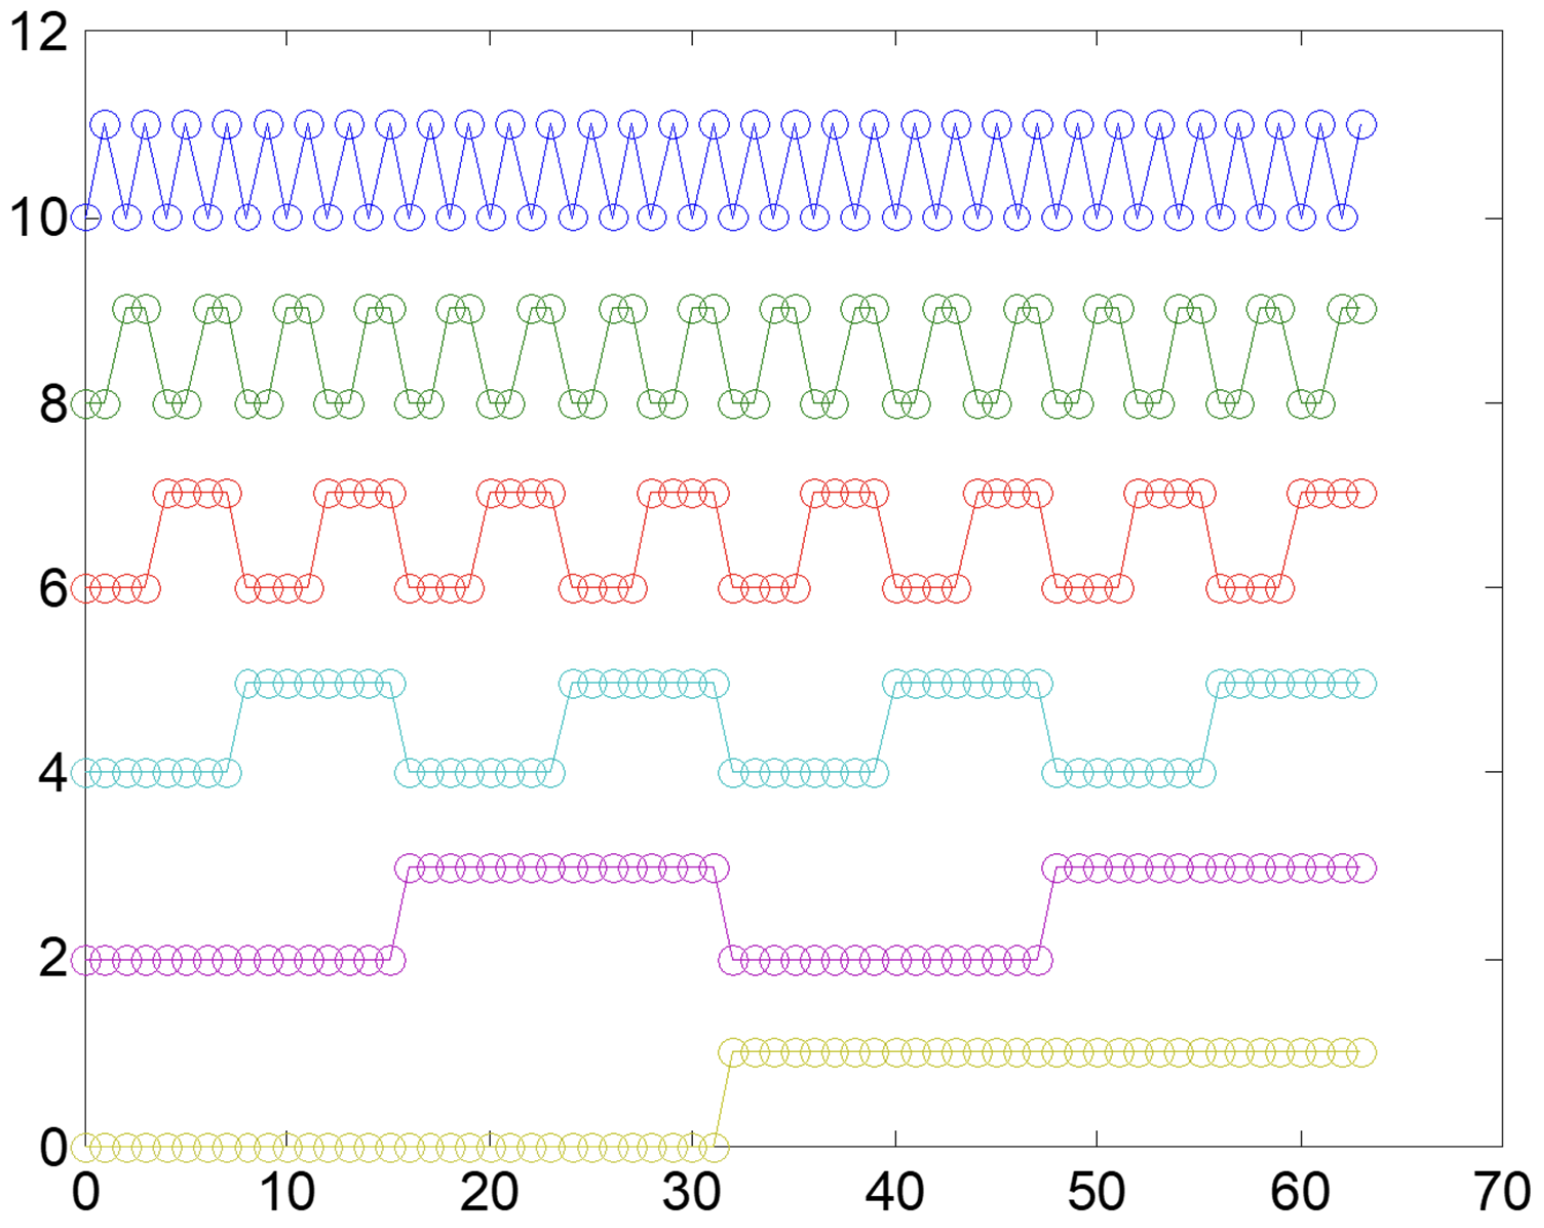
\includegraphics[width=1\textwidth]{rappresentazione-codice-binario.png}
        \caption{Rappresentazione codice binario}
        \label{fig:rapp_cod_bin}
    \end{subfigure}
    \begin{subfigure}{0.5\textwidth}
        \centering
        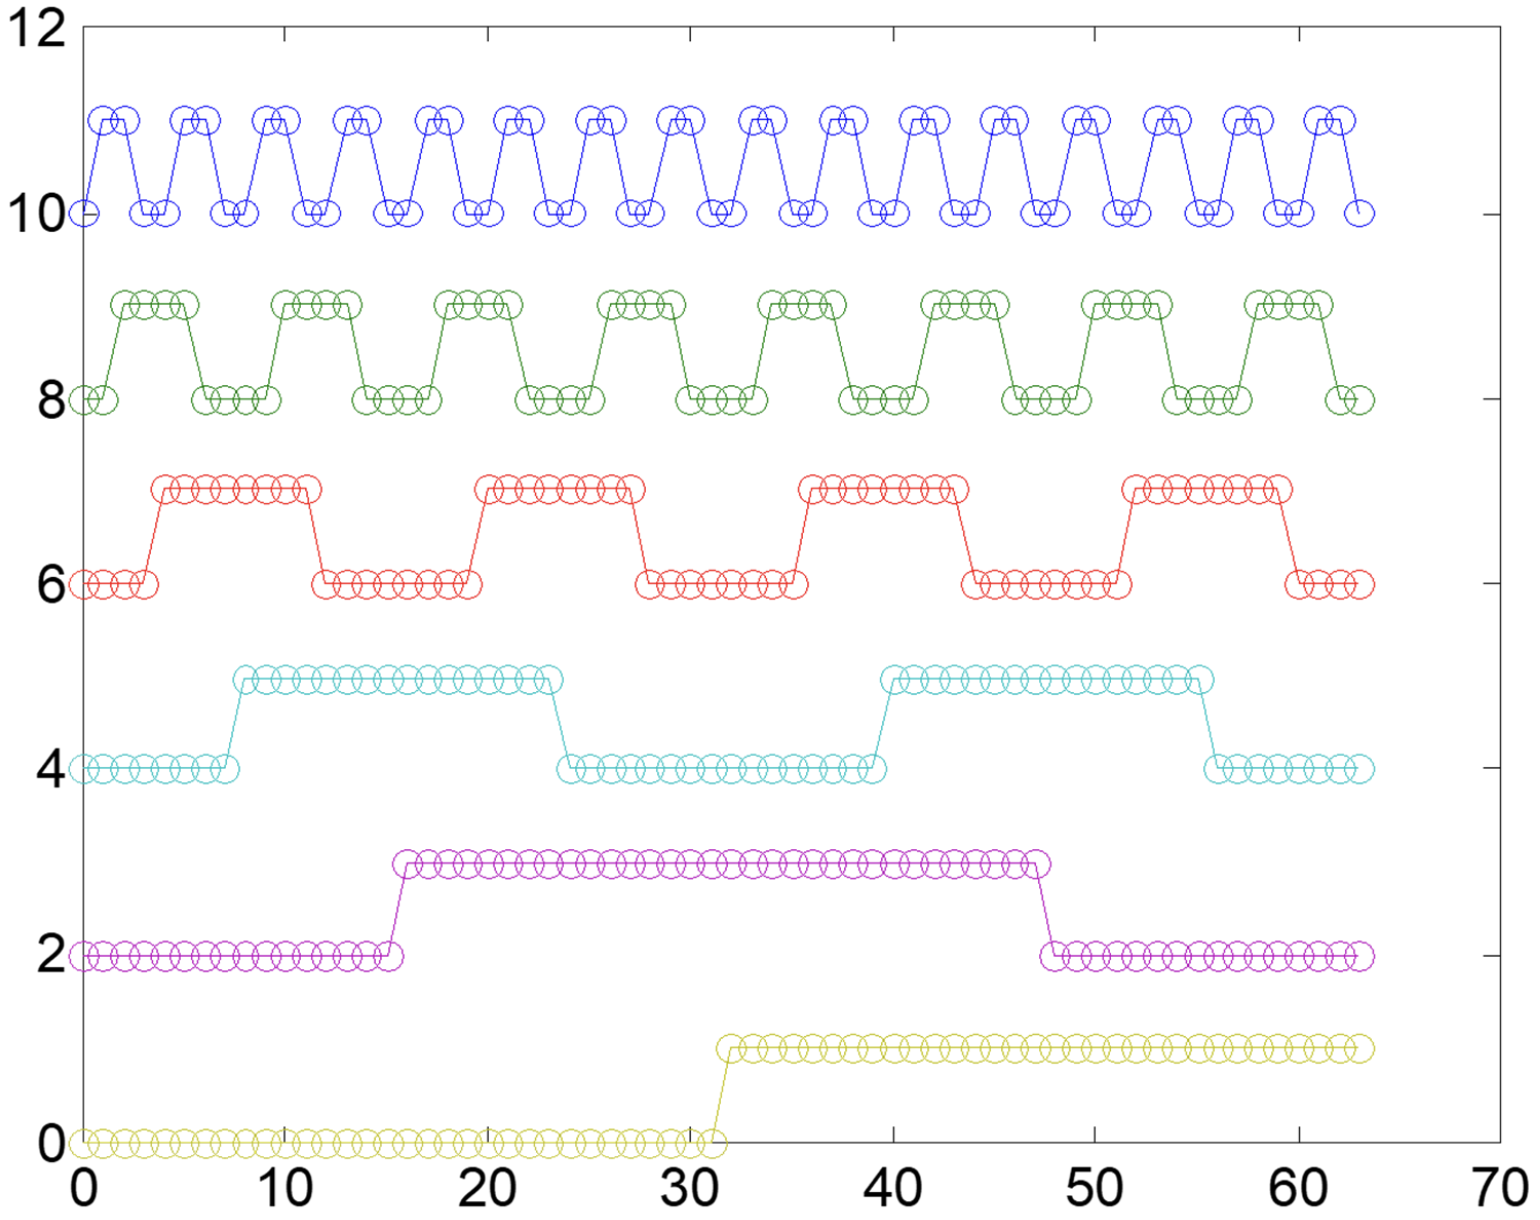
\includegraphics[width=1\textwidth]{rappresentazione-codice-gray.png}
        \caption{Rappresentazione codice di Gray}
        \label{fig:rapp_cod_gray}
    \end{subfigure}
\end{figure}

\vspace{1em}
\noindent
Dai grafici di cui sopra è facile capire che grazie al codice di Gray, ad ogni step, vi è sempre uno e un solo bit che commuta, mentre nel caso del codice binario, possono anche commutare tutti simultaneamente.\\
Non solo, ma il codice di Gray e il codice binario vengono impiegati come \textbf{divisori di frequenza}.

\vspace{1em}
\subsubsection{Conversione Gray-Binario}
La conversione Gray-Binario è particolarmente semplice. Infatti
\begin{itemize}
    \item per passare da Gray a Binario, procedendo da sinistra verso destra, si copia il primo bit inalterato; dopodiché analizzando ad uno ad uno i bit del codice di Gray
    \begin{itemize}
        \item se si legge $1$, il bit del codice Binario precedente viene commutato;
        \item se si legge $0$ si copia il bit del codice Binario precedente inalterato;
    \end{itemize}
    come mostrato nel seguito:

    \noindent
    \begin{table}[H]
    \rowcolors{1}{white}{white}
    \setlength{\tabcolsep}{4pt}
    \renewcommand{\arraystretch}{1.2}
    \centering
    \begin{tabular}{|l|c|c|c|c|c|c|c|c|c|c|c|}
        \hline
        Gray & 1 & 0 & 1 & 1 & 1 & 1 & 0 & 1 & 0 & 0 & 1\\
        \hline
        op. & $\downarrow$ & = & com. & com. & com. & com. & = & com. & = & = & com.\\
        \hline
        Binario & 1 & 1 & 0 & 1 & 0 & 1 & 1 & 0 & 0 & 0 & 1\\
        \hline
    \end{tabular}
    \end{table}

    \item per passare da Binario a Gray, procedendo da sinistra verso destra, si copia il primo bit inalterato; dopodiché analizzando ad uno ad uno i bit del codice Binario
    \begin{itemize}
        \item se il bit del codice di Binario corrente e quello precedente sono uguali, allora si scrive $0$;
        \item se il bit del codice di Binario corrente e quello precedente sono diversi, allora si scrive $1$;
    \end{itemize}
    come mostrato nel seguito:

    \noindent
    \begin{table}[H]
    \rowcolors{1}{white}{white}
    \setlength{\tabcolsep}{4pt}
    \renewcommand{\arraystretch}{1.2}
    \centering
    \begin{tabular}{|l|c|c|c|c|c|c|c|c|c|c|c|}
        \hline
        Binario & 1 & 1 & 0 & 1 & 0 & 1 & 1 & 0 & 0 & 0 & 1\\
        \hline
        op. & $\downarrow$ & = & $\neq$ & $\neq$ & $\neq$ & $\neq$ & = & $\neq$ & = & = & $\neq$\\
        \hline
        Gray & 1 & 0 & 1 & 1 & 1 & 1 & 0 & 1 & 0 & 0 & 1\\
        \hline
    \end{tabular}
    \end{table}
\end{itemize}

\newpage
\begin{center}
    18 Ottobre 2022
\end{center}
\section{Algebra Booleana}
L'Algebra Booleana è nata per studiare problemi di logica deduttiva e prevede la presenza di $2$ soli elementi, $0$ e $1$, rappresentabili tramite delle \textbf{variabili logiche}, ossia grandezze che assumono solo i valori $1$ o $0$.\\
In tale contesto, una \textbf{funzione logica} rappresenta la dipendenza di una grandezza logica da altre grandezze logiche. È immediato evincere che le funzioni logiche in $n$ variabili sono finite e pari $2^{2^n}$.\\
In funzione logica è rappresentabile con una “tabella di verità” in essa vi si contemplano tutti i casi possibili

\vspace{1em}
\subsection{Funzioni ad una variabile}
Le funzioni ad $1$ variabile sono $2^{2^1}=4$, ossia le seguenti, descritte tramite le \textbf{tabelle di verità}:

\noindent
\begin{table}[H]
\rowcolors{1}{white}{white}
\setlength{\tabcolsep}{4pt}
\renewcommand{\arraystretch}{1.2}
\centering
\begin{tabular}{cccc}
    {
        \begin{tabular}{|c|c|}
            \hline
            $x$&$y$\\
            \hline
            $0$&$0$\\
            \hline
            $1$&$0$\\
            \hline
        \end{tabular}
    }&
    {
        \begin{tabular}{|c|c|}
            \hline
            $x$&$y$\\
            \hline
            $0$&$0$\\
            \hline
            $1$&$1$\\
            \hline
        \end{tabular}
    }&
    {
        \begin{tabular}{|c|c|}
            \hline
            $x$&$y$\\
            \hline
            $0$&$1$\\
            \hline
            $1$&$1$\\
            \hline
        \end{tabular}
    }&
    {
        \begin{tabular}{|c|c|}
            \hline
            $x$&$y$\\
            \hline
            $0$&$1$\\
            \hline
            $1$&$0$\\
            \hline
        \end{tabular}
    }
\end{tabular}
\end{table}

\vspace{1em}
in cui, tuttavia, tre funzioni sono degeneri, in quanto
\begin{itemize}
    \item una produce l'uscita costante $0$;
    \item una produce l'uscita costante $1$;
    \item una produce come uscita l'ingresso stesso.
\end{itemize}
L'unica funzione che ha senso considerare è quella che produce in uscita l'opposto dell'ingresso:
\[y=\overline{x}\]
che presenta il simbolo circuitale seguente
% Contenitore per immagini
\begin{figure}[H]
\centering
    \begin{tikzpicture}
        \node (A) at (0,0) {$x$};
        \node (Y) at (2.2,0) {$\overline{x}$};
        \node[not gate US, draw, logic gate inputs=n] at (1,0) (TS) {};
        \draw (A) -- (TS.input);
        \draw (TS.output) -- (Y);
    \end{tikzpicture}
\caption{Negazione (o complementazione)}
\label{fig:negazione_o_complementazione}
\end{figure}

\vspace{1em}
\subsection{Funzioni a due variabili}
Le funzioni a due variabili (in cui \(n = 2\)) che si possono costruire sono
\[2^{2^2} = 2^4 = 16\]
Sono funzioni Booleane di-arie del tipo \(z = f(x, y)\) e sono così importanti da meritare una descrizione anche circuitale.\\
Di seguito vengono riportate usando il linguaggio dell'Algebra Booleana:

\begin{table}[H]
    \centering
    \setlength{\tabcolsep}{10pt}
    \renewcommand{\arraystretch}{1.4}
    \begin{tabularx}{\textwidth}{PP|P>{\hsize=0.015\textwidth}PPPPPPP>{\hsize=0.03\textwidth}P>{\hsize=0.03\textwidth}PPPPPPPPPPP>{\hsize=0.03\textwidth}PP}
         $ $ & $ $ & $f_0$ & $f_1$ & $f_2$ & $f_3$ & $f_4$ & $f_5$ & $f_6$ & $f_7$ & $f_8$ & $f_9$ & $f_{10}$ & $f_{11}$ & $f_{12}$ & $f_{13}$ & $f_{14}$ & $f_{15}$\\
         \hline
         $ $ & $ $ & $ $ & $\hspace{-0.75em} \text{AND}$ & $ $ & $ $ & $ $ & $ $ & $\hspace{-0.95em} \text{XOR}$ & $\hspace{-0.45em}  \text{OR}$ & $\hspace{-0.5em} \text{NOR}$ & $\hspace{-1em} \text{XNOR} \hspace{1em}$ & $ $ & $ $ & $ $ & $ $ & \multicolumn{2}{P}{$\hspace{-3.5em} \text{NAND}$}\\
         $A$ & $B$ & $\textbf{0}$ & $\cdot$ & $ $ & $ $ & $ $ & $ $ & $\oplus$ & $+$ & $\downarrow$ & $\odot$ & $ $ & $ $ & $ $ & $ $ & $\hspace{0.4em} \vert$ & $\textbf{1}$\\
         \hline
         $F$ & $F$ & $F$ & $F$ & $F$ & $F$ & $F$ & $F$ & $F$ & $F$ & $V$ & $V$ & $V$ & $V$ & $V$ & $V$ & $V$ & $V$\\
         $F$ & $V$ & $F$ & $F$ & $F$ & $F$ & $V$ & $V$ & $V$ & $V$ & $F$ & $F$ & $F$ & $F$ & $V$ & $V$ & $V$ & $V$\\
         $V$ & $F$ & $F$ & $F$ & $V$ & $V$ & $F$ & $F$ & $V$ & $V$ & $F$ & $F$ & $V$ & $V$ & $F$ & $F$ & $V$ & $V$\\
         $V$ & $V$ & $F$ & $V$ & $F$ & $V$ & $F$ & $V$ & $F$ & $V$ & $F$ & $V$ & $F$ & $V$ & $F$ & $V$ & $F$ & $V$\\
    \end{tabularx}
    \caption{Tutte le possibili \(2^{2^2} = 16\) funzioni Booleane a due variabili}
    \label{tab:16_funzioni_due_variabili}
\end{table}

\noindent
Tra tutte queste funzioni è noto che alcune sono particolarmente significative, precisamente le sei evidenziate in Tabella \ref{tab:16_funzioni_booleane_con_connettivi_principali}, che sono rispettivamente AND, OR, XOR, NAND, NOR e XNOR; nella tabella seguente esse sono espresse, assieme alle rimanenti, mediante i simboli \(\cdot, +, \oplus, \vert, \downarrow\) e \(\odot\) che si usano tradizionalmente nell'ambito dell'Algebra Booleana; si noti che \(+, \cdot\) e \(\odot\) stanno rispettivamente per \(\cup, \cap\) e \(\equiv\), comunemente utilizzati parlando di connettivi.

\begin{table}[H]
    \centering
    \setlength{\tabcolsep}{10pt}
    \renewcommand{\arraystretch}{1.4}
    \begin{tabularx}{\textwidth}{|l|P||l|P|}
    \hline
        \(f_0 = \textbf{0} \hspace{5em}\) & $ $ & \(f_8 = x \downarrow y \hspace{5em}\) & NOR\\
        \(f_1 = x \cdot y \hspace{5em}\) & AND & \(f_9 = x \odot y \hspace{5em}\) & XNOR\\
        \(f_2 = x \cdot \overline{y} \hspace{5em}\) & $ $ & \(f_{10} = \overline{y} \hspace{5em}\) & $ $\\
        \(f_3 = x \hspace{5em}\) & $ $ & \(f_{11} = x + \overline{y} \hspace{5em}\) & $ $\\
        \(f_4 = \overline{x} \cdot y \hspace{5em}\) & $ $ & \(f_{12} = \overline{x} \hspace{5em}\) & $ $\\
        \(f_5 = y \hspace{5em}\) & $ $ & \(f_{13} = \overline{x} + y \hspace{5em}\) & $ $\\
        \(f_6 = x \oplus y \hspace{5em}\) & XOR & \(f_{14} = x | y \hspace{5em}\) & NAND\\
        \(f_7 = x + y \hspace{5em}\) & OR & \(f_{15} = \textbf{1}\) & $ $\\
        \hline
    \end{tabularx}
    \caption{Le \(16\) funzione Booleane espresse mediante \(\cdot, +, \oplus, \odot, \downarrow, \vert\) e complementazione}
    \label{tab:16_funzioni_booleane_con_connettivi_principali}
\end{table}

\noindent
Come anticipato, data l'estrema importanza, in ambito circuitale, delle funzioni AND, OR, XOR, NAND, NOR e XNOR, dette anche operatori Booleani, vengono analizzate singolarmente di seguito:

\begin{itemize}
    \item \textbf{Porta AND}\\
    È detta anche \textbf{prodotto logico}. La porta AND restituisce \(0\) in uscita se anche uno solo dei due valori d’ingresso è pari a \(0\); restituisce \(1\) solo quando entrambi gli ingressi sono a \(1\). Il simbolo circuitale è:

    \vspace{1em}
    \rowcolors{1}{white}{white}
    \noindent
    \begin{tabularx}{\textwidth}{PPP}
    {
        \begin{tabular}{c|c}
             \(x\) & \(y\)\\
             \hline
             $0$ & $0$\\
             $0$ & $1$\\
             $1$ & $0$\\
             $1$ & $1$
        \end{tabular}
    }
    &
    {
        \begin{tikzpicture}
            \node [and gate US, draw, logic gate inputs =nn] (and){};
            \draw (and.input 1) -- node[at end, above left]{$x$} ++(left:4mm);
            \draw (and.input 2) -- node[at end, below left]{$y$} ++(left:4mm);
            \draw (and.output) -- node[at end,right]{$x \cdot y$} ++(right:4mm);
        \end{tikzpicture}
    }
    &
    {
        \begin{tabular}{c}
             \(x \cdot y\)\\
             \hline
             $0$\\
             $0$\\
             $0$\\
             $1$
        \end{tabular}
    }\\
    \end{tabularx}
    \vspace{1em}
    \noindent
    Le proprietà fondamentali di tale operatore vengono esposte di seguito:
    \begin{align*}
        &x \cdot 0 = 0 && &x \cdot 1 =x\\
        &x \cdot x = x && &x \cdot \overline{x}=0\\
    \end{align*}
    Inoltre gode della proprietà commutativa
    \[x_1 \cdot x_2 = x_2 \cdot x_1\]
    e della proprietà associativa
    \[(x_1 \cdot x_2) \cdot x_3 = x_1 \cdot (x_2 \cdot x_3)\]

    \vspace{1em}
    \noindent
    \item \textbf{Porta OR}\\
    È detta anche \textbf{somma logica}. La porta OR restituisce \(1\) in uscita se almeno uno dei due valori d’ingresso è pari a \(1\); restituisce \(0\) solo quando entrambi gli ingressi sono a \(0\). Il simbolo circuitale è:

    \vspace{1em}
    \rowcolors{1}{white}{white}
    \noindent
    \begin{tabularx}{\textwidth}{PPP}
    {
        \begin{tabular}{c|c}
             \(x\) & \(y\)\\
             \hline
             $0$ & $0$\\
             $0$ & $1$\\
             $1$ & $0$\\
             $1$ & $1$
        \end{tabular}
    }
    &
    {
    \begin{tikzpicture}
        \node [or gate US, draw, logic gate inputs =nn] (or){};
        \draw (or.input 1) -- node[at end, above left]{$x$} ++(left:4mm);
        \draw (or.input 2) -- node[at end, below left]{$y$} ++(left:4mm);
        \draw (or.output) -- node[at end,right]{$x + y$} ++(right:4mm);
    \end{tikzpicture}
    }
    &
    {
        \begin{tabular}{c}
             \(x + y\)\\
             \hline
             $0$\\
             $1$\\
             $1$\\
             $1$
        \end{tabular}
    }\\
    \end{tabularx}
    \vspace{1em}
    \noindent
    Le proprietà fondamentali di tale operatore vengono esposte di seguito:
    \begin{align*}
        &x + 0 = x && &x + 1 =1\\
        &x + x = x && &x + \overline{x}=1\\
    \end{align*}
    Inoltre gode della proprietà commutativa
    \[x_1 + x_2 = x_2 + x_1\]
    e della proprietà associativa
    \[(x_1 + x_2) + x_3 = x_1 + (x_2 + x_3)\]

    \vspace{1em}
    \noindent
    \item \textbf{Porta XOR}\\
    È l’OR esclusivo. La porta XOR restituisce \(1\) in uscita se o uno o l’altro dei due valori d’ingresso è pari a \(1\), ma non entrambi; restituisce \(0\) quando entrambi gli ingressi sono a \(0\) o a \(1\). Il simbolo circuitale è

    \vspace{1em}
    \rowcolors{1}{white}{white}
    \noindent
    \begin{tabularx}{\textwidth}{PPP}
    {
        \begin{tabular}{c|c}
             \(x\) & \(y\)\\
             \hline
             $0$ & $0$\\
             $0$ & $1$\\
             $1$ & $0$\\
             $1$ & $1$
        \end{tabular}
    }
    &
    {
      \begin{tikzpicture}
          \node [xor gate US, draw, logic gate inputs =nn] (xor){};
          \draw (xor.input 1) -- node[at end, above left]{$x$} ++(left:4mm);
          \draw (xor.input 2) -- node[at end, below left]{$y$} ++(left:4mm);
          \draw (xor.output) -- node[at end,right]{$x \oplus y$} ++(right:4mm);
      \end{tikzpicture}
    }
    &
    {
        \begin{tabular}{c}
             \(x \oplus y\)\\
             \hline
             $0$\\
             $1$\\
             $1$\\
             $0$
        \end{tabular}
    }\\
    \end{tabularx}
    \vspace{1em}
    \noindent
    Le proprietà fondamentali di tale operatore vengono esposte di seguito:
    \begin{align*}
        &x \oplus 0 = x && &x \oplus 1 =\overline{x}\\
        &x \oplus x = 0 && &x \oplus \overline{x}=1\\
    \end{align*}
    ciò suggerisce che lo XOR è un \textbf{invertitore pilotato}. Inoltre gode della proprietà commutativa
    \[x_1 \oplus x_2 = x_2 \oplus x_1\]
    e della proprietà associativa
    \[(x_1 \oplus x_2) \oplus x_3 = x_1 \oplus (x_2 \oplus x_3)\]
\end{itemize}

\vspace{1em}
\noindent
\textbf{Osservazione}: Si osservi che per somma (OR) e prodotto (AND) logico vale la \textbf{proprietà distributiva}, ovvero
\begin{align*}
    (x_1 \cdot x_2) + (x_1 \cdot x_3) = x_1 \cdot (x_2 + x_3)\\
    (x_1 + x_2) \cdot (x_1 + x_3) = x_1 + (x_2 \cdot x_3)\\
\end{align*}
cosa che è facilmente dimostrabile o tramite le tabelle di verità, oppure ragionando sul significato dell'operazione.

\vspace{1em}
\noindent
\begin{itemize}
\item \textbf{Porta NAND}\\
    È la negazione della porta AND, rappresentata dal seguente simbolo circuitale:

    \vspace{1em}
    \rowcolors{1}{white}{white}
    \noindent
    \begin{tabularx}{\textwidth}{PPP}
    {
        \begin{tabular}{c|c}
             \(x\) & \(y\)\\
             \hline
             $0$ & $0$\\
             $0$ & $1$\\
             $1$ & $0$\\
             $1$ & $1$
        \end{tabular}
    }
    &
    {
      \begin{tikzpicture}
          \node [nand gate US, draw, logic gate inputs =nn] (nand){};
          \draw (nand.input 1) -- node[at end, above left]{$x$} ++(left:4mm);
          \draw (nand.input 2) -- node[at end, below left]{$y$} ++(left:4mm);
          \draw (nand.output) -- node[at end,right]{$x \vert y$} ++(right:4mm);
      \end{tikzpicture}
    }
    &
    {
        \begin{tabular}{c}
             \(x \vert y\)\\
             \hline
             $1$\\
             $1$\\
             $1$\\
             $0$
        \end{tabular}
    }\\
    \end{tabularx}
    \vspace{1em}
    \noindent
    Le proprietà fondamentali di tale operatore vengono esposte di seguito:
    \begin{align*}
        &x \vert 0 = 1 && &x \vert 1 =\overline{x}\\
        &x \vert x = \overline{x} && &x \vert \overline{x}=1\\
    \end{align*}
    Inoltre gode della proprietà commutativa
    \[x_1 \vert x_2 = x_2 \vert x_1\]
    ma \textbf{non gode} della proprietà associativa, in quanto non è vero che
    \[(x_1 \vert x_2) \vert x_3 \neq x_1 \vert (x_2 \vert x_3)\]

    \vspace{1em}
    \noindent
    Com'è noto, la porta NAND è un \textbf{operatore universale}, nel senso che da sola consente di costruire una qualunque tra le \(16\) possibili funzioni. Per declinare le relazioni succitate nei termini del linguaggio dell'Algebra Booleana è sufficiente usare gli assiomi e i teoremi visti in precedenza:
    \begin{align*}
        \overline{x} = \overline{x \cdot x} = x | x\\
        x + y = \overline{\overline{x} \cdot \overline{y}} = \overline{x} | \overline{y}\\
        x \cdot y = \overline{\overline{x \cdot y}} = \overline{x | y}
     \end{align*}
     Da cui derivano le seguenti rappresentazioni circuitali:

     % Contenitore per immagini
     \rowcolors{1}{white}{white}
     \noindent
     \begin{table}[H]
         \centering
         \noindent
         \begin{tabularx}{\textwidth}{PPP}
              {
                \begin{tikzpicture}
                    \coordinate (start) at (-1.5,-0.8);
                    \node [nand gate US, draw, logic gate inputs=nn] (nand){};

                    \draw (-0.6,0) -- node[at end, left]{$x$} (-0.8,0);
                    \draw (nand.input 2) ++(-0.3,0.08) node [branch]{} |- (nand.input 1);
                    \draw (nand.input 1) ++(-0.3,-0.08) node []{} |- (nand.input 2);
                    \draw (nand.output) -- ([xshift=0.3cm] nand.output) node [right] {{$\overline{x}$}};
                \end{tikzpicture}
              }
              &
              {
                \hspace{-2em}
                \begin{tikzpicture}
                  \node [nand gate US, draw, logic gate inputs=nn] (nand1){};
                  \node [nand gate US, draw, below=of nand1, yshift=5.5mm, logic gate inputs=nn] (nand2){};
                  \node [nand gate US, draw, right=of nand1, xshift=-3mm, yshift=-5mm, logic gate inputs=nn] (nand3){};

                  \draw (-0.6,0) -- node[at end, left]{$x$} (-0.8,0);
                  \draw (nand1.input 2) ++(-0.3,0.08) node [branch]{} |- (nand1.input 1);
                  \draw (nand1.input 1) ++(-0.3,-0.08) node []{} |- (nand1.input 2);

                  \draw (-0.6,-0.97) -- node[at end, left]{$y$} (-0.8,-0.97);
                  \draw (nand2.input 2) ++(-0.3,0.08) node [branch]{} |- (nand2.input 1);
                  \draw (nand2.input 1) ++(-0.3,-0.08) node []{} |- (nand2.input 2);

                  \draw (nand1.output) -- ([xshift=0.3cm] nand1.output) |- (nand3.input 1);
                  \draw (nand2.output) -- ([xshift=0.3cm] nand2.output) |- (nand3.input 2);
                  \draw (nand3.output) -- ([xshift=0.3cm] nand3.output) node [right] {{$x + y$}};
                \end{tikzpicture}
              }
              &
              {
                \begin{tikzpicture}
                  \coordinate (start) at (-0.7,0);
                  \node [nand gate US, draw, logic gate inputs=nn] (nand1){};
                  \node [nand gate US, draw, right=of nand1, logic gate inputs=nn] (nand2){};

                  \draw (nand1.input 1) -- node[at end, above left]{$x$} (nand1.input 1 -| start);
                  \draw (nand1.input 2) -- node[at end, below left]{$y$} (nand1.input 2 -| start);

                  \draw (nand1.output) -- ([xshift=0.3cm] nand1.output) node [branch]{} |- (nand2.input 1);
                  \draw (nand1.output) -- ([xshift=0.3cm] nand1.output) node []{} |- (nand2.input 2);

                  \draw (nand2.output) -- ([xshift=0.3cm] nand2.output) node [right] {{$x \cdot y$}};
                \end{tikzpicture}
              }
         \end{tabularx}\\
         \caption{Funzioni NOT, OR e AND realizzazate mediante la porta universale NAND}
         \label{tab:NOT_OR_AND_tramite_NAND}
     \end{table}

    \item \textbf{Porta NOR}\\
    È la negazione della porta OR, rappresentata dal seguente simbolo circuitale:

    \vspace{1em}
    \rowcolors{1}{white}{white}
    \noindent
    \begin{tabularx}{\textwidth}{PPP}
    {
        \begin{tabular}{c|c}
             \(x\) & \(y\)\\
             \hline
             $0$ & $0$\\
             $0$ & $1$\\
             $1$ & $0$\\
             $1$ & $1$
        \end{tabular}
    }
    &
    {
      \begin{tikzpicture}
          \node [nor gate US, draw, logic gate inputs =nn] (nor){};
          \draw (nor.input 1) -- node[at end, above left]{$x$} ++(left:4mm);
          \draw (nor.input 2) -- node[at end, below left]{$y$} ++(left:4mm);
          \draw (nor.output) -- node[at end,right]{$x \downarrow y$} ++(right:4mm);
      \end{tikzpicture}
    }
    &
    {
        \begin{tabular}{c}
             \(x \downarrow y\)\\
             \hline
             $1$\\
             $0$\\
             $0$\\
             $0$
        \end{tabular}
    }\\
    \end{tabularx}
    \vspace{1em}
    \noindent
    Le proprietà fondamentali di tale operatore vengono esposte di seguito:
    \begin{align*}
        &x \downarrow 0 = \overline{x} && &x \downarrow 1 =0\\
        &x \downarrow x = \overline{x} && &x \downarrow \overline{x}=0\\
    \end{align*}
    Inoltre gode della proprietà commutativa
    \[x_1 \downarrow x_2 = x_2 \downarrow x_1\]
    ma \textbf{non gode} della proprietà associativa, in quanto non è vero che
    \[(x_1 \downarrow x_2) \downarrow x_3 \neq x_1 \downarrow (x_2 \downarrow x_3)\]

    \vspace{1em}
    \noindent
    Com'è noto, anche la porta NOR è un \textbf{operatore universale}, nel senso che da sola consente di costruire una qualunque tra le \(16\) possibili funzioni. Per declinare le relazioni succitate nei termini del linguaggio dell'Algebra Booleana è sufficiente usare gli assiomi e i teoremi visti in precedenza:
    \begin{align*}
        \overline{x} = \overline{x + x} = x \downarrow x\\
        x + y = \overline{\overline{x + y}} = \overline{x \downarrow y}\\
        x \cdot y = \overline{\overline{x} + \overline{y}} = \overline{x} \downarrow \overline{y}
     \end{align*}
     Da cui derivano le seguenti rappresentazioni circuitali:

     % Contenitore per immagini
     \rowcolors{1}{white}{white}
     \noindent
     \begin{table}[H]
         \centering
         \noindent
         \begin{tabularx}{\textwidth}{PPP}
              {
                \begin{tikzpicture}
                    \coordinate (start) at (-1.5,-0.8);
                    \node [nor gate US, draw, logic gate inputs=nn] (nor){};

                    \draw (-0.6,0) -- node[at end, left]{$x$} (-0.8,0);
                    \draw (nor.input 2) ++(-0.3,0.08) node [branch]{} |- (nor.input 1);
                    \draw (nor.input 1) ++(-0.3,-0.08) node []{} |- (nor.input 2);
                    \draw (nor.output) -- ([xshift=0.3cm] nor.output) node [right] {{$\overline{x}$}};
                \end{tikzpicture}
              }
              &
              {
                \hspace{-3em}
                \begin{tikzpicture}
                  \coordinate (start) at (-0.7,0);
                  \node [nor gate US, draw, logic gate inputs=nn] (nor1){};
                  \node [nor gate US, draw, right=of nor1, logic gate inputs=nn] (nor2){};

                  \draw (nor1.input 1) -- node[at end, above left]{$x$} (nor1.input 1 -| start);
                  \draw (nor1.input 2) -- node[at end, below left]{$y$} (nor1.input 2 -| start);

                  \draw (nor1.output) -- ([xshift=0.3cm] nor1.output) node [branch]{} |- (nor2.input 1);
                  \draw (nor1.output) -- ([xshift=0.3cm] nor1.output) node []{} |- (nor2.input 2);

                  \draw (nor2.output) -- ([xshift=0.3cm] nor2.output) node [right] {{$x + y$}};
                \end{tikzpicture}
              }
              &
              {
                \begin{tikzpicture}
                  \node [nor gate US, draw, logic gate inputs=nn] (nor1){};
                  \node [nor gate US, draw, below=of nand1, yshift=5.5mm, logic gate inputs=nn] (nor2){};
                  \node [nor gate US, draw, right=of nand1, xshift=-3mm, yshift=-5mm, logic gate inputs=nn] (nor3){};

                  \draw (-0.6,0) -- node[at end, left]{$x$} (-0.8,0);
                  \draw (nor1.input 2) ++(-0.3,0.08) node [branch]{} |- (nor1.input 1);
                  \draw (nor1.input 1) ++(-0.3,-0.08) node []{} |- (nor1.input 2);

                  \draw (-0.6,-0.97) -- node[at end, left]{$y$} (-0.8,-0.97);
                  \draw (nor2.input 2) ++(-0.3,0.08) node [branch]{} |- (nor2.input 1);
                  \draw (nor2.input 1) ++(-0.3,-0.08) node []{} |- (nor2.input 2);

                  \draw (nor1.output) -- ([xshift=0.3cm] nor1.output) |- (nor3.input 1);
                  \draw (nor2.output) -- ([xshift=0.3cm] nor2.output) |- (nor3.input 2);
                  \draw (nor3.output) -- ([xshift=0.3cm] nor3.output) node [right] {{$x \cdot y$}};
                \end{tikzpicture}
              }
         \end{tabularx}\\
         \caption{Funzioni NOT, OR e AND realizzate mediante la porta universale NOR}
         \label{tab:NOT_OR_AND_tramite_NOR}
     \end{table}
\end{itemize}
E questo è un risultato molto importante dal punto di vista tecnico industriale, dal momento che potrebbero comportare significativi vantaggi dal punto di vista economico-produttivo.

\vspace{1em}
\noindent
\subsection{Tecnologia CMOS}
Le porte NAND e NOR, oltre ad essere degli operatori universali, sono anche particolarmente facili da realizzare con la tecnologia CMOS.\\
La sigma CMOS sta per Complementary MOS, in cui MOS (Metal Oxide Semiconductor) è un particolare tipo di transistor. Un transistor MOS può essere approssimato ad un interruttore, per quanto riguarda il suo funzionamento. La sua struttura viene di seguito esposta:

\begin{figure}[H]
    \centering
    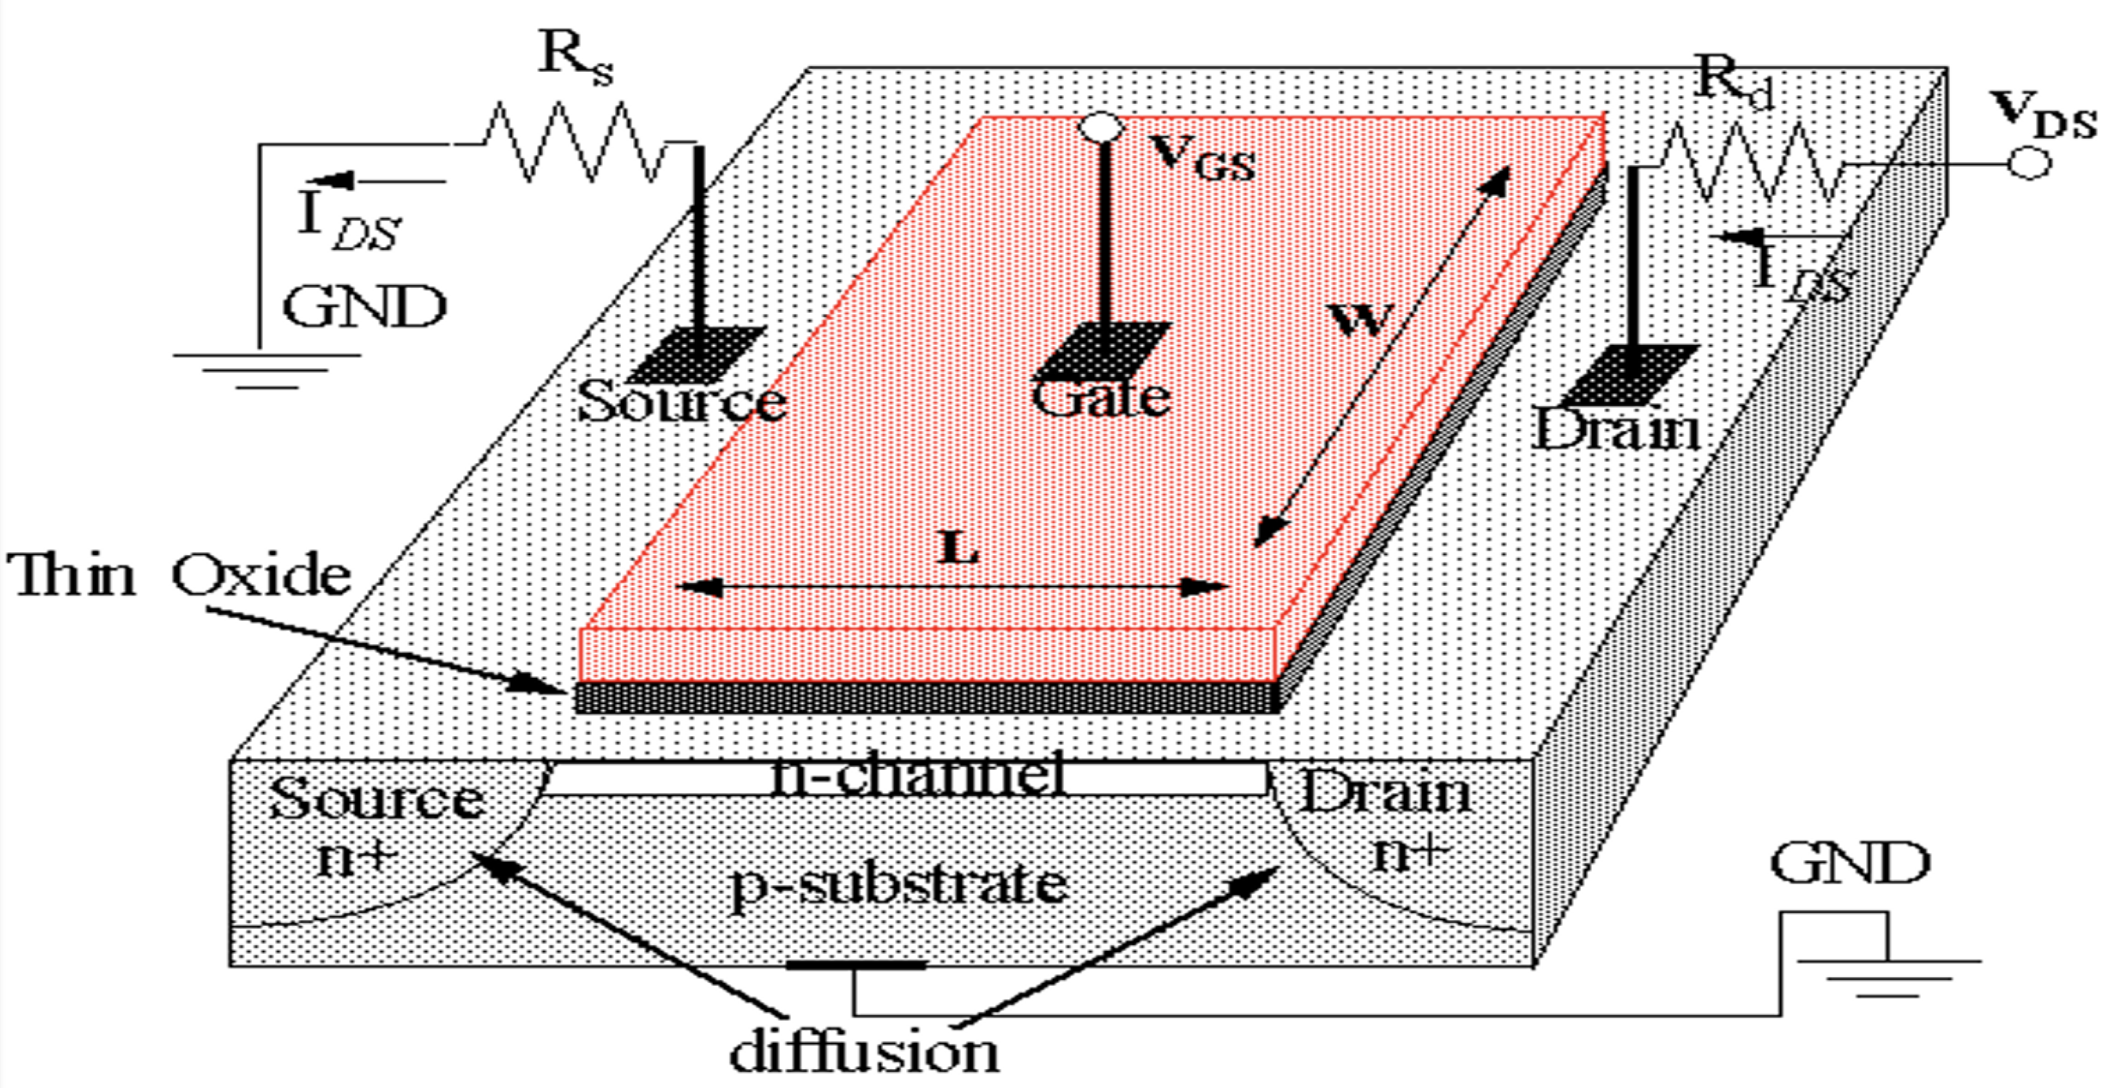
\includegraphics[width=0.5\textwidth]{transistor-cmos-struttura.png}
    \caption{Struttura transistor CMOS}
    \label{fig:transistor_cmos_strut}
\end{figure}

\vspace{1em}
\noindent
in cui appare immediatamente evidente il \textbf{substrato di silicio} (chiamato substrato-p), ricco di cariche positive, realizzato tramite un \textbf{wafer di silicio} neutro che è stato sottoposto a \textbf{drogaggio}, ossia ad un impiantazione di atomi che presentano una ridondanza di cariche positive (ossia una carenza di elettroni nell'orbita più esterna, chiamata \textbf{lacuna}).\\
Dopodiché si scava ai suoi fianchi, realizzando delle zone in cui il silicio è di diversa natura ed è ricco di cariche negative, ottenendo la sorgente e il drenaggio $n^+$.\\
Il fatto che nel substrato-p ci sia una ridondanza di cariche positive non significa che non vi siano cariche negative, ma esse sono solo in minoranza: ciò consente l'agevole transito di cariche negative (ossia di corrente) dall'elettrodo sorgente $n^+$ all'elettrodo drenaggio $n^+$.\\
Pertanto il silicio che si sta considerando presenta
\begin{itemize}
    \item due aree laterali drogate $n$, ricche di cariche negative;
    \item una area centrale drogata $p$, ricca di cariche positive.
\end{itemize}
il fatto che le cariche negative siano concentrate agli estremi e vi sia una grande zona centrale con ridondanza di cariche positive, comporta la difficoltà di conduzione da parte del transistor, il quale si comporta come un \textbf{interruttore aperto}.\\
Ciò che si fa, quindi, è posizionare sopra il silicio una \textbf{piastra conduttiva}, denominata \textbf{gate}, separata dal substrato di silicio attraverso un finissimo strato di ossido, da cui il nome: metallo-ossido-semiconduttore. Quando si applica una tensione al gate, le poche cariche negative presenti nel substrato-p vengono attirate verso la piastra; si crea, quindi, un \textbf{canale conduttivo} tra le due zone drogate $n$ (sorgente $n^+$ e drenaggio $n^+$) e così facendo si chiude il contatto. Ecco che, quindi, si è ottenuto un sistema che funzione come un interruttore controllato in tensione: quando si applica tensione si chiude l'interruttore, quando si toglie tensione, l'interruttore viene chiuso.

\vspace{1em}
\noindent
\textbf{Osservazione}: Si osservi che i transistor MOS appena descritti possono essere realizzati in due modi differenti: a canale $p$ (positivo) o a canale $n$ (negativo), a seconda che le cariche che portano la corrente siano le lacune (la carenza di elettroni) o gli elettroni, rispettivamente. È abbastanza intuibile che il funzionamento dell'uno sia il duale dell'altro: nel MOS a substrato-p e a canale-n bisogna fornire una tensione positiva per attirare le cariche negative e creare il canale; nel MOS a substrato-n e a canale-p bisogna fornire una tensione negativa per attirare le cariche positive e creare il canale.

\vspace{1em}
\noindent
\subsubsection{Invertitore in CMOS}
Un invertitore in tecnologia CMOS viene creato nel modo seguente:

\begin{figure}[H]
    \centering
    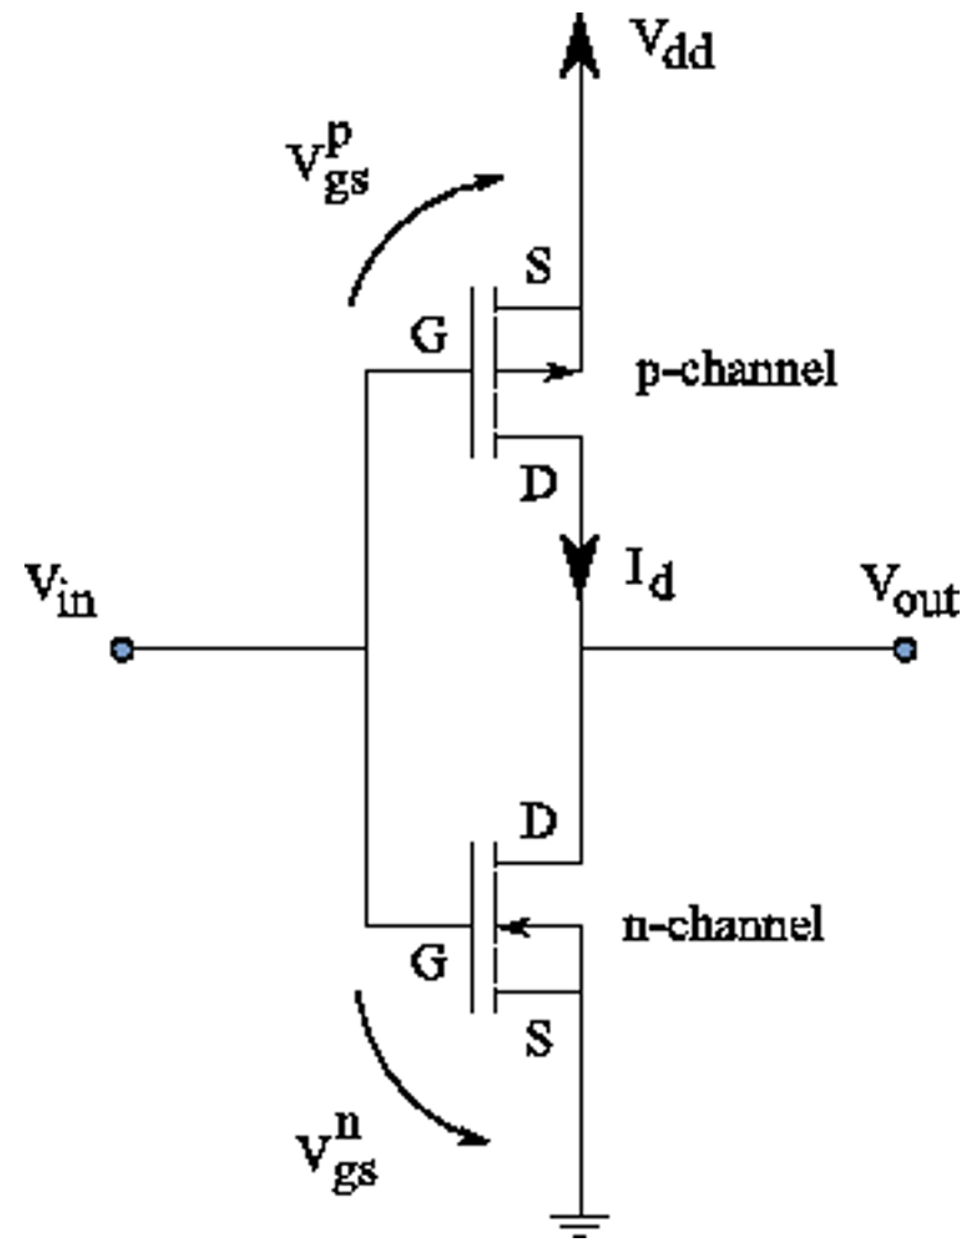
\includegraphics[width=0.35\textwidth]{invertitore-cmos.png}
    \caption{Invertitore in CMOS}
    \label{fig:invertitore_cmos}
\end{figure}

\vspace{1em}
\noindent
in particolare si impilano uno sopra l'altro due transistor CMOS, uno a canale $n$, l'altro a canale $p$: il CMOS a canale $n$ si chiude quando viene fornita una tensione positiva, mentre il CMOS a canale $p$ si chiude quando viene fornita una tensione negativa al gate.\\
In poche parole, tale invertitore funziona come se fossero due interruttori insieme: fornendo in ingresso una tensione $V_{in}$ elevata, il MOS a canale-$p$ rimane aperto, mentre quello che a canale-$n$ si chiude; chiudendosi mette in collegamento l'uscita con la massa alla quale è collegato. Viceversa, fornendo in ingresso una tensione bassa, il transistor a canale-$n$ rimane aperto, mentre il MOS a canale-$p$ si chiude, mettendo in collegamento l'uscita con la tensione di $V_{dd}$ alla quale è collegato.

\vspace{1em}
\noindent
\textbf{Osservazione}: Si osservi che realizzare i transistor MOS finora esposti su silicio non è difficile: è sufficiente prendere in considerare un wafer di silicio e realizzare in esso una zona drogata-$n$ (denominata $n$-well, ossia pozzo $n$), su cui viene creato il transistor a canale-$p$; inoltre si realizza anche una zona drogata $p$ (denominata $p$-well, ossia pozzo $p$), su cui viene creato il transistor a canale $n$.

\vspace{1em}
\noindent
\subsubsection{NOR in CMOS}
Una porta NOR in tecnologia CMOS viene creata nel modo seguente:

\begin{figure}[H]
    \centering
    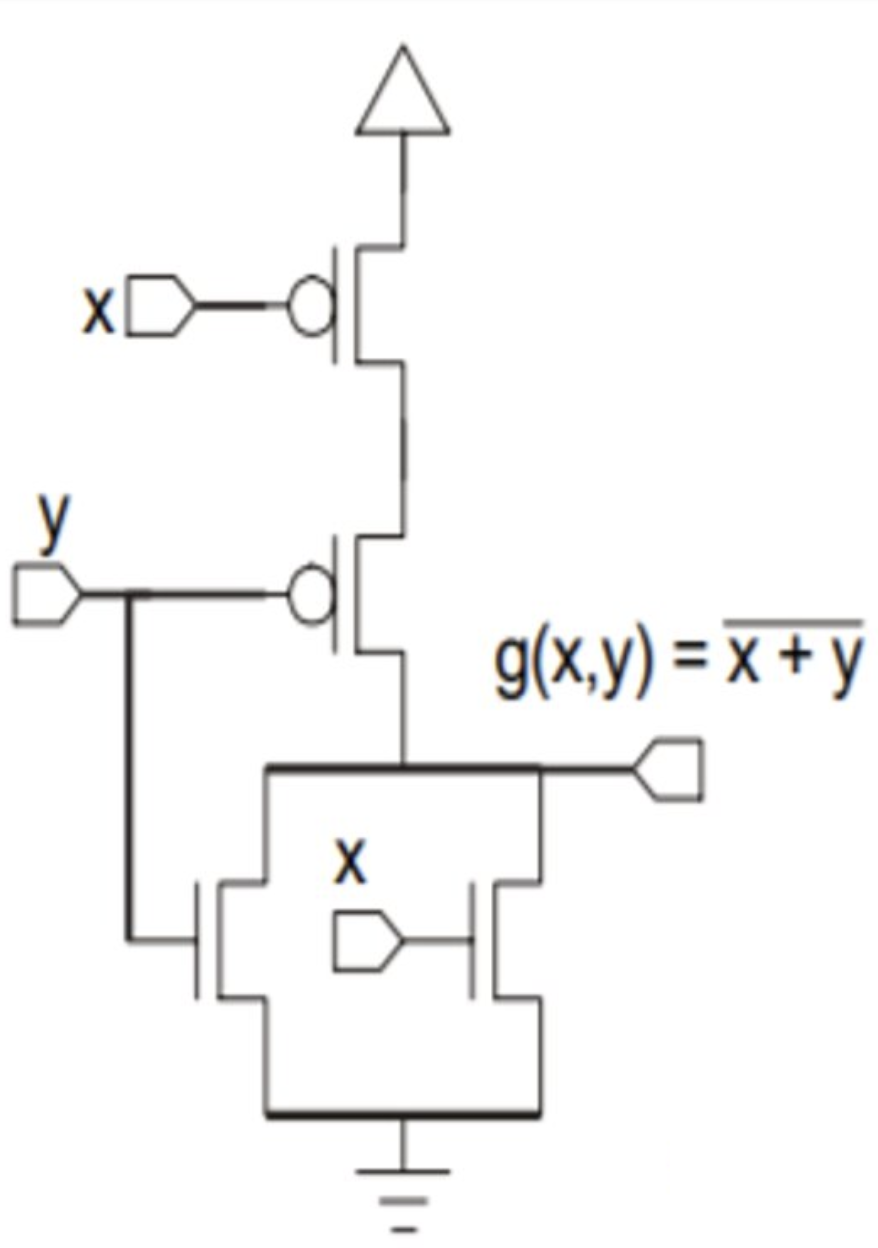
\includegraphics[width=0.25\textwidth]{nor-cmos.png}
    \caption{NOR in CMOS}
    \label{fig:nor_cmos}
\end{figure}

\vspace{1em}
\noindent
In poche parole tale circuito non è altro che un invertitore pilotato da due segnali: quando entrambi i segnali sono a tensione bassa in uscita si ha la tensione $V_{dd}$; invece, se anche uno solo dei segnali in ingresso è a tensione alta, in uscita si ha sempre la tensione di massa. Per realizzare tale porta, vengono semplicemente messi in serie due transistor MOS a canale-$p$ in altro, mentre in parallelo in basso si hanno due transistor a canale-$n$.\\
Siccome una porta NOR produce in uscita il valore $1$ solamente quando in ingresso si hanno due $0$, chiaramente quando si verifica configurazione entrambi i transistor a canale-$p$ saranno in conduzione, ossia chiusi, mentre quelli a canale-$n$ saranno aperti, per cui in uscita si ha il valore di $V_{dd}$. Se, anche uno solo degli ingressi va a $1$, allora almeno uno dei transistor a canale-$p$ sarà aperto, scollegando il circuito dalla tensione di $V_{dd}$; invece, almeno uno dei transistor a canale-$n$ sara in conduzione, collegando inevitabilmente l'uscita a massa.

\vspace{1em}
\noindent
\subsubsection{NAND in CMOS}
Una porta NAND in tecnologia CMOS viene creata nel modo seguente:

\begin{figure}[H]
    \centering
    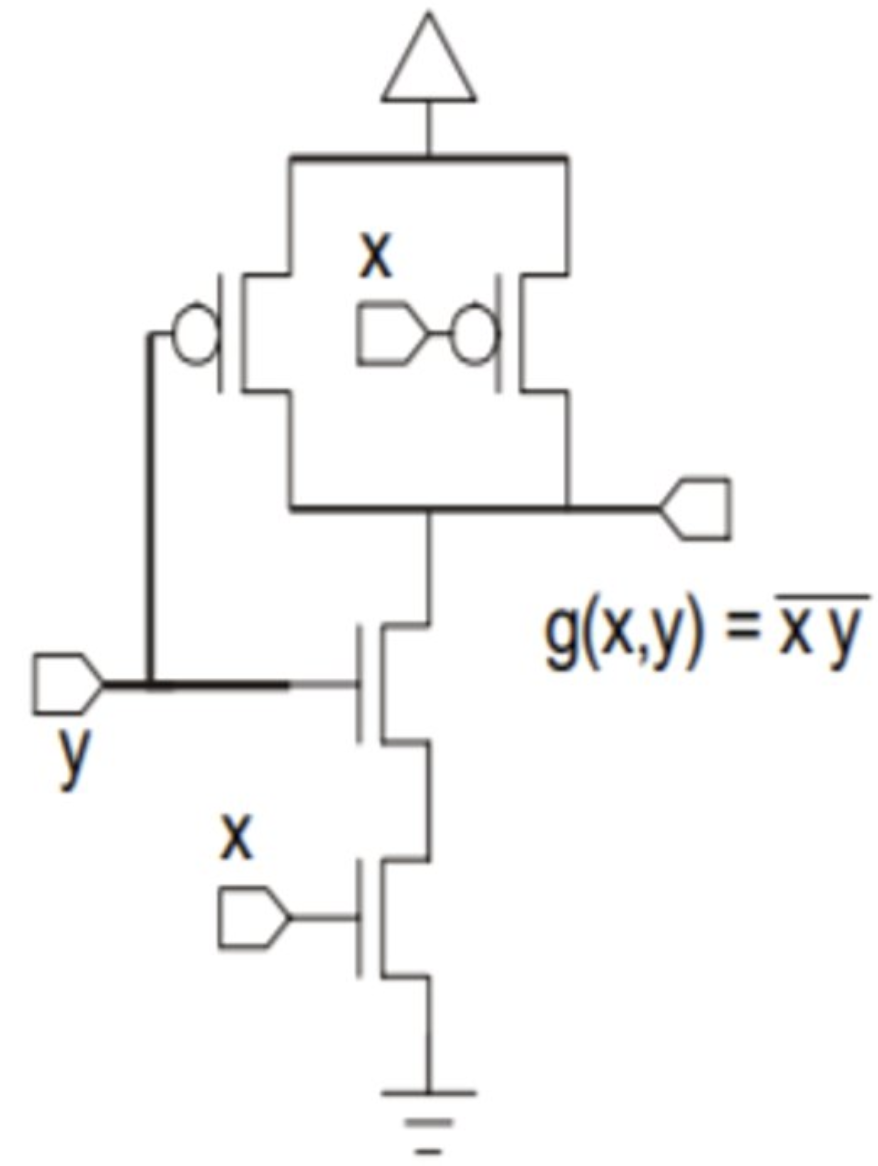
\includegraphics[width=0.25\textwidth]{nand-cmos.png}
    \caption{NAND in CMOS}
    \label{fig:nand_cmos}
\end{figure}

\vspace{1em}
\noindent
Come in precedenza, si sta considerando un circuito approssimabile a un interruttore pilotato da due ingressi; com'è noto, una porta NAND produce in uscita il valore $0$ solamente quando entrambi gli ingressi sono posti a $1$: ciò significa che si necessita di disporre di due transistor a canale-$n$ posti in serie e collegati a massa e di due transistor a canale-$p$ collegati in parallelo e a $V_{dd}$. In questo modo, quando entrambi gli ingressi sono posti a $1$, tutti i transistor a canale-$n$ saranno in conduzione, mentre quelli a canale-$p$ saranno aperti, collegando l'uscita direttamente con la massa. Viceversa, quando almeno uno degli ingressi ha valore basso, almeno uno dei transistor a canale-$p$ è in conduzione e sicuramente almeno uno dei transistor a canale-$n$ è aperto: in questo modo il sistema viene scollegato dalla massa e sempre collegato a $V_{dd}$.

\vspace{1em}
\noindent
\textbf{Osservazione}: Applicando ciclicamente tale logica è possibile realizzare anche una NAND a più ingressi, come mostrata di seguito, sempre sfruttando il colelgamento in serie/parallelo dei transistor a canale-$p$ e a canale-$n$:

\begin{figure}[H]
    \centering
    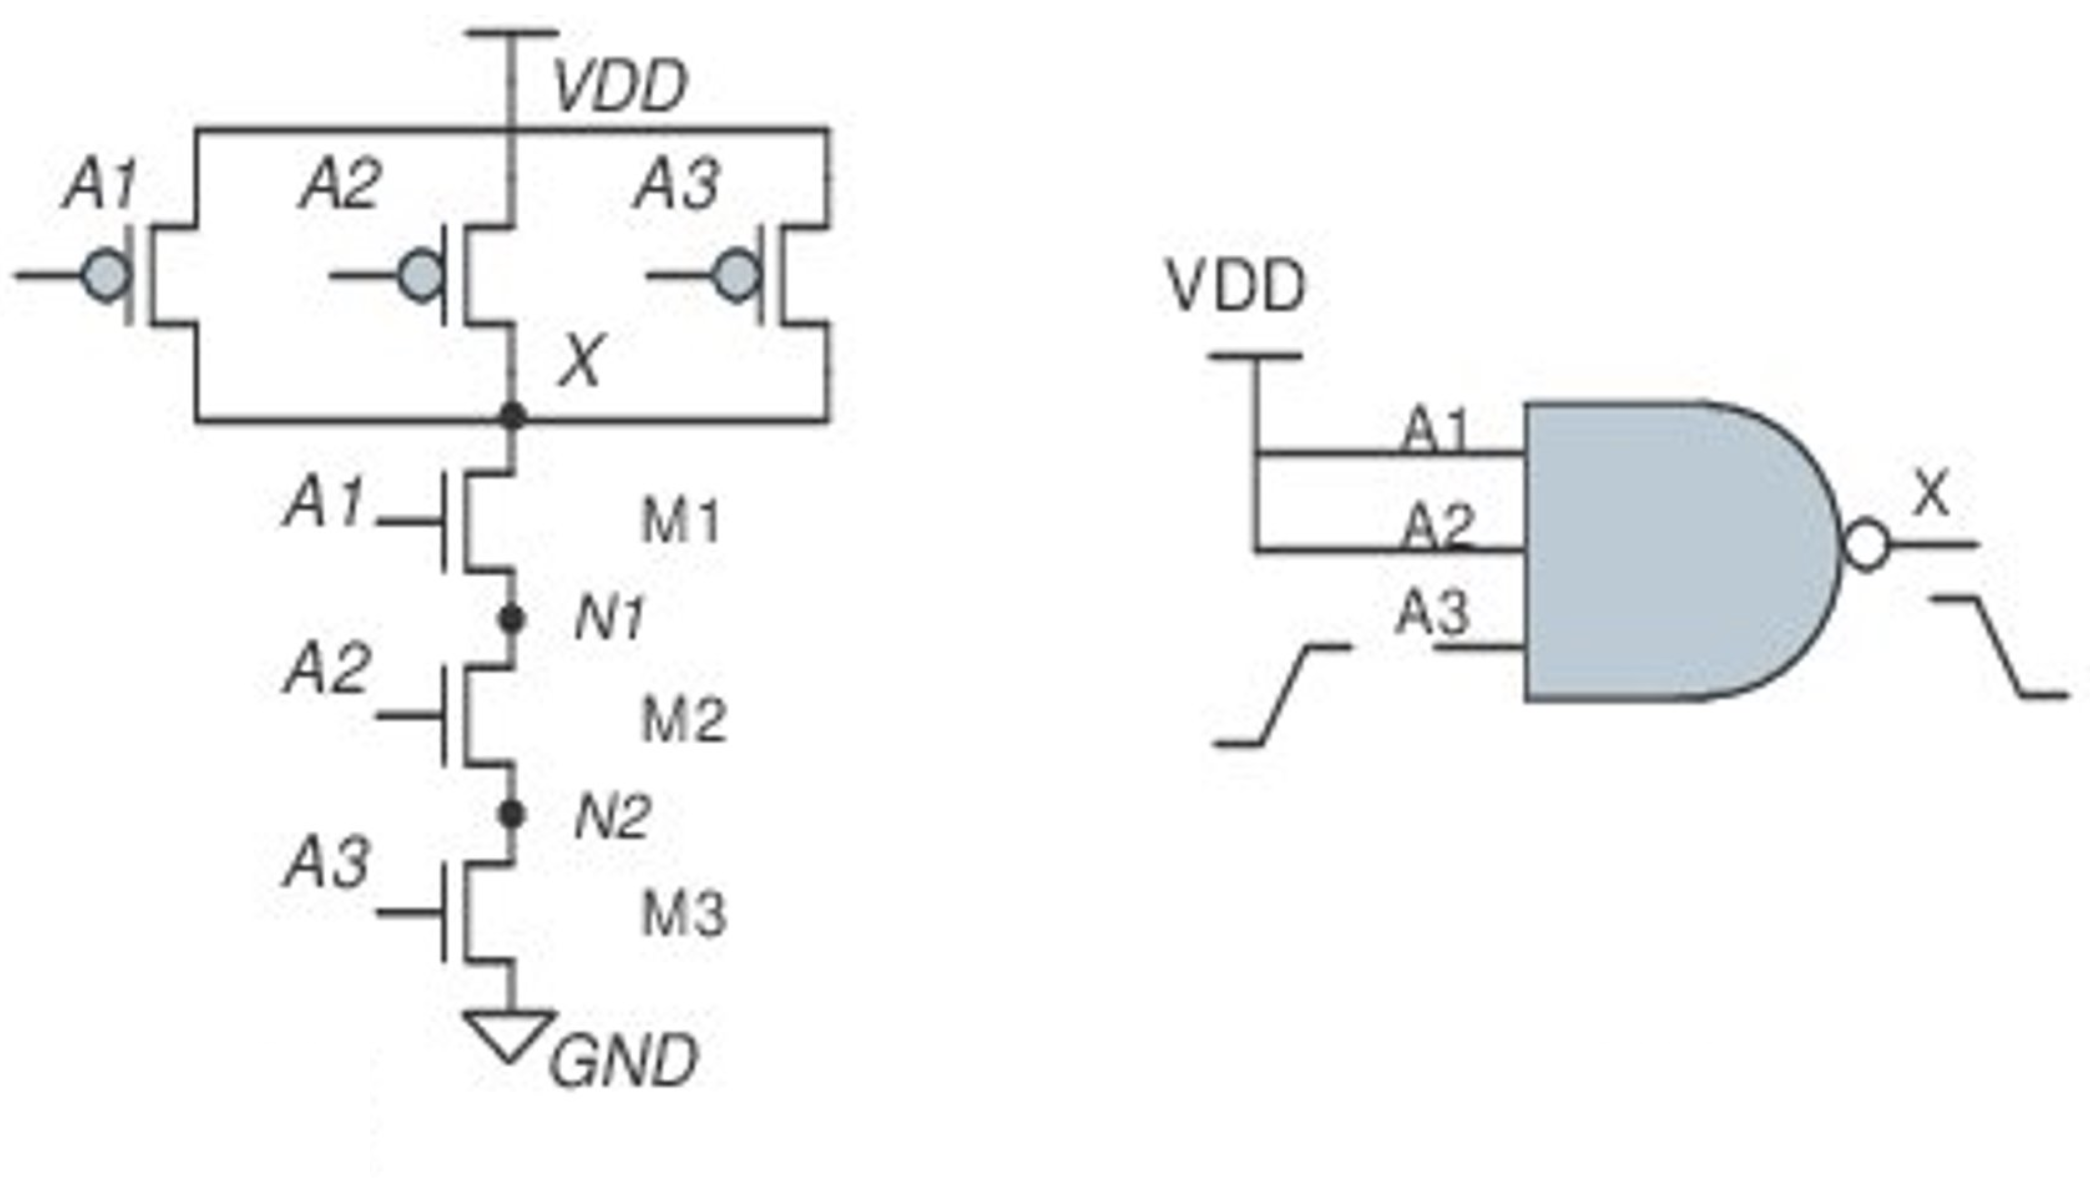
\includegraphics[width=0.5\textwidth]{nand-cmos-piu-ingressi.png}
    \caption{NAND a più ingressi in CMOS}
    \label{fig:nand_pi_ingressi_cmos}
\end{figure}

\vspace{1em}
\noindent
in cui i transistor a canale-$n$ in basso prendono il nome di transistor di \textbf{pull-down}, mentre i transistor a canale-$p$ in alto prendono il nome di transistor di \textbf{pull-up}. Da notare che è molto difficile realizzare porte con numerosi ingressi (ossia con un \textbf{fan-in} elevato) in quanto, com'è noto, nelle serie la tensione si ripartisce tra i diversi transistor e il transistor in testa non possiede sufficiente tensione per attirare le cariche del substrato.

\vspace{1em}
\noindent
\subsubsection{AOI e OAI in CMOS}
Tramite la tecnologia CMOS è possibile realizzare funzioni logiche anche molto complesse, come la funzione $\overline{CB + A}$, che viene creata nel modo seguente:

\begin{figure}[H]
    \centering
    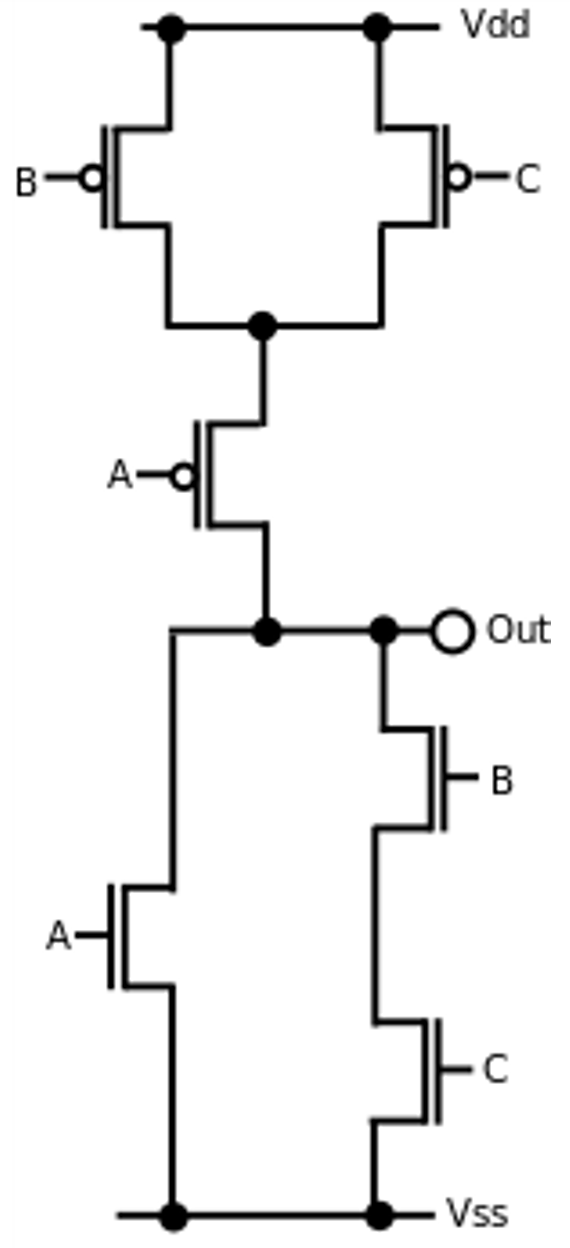
\includegraphics[width=0.2\textwidth]{aoi-oai-cmos.png}
    \caption{AOI e OAI in CMOS}
    \label{fig:aoi_oai_cmos}
\end{figure}

\vspace{1em}
\noindent
in cui, dal momento che è presente una porta NOR, quando tutti gli ingressi della stessa sono a $0$, bisogna produrre in uscite il valore $1$. Questo si fa semplicemente mettendo in serie un transistor a canale-$p$ pilotato dall'ingresso $A$ e un parallelo di due transistor a canale-$p$ pilotati dagli ingressi $B$ e $C$: questo perché, in forza della presenza della porta AND, quando almeno uno degli ingressi è a $0$, si produce in uscita il valore $0$, che posto in serie con l'ingresso $A$ produce il circuito cercato.\\
Per dualità, se in pull-up si ha una serie con un parallelo, in pull-down si dovrà avere un parallelo con una serie.


\vspace{1em}
\noindent
\subsubsection{AOI e OAI in CMOS a 4 ingressi}
Tramite la tecnologia CMOS è possibile realizzare funzioni logiche anche molto complesse, come la funzione $\overline{AB+CD}$, equivalente alla funzione $\overline{(A+B) \cdot (C+D)}$ che viene creata nel modo seguente:

\begin{figure}[H]
    \centering
    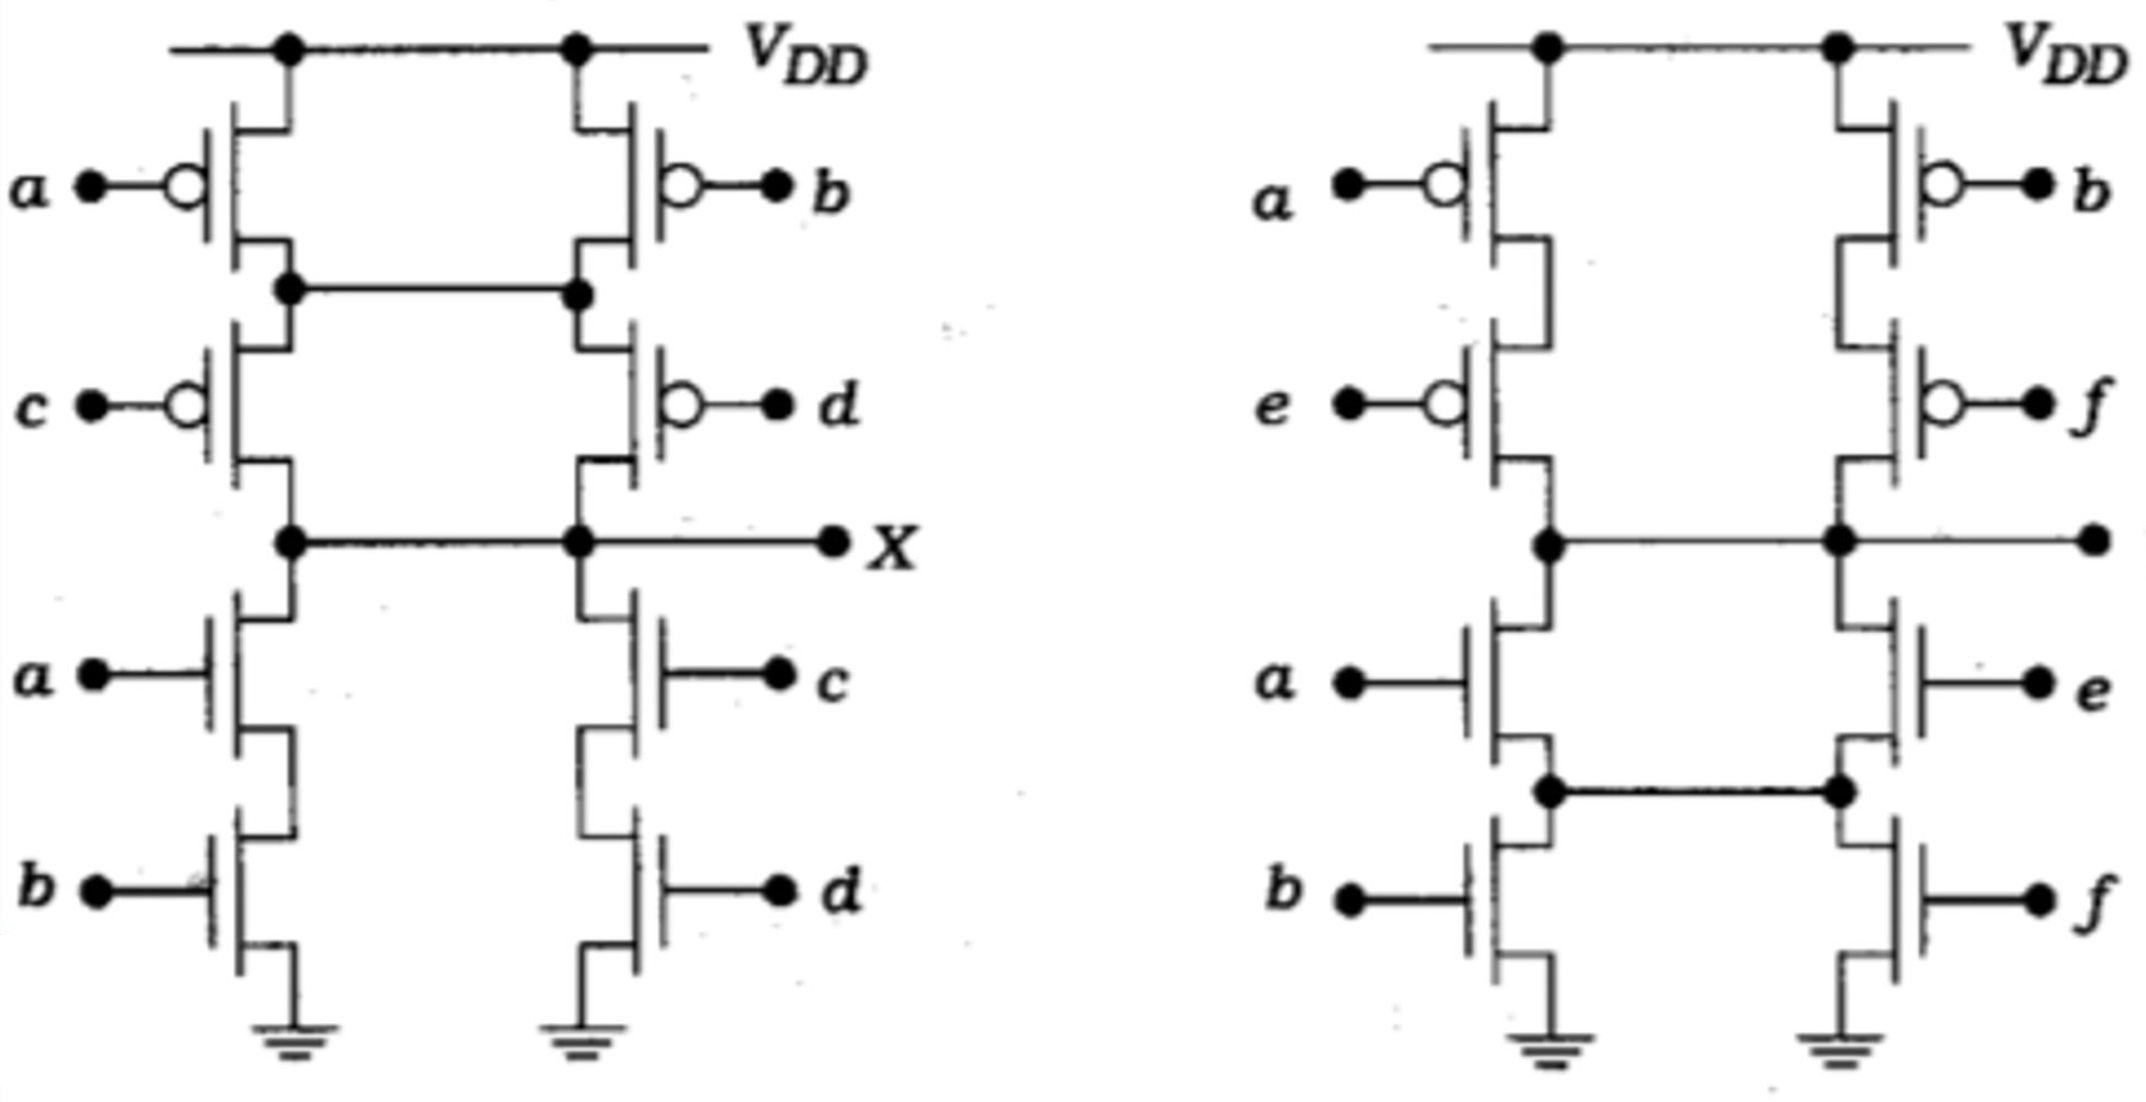
\includegraphics[width=0.5\textwidth]{aoi-oai-cmos-4-ingressi.png}
    \caption{AOI e OAI in CMOS a 4 ingressi}
    \label{fig:aoi_oai_cmos_4_ingressi}
\end{figure}

\vspace{1em}
\noindent
Per capirne la realizzazione, è sufficiente osservare che
\begin{itemize}
    \item nel caso della funzione AOI, ossia $\overline{AB+CD}$, la funzione deve produrre in uscita il valore $1$ solamente quando i suoi due ingressi sono entrambi a $0$; ma essendo tali ingressi delle porte AND, per avere $0$ in uscita bisogna che almeno uno degli ingressi sia a $0$, per cui si necessita di un parallelo di CMOS a canale-$p$ per gli ingressi $A$ e $B$, collegato in serie ad un parallelo di CMOS a canale-$p$ per gli ingressi a $C$ e $D$, collegato a $V_{dd}$. Per dualità, in pull-down si dovrà avere un parallelo di due serie a canale-$n$.
    \item nel caso della funzione OAI, ossia $\overline{(A+B) \cdot (C+D)}$, la funzione deve produrre in uscita il valore $0$ solamente quando i suoi due ingressi sono entrambi a $1$; ma essendo tali ingressi delle porte OR, per avere $1$ in uscita bisogna che almeno uno degli ingressi sia a $1$, per cui si necessita di un parallelo di CMOS a canale-$n$ per gli ingressi $A$ e $B$, collegato in serie ad un parallelo di CMOS a canale-$n$ per gli ingressi a $C$ e $D$, collegato a massa. Per dualità, in pull-up si dovrà avere un parallelo di due serie di CMOS a canale-$p$.
\end{itemize}

\vspace{1em}
\noindent
\subsubsection{Realizzazione pratica della tecnologia CMOS}
Per realizzare tali dispositivi in tecnologia CMOS, si parte dal \textbf{semiconduttore} per eccellenza, ossia il silicio:

\begin{figure}[H]
    \centering
    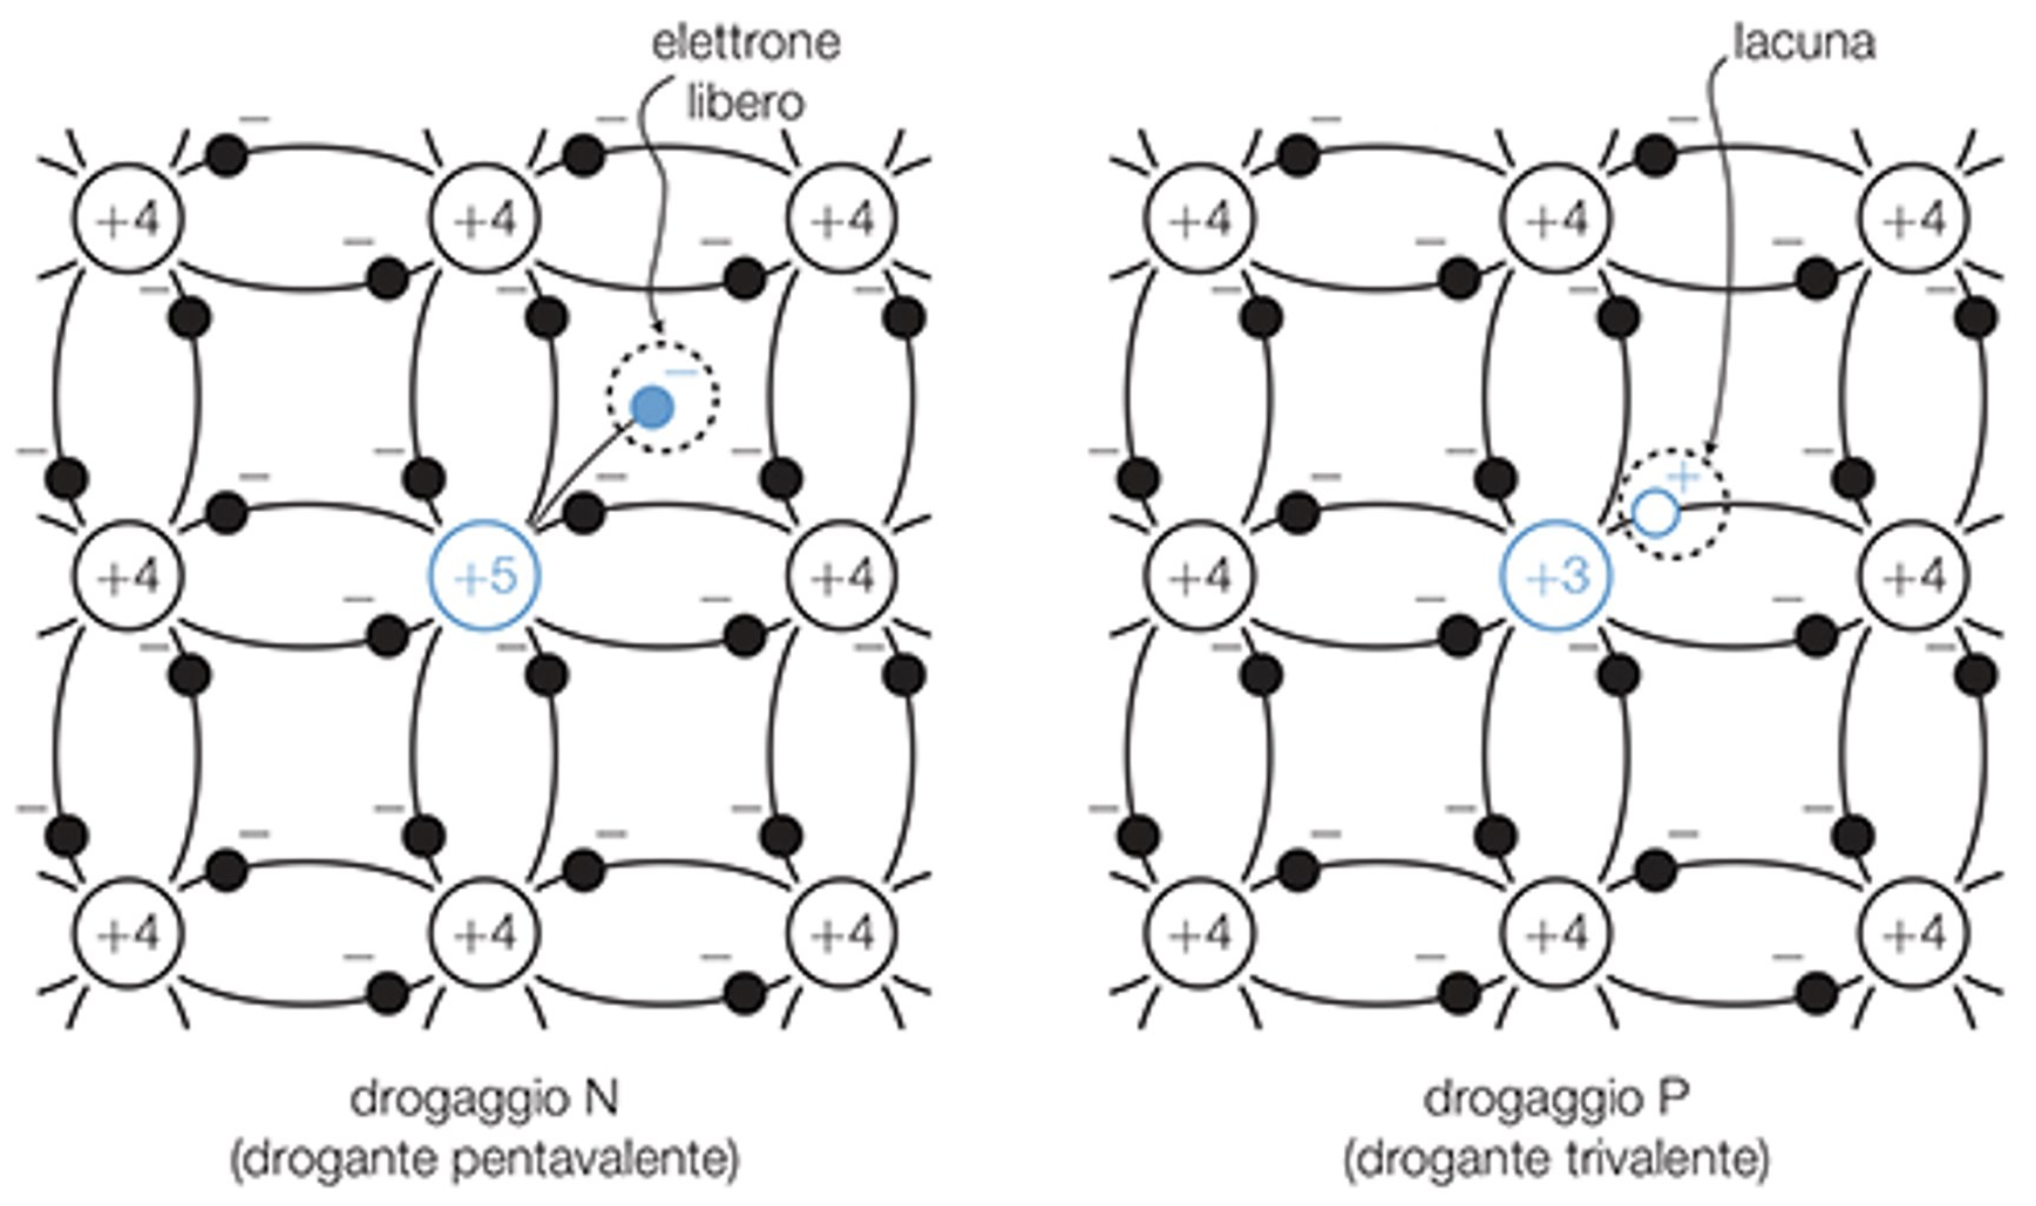
\includegraphics[width=0.6\textwidth]{semiconduttore.png}
    \caption{Silicio e relativo drogaggio}
    \label{fig:silicio_drogaggio}
\end{figure}

\noindent
Tale elemento presenta un atomo che nell'orbita più esterna presenta $4$ elettroni e si presenta naturalmente sotto-forma di reticolo; se, tramite il drogaggio, si sostituiscono alcuni atomi di silicio con altri atomi che presentano $5$ elettroni nell'orbita più esterna, l'elettrone in più non trova una sua collocazione stabile nel reticolo ed è, quindi, libero di muoversi, ottenendo un drogaggio $n$ e quindi un canale-$n$.\\
Viceversa se si sostituiscono alcuni atomi di silicio con altri atomi che presentano meno di $4$ elettroni nell'orbita più esterna, si vanno a creare dei buchi nel reticolo che prendono il nome di lacune, ottenendo un drogaggio $p$ e quindi un canale-$p$.

\vspace{1em}
\noindent
Si parte, quindi, dal silicio policristallino, chiamato anche \textbf{poli-silicio}, il quale viene inserito all'interno di un crogiolo, dopo aver subito un processo di purificazione, e viene portato a fusione.

\begin{figure}[H]
    \centering
    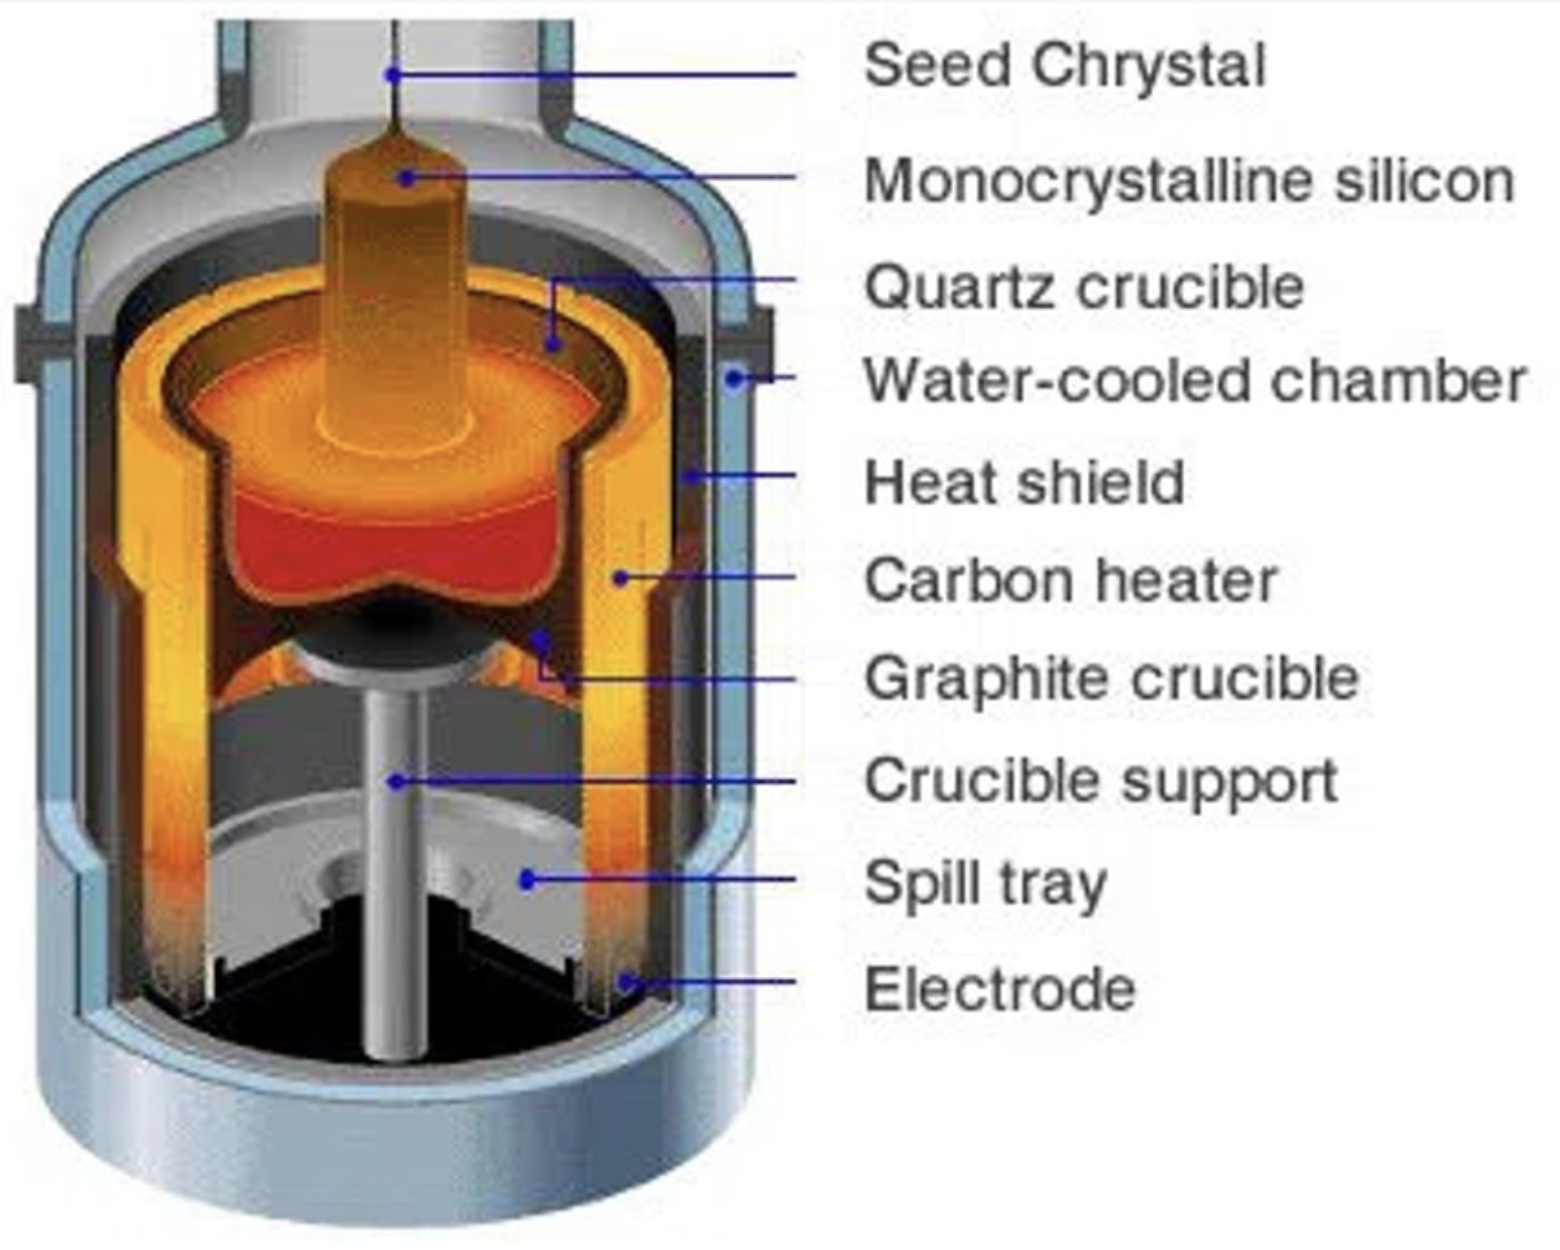
\includegraphics[width=0.4\textwidth]{estrazione-silicio-monocristallino.png}
    \caption{Estrazione del silicio monocristallino}
    \label{fig:estrazione_silicio_monocristallino}
\end{figure}

\noindent
Quando il silicio è completamente fuso vi si inserisce un seme appoggiato su un'asta rotante e, tramite una rotazione prolungata, tale seme viene lentamente estratto: a mano a mano si viene a formare un monocristallo di silicio, sotto-forma di lingotto.\\
Successivamente si seziona tale lingotto in delle sottilissime fettine, denominate \textbf{wafer}, e attraverso un processo di lappatura e lucidatura si ottiene una struttura di wafers a piani paralleli. I processi necessari per ottenere i transistor sono i seguenti
\begin{itemize}
    \item l'\textbf{ossidazione}, per fare crescere sul silicio l'ossido di silicio.
    
    \begin{figure}[H]
        \centering
        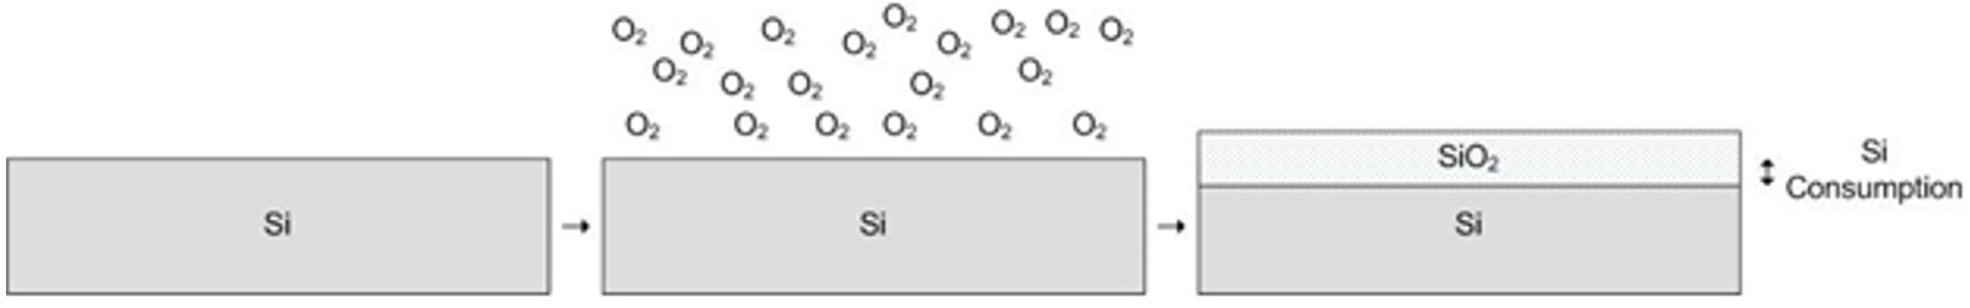
\includegraphics[width=0.6\textwidth]{ossidazione.png}
        \caption{Ossidazione}
        \label{fig:ossidazione}
    \end{figure}

    \noindent
    Tale processo prevede di inserire il wafer di silicio, previo riscaldamento ad un'opportuna temperatura, all'interno di un'atmosfera ricca di ossigeno, o di vapor acqueo, a seconda che il processo sia a secco o a umido, e sul silicio, a poco a paco, si forma uno strato di \textbf{ossido di silicio}.

    \item la \textbf{fotolitografia}, la quale sfrutta la fotografia analogica attraverso il negativo e la proiezione dell'immagine su un materiale fotosensibile.
    
    \begin{figure}[H]
        \centering
        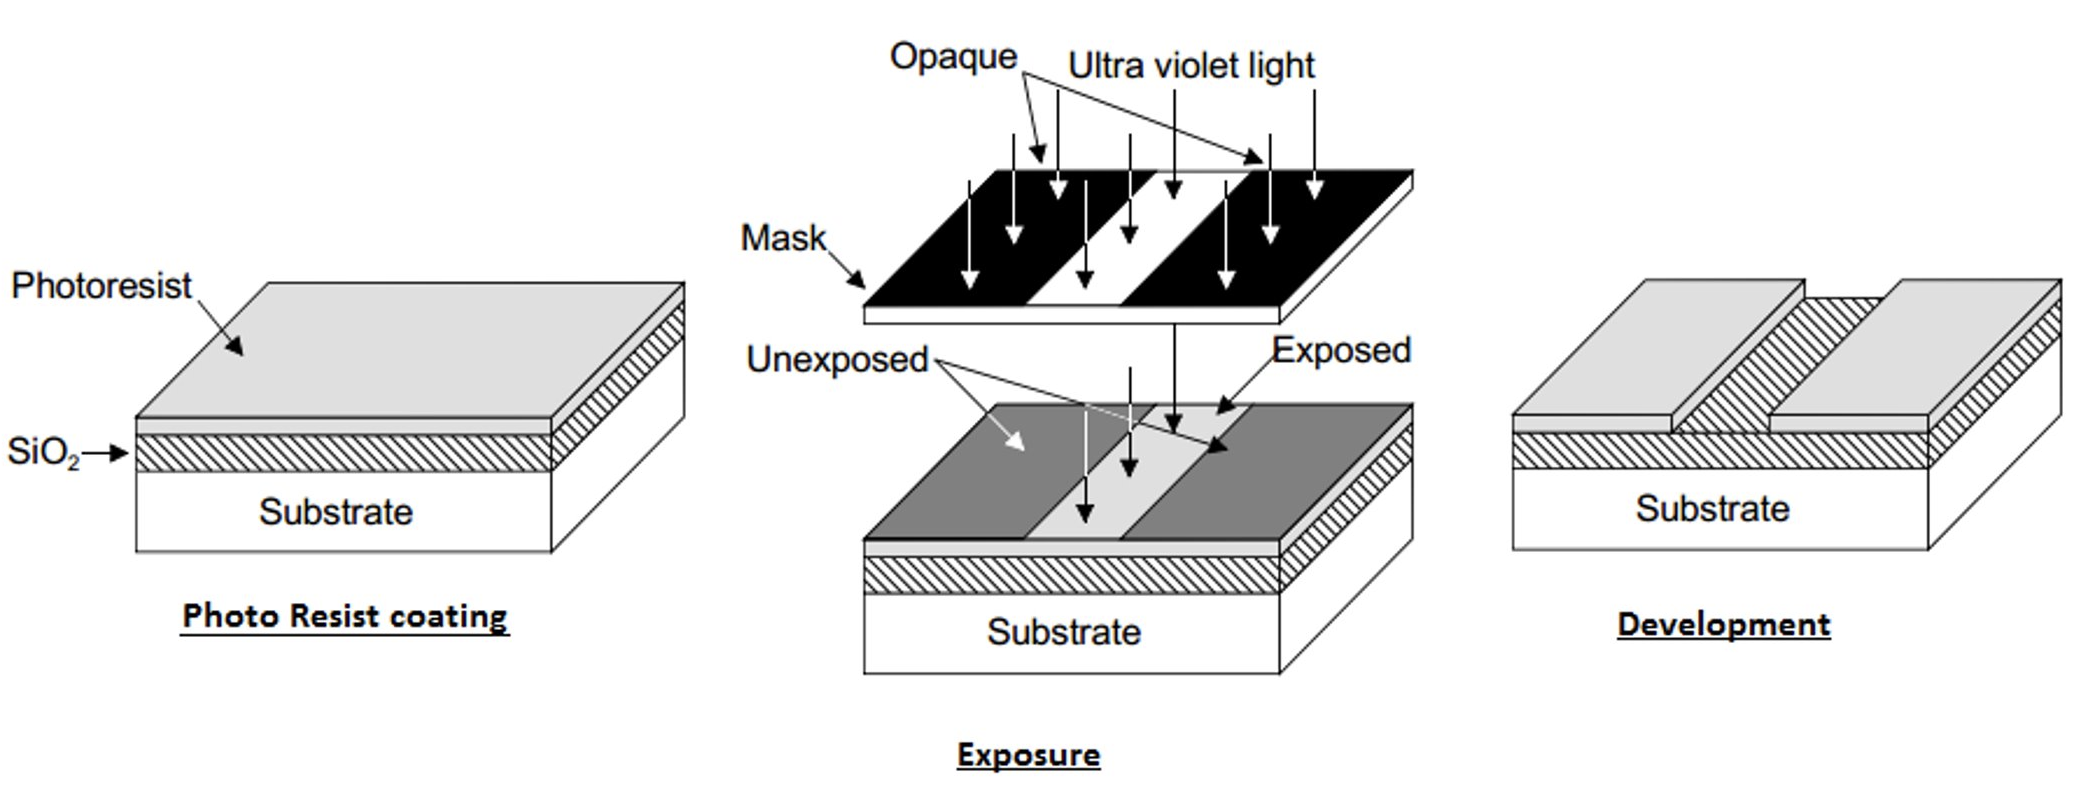
\includegraphics[width=0.6\textwidth]{fotolitografia.png}
        \caption{Fotolitografia}
        \label{fig:fotolitografia}
    \end{figure}

    \noindent
    Sopra il silicio, sul quale è cresciuto l'ossido di silicio, fatto ruotare opportunamente, viene fatto colare del foto-resist (materiale particolarmente fotosensibile), sotto-forma di goccioline; con la rotazione, il foto-resist si distribuisce su tutto il substrato e lo si fa asciugare.\\
    Una volta asciugato si impiega un negativo, simile a quello fotografico, e attraverso una luce ultravioletta si modifica la struttura del foto-resist che polimerizzerà in modo opportuno, tale da essere sviluppato. Da ultimo, tramite degli acidi, viene rimosso tutto il foto-resist che non è stata sensibilizzata, in modo tale da creare delle zone mascherate e delle zone aperte.

    \item l'\textbf{incisione (etching)} del silicio.
    
    \begin{figure}[H]
        \centering
        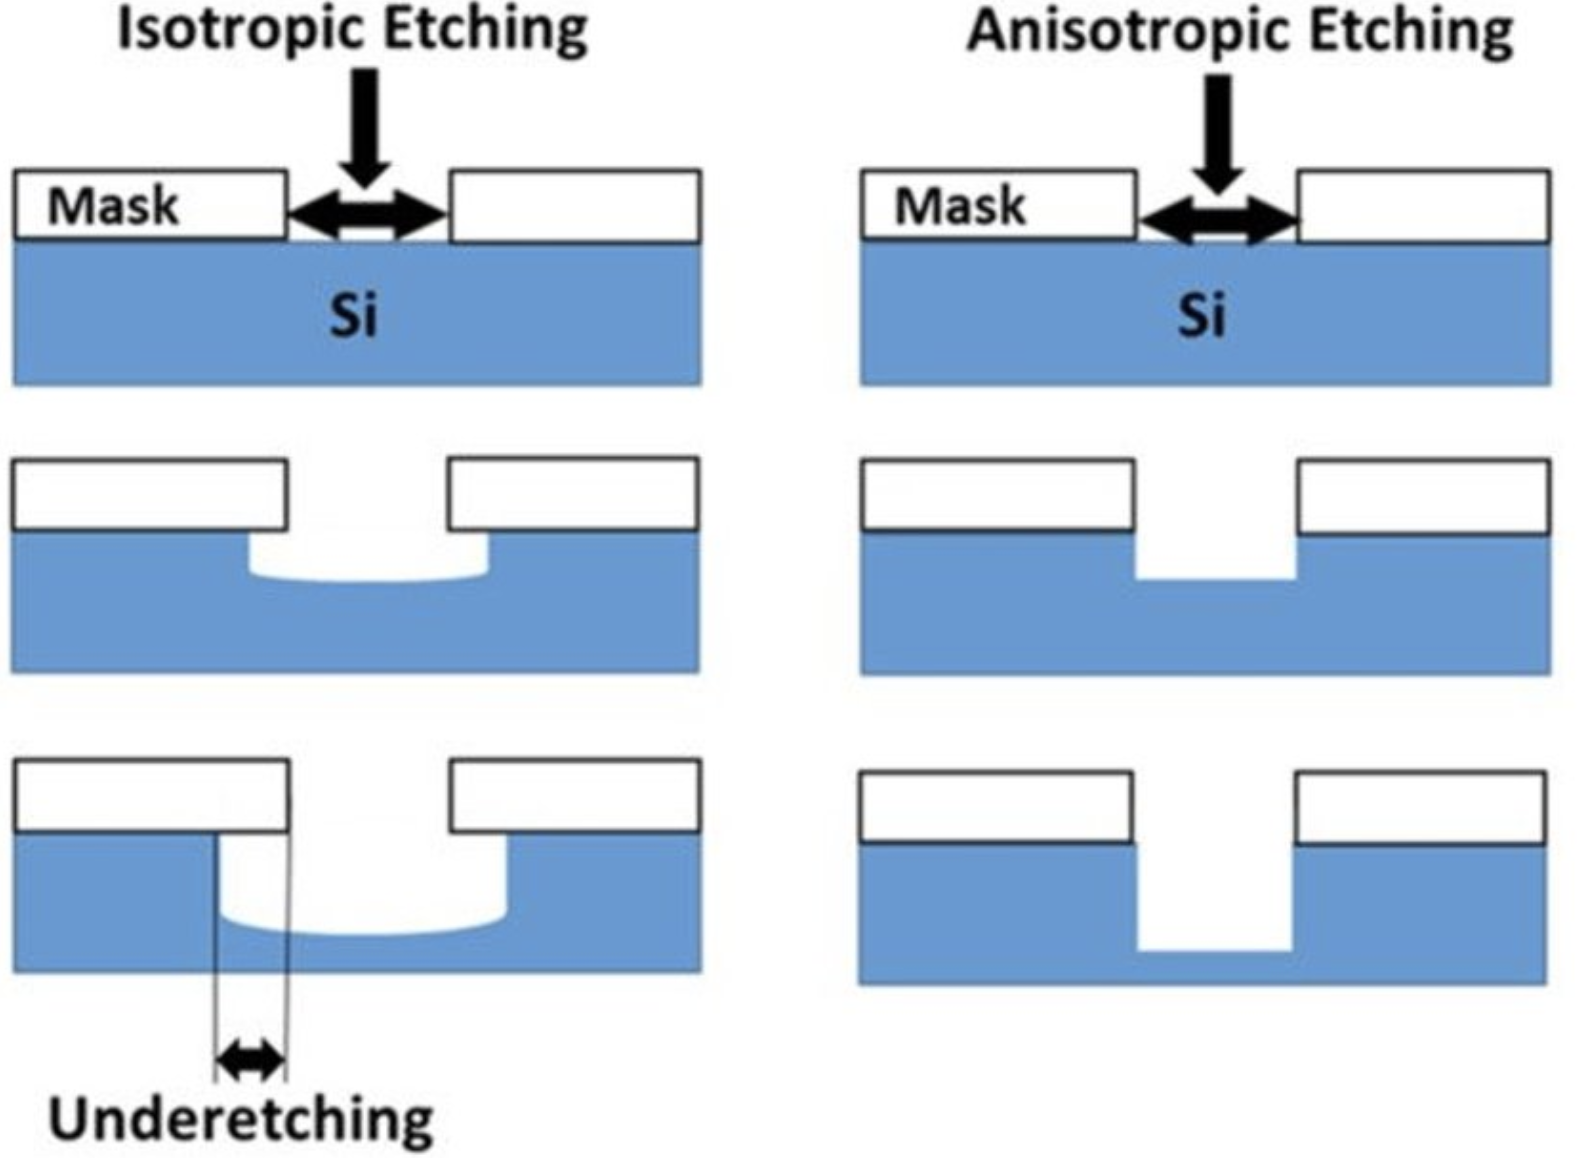
\includegraphics[width=0.5\textwidth]{etching.png}
        \caption{Etching}
        \label{fig:etching}
    \end{figure}

    \noindent
    Sfruttando il foto-resist rimasto integro, si individuano le zone non protette sulle quali si andrà ad escavare (etching) tramite acidi, plasma o altro, in maniera non molto dissimile ad un processo di sviluppo o stampa fotografica.\\
    Vi sono processi iso-tropici che prevedono un'escavazione globalmente generalizzata su tutto il silicio, oppure processi an-iso-tropici, in genere eseguiti tramite plasma, che creano delle isole nel silicio con bordi verticali.

    \item l'eventuale \textbf{deposizione} di altro materiale.
    
    \begin{figure}[H]
        \centering
        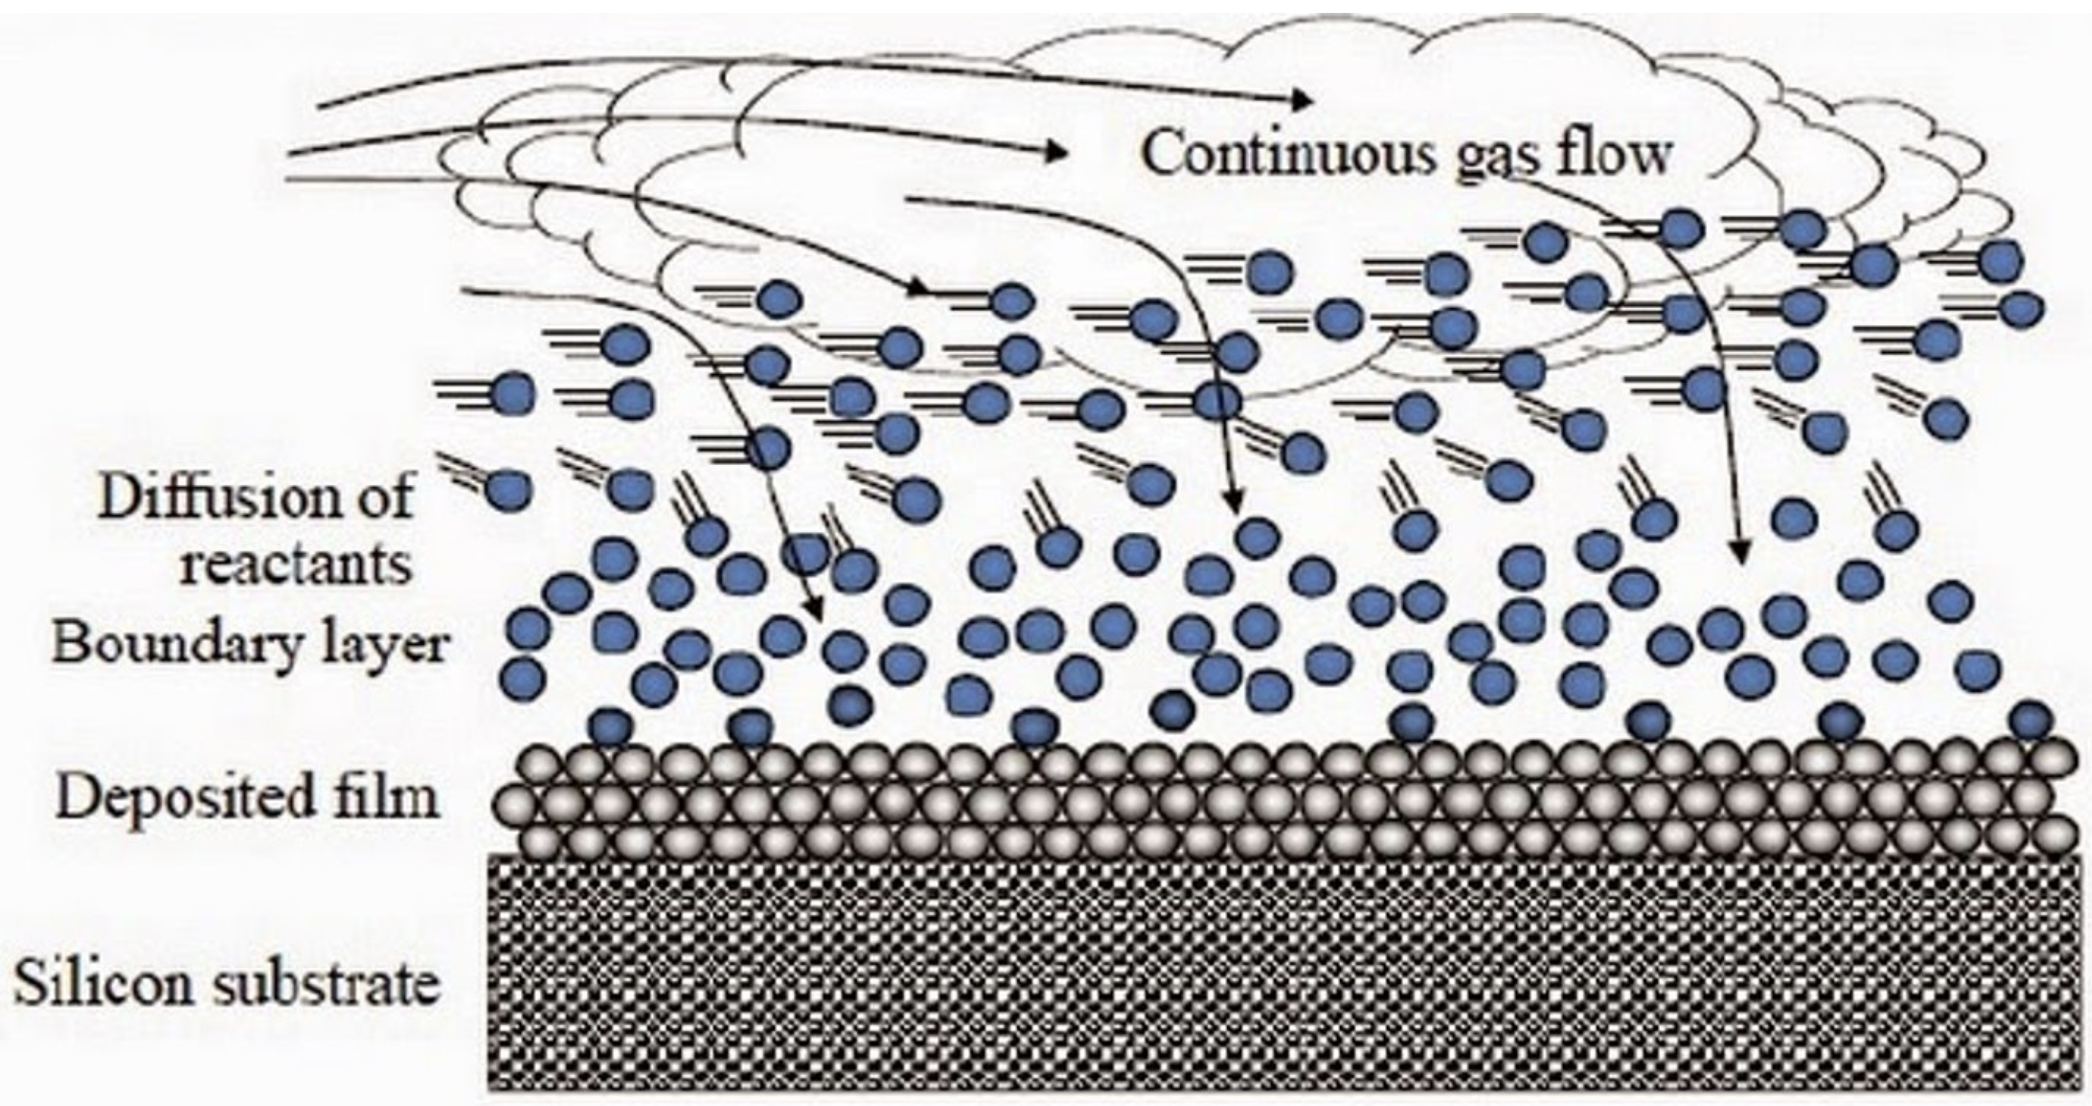
\includegraphics[width=0.5\textwidth]{deposizione.png}
        \caption{Deposizione}
        \label{fig:deposizione}
    \end{figure}

    \noindent
    Se durante la lavorazione si rende necessario depositare dell'ulteriore materiale sul silicio, si pone il silicio all'interno di un flusso costante di gas, di diversa natura, caricato opportunamente in condizioni di temperatura e pressione controllate, per far sì che tali particelle possano depositarsi sul silicio e creare un film sul silicio stesso.

    \item l'\textbf{impiantazione ionica} e la \textbf{ricottura (annealing)} del silicio.
    
    \begin{figure}[H]
        \centering
        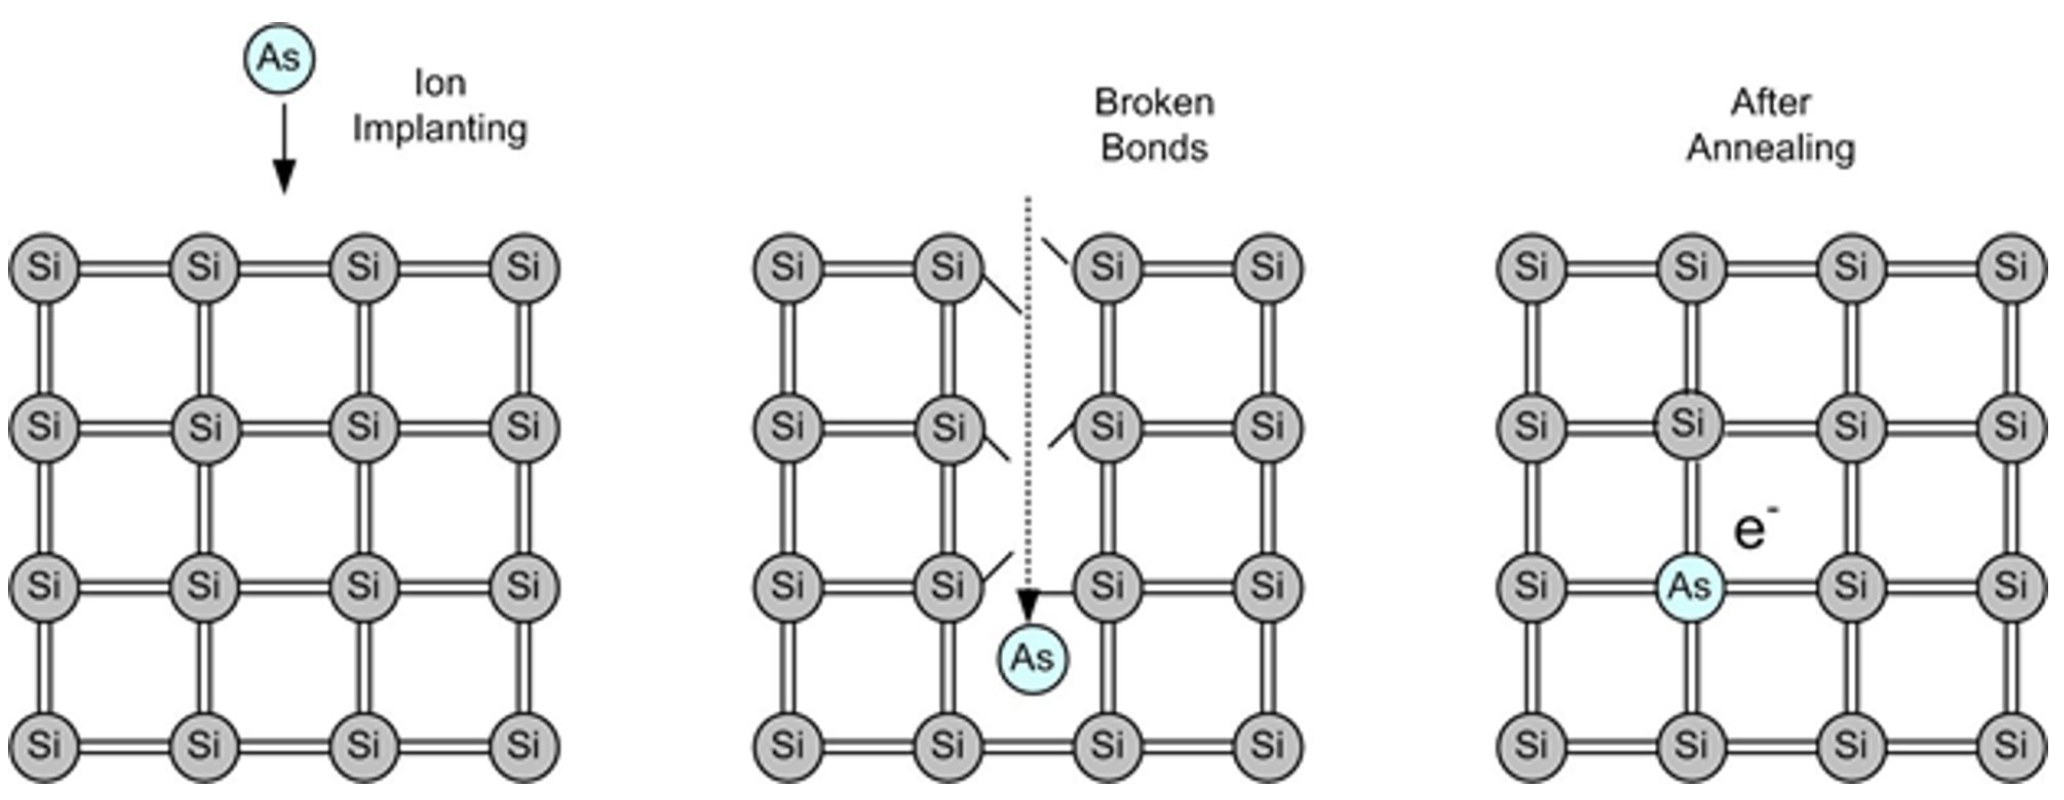
\includegraphics[width=0.6\textwidth]{impiantazione-ionica-ricottura.png}
        \caption{Impiantazione ionica e ricottura}
        \label{fig:impiantazione_ionica_ricottura}
    \end{figure}

    \noindent
    Tramite l'impiantazione ionica vengono sparati degli ioni di materiali opportuni, come ioni di materiali droganti; a seconda del campo elettrico tali ioni penetrano più o meno profondamente all'interno del silicio, spaccando i legami del silicio; successivamente, tuttavia, tramite una ricottura, riscaldando nuovamente il silicio, i legami si riassestano e gli ioni impiantati trovano la loro regolare ubicazione all'interno del reticolo.
\end{itemize}

\vspace{1em}
\noindent
\subsubsection{Fabbricazione di un invertitore in tecnologia CMOS}
Com'è noto, un invertitore CMOS è un dispositivo realizzato mediante un transistor a canale-$p$ e un transistor a canale-$n$, opportunamente collegati fra loro.\\
Innanzitutto, si creano delle zone isolate all'interno del silicio e delle zone di isolamento realizzato mediante l'ossido di silicio poste sopra il silicio; in questo modo si ottiene il wafer mostrato in Figura \ref{fig:fabbricazione_invertitore_cmos_1}, tutto di una tipologia, solitamente di tipologia $p$, quindi con eccedenza di lacune, ma in essa viene creata una zona drogata $n$ (chiamata $n$-well), nella quale realizzare i transistor a canale-$p$, ricco di cariche negative.

\begin{figure}[H]
    \centering
    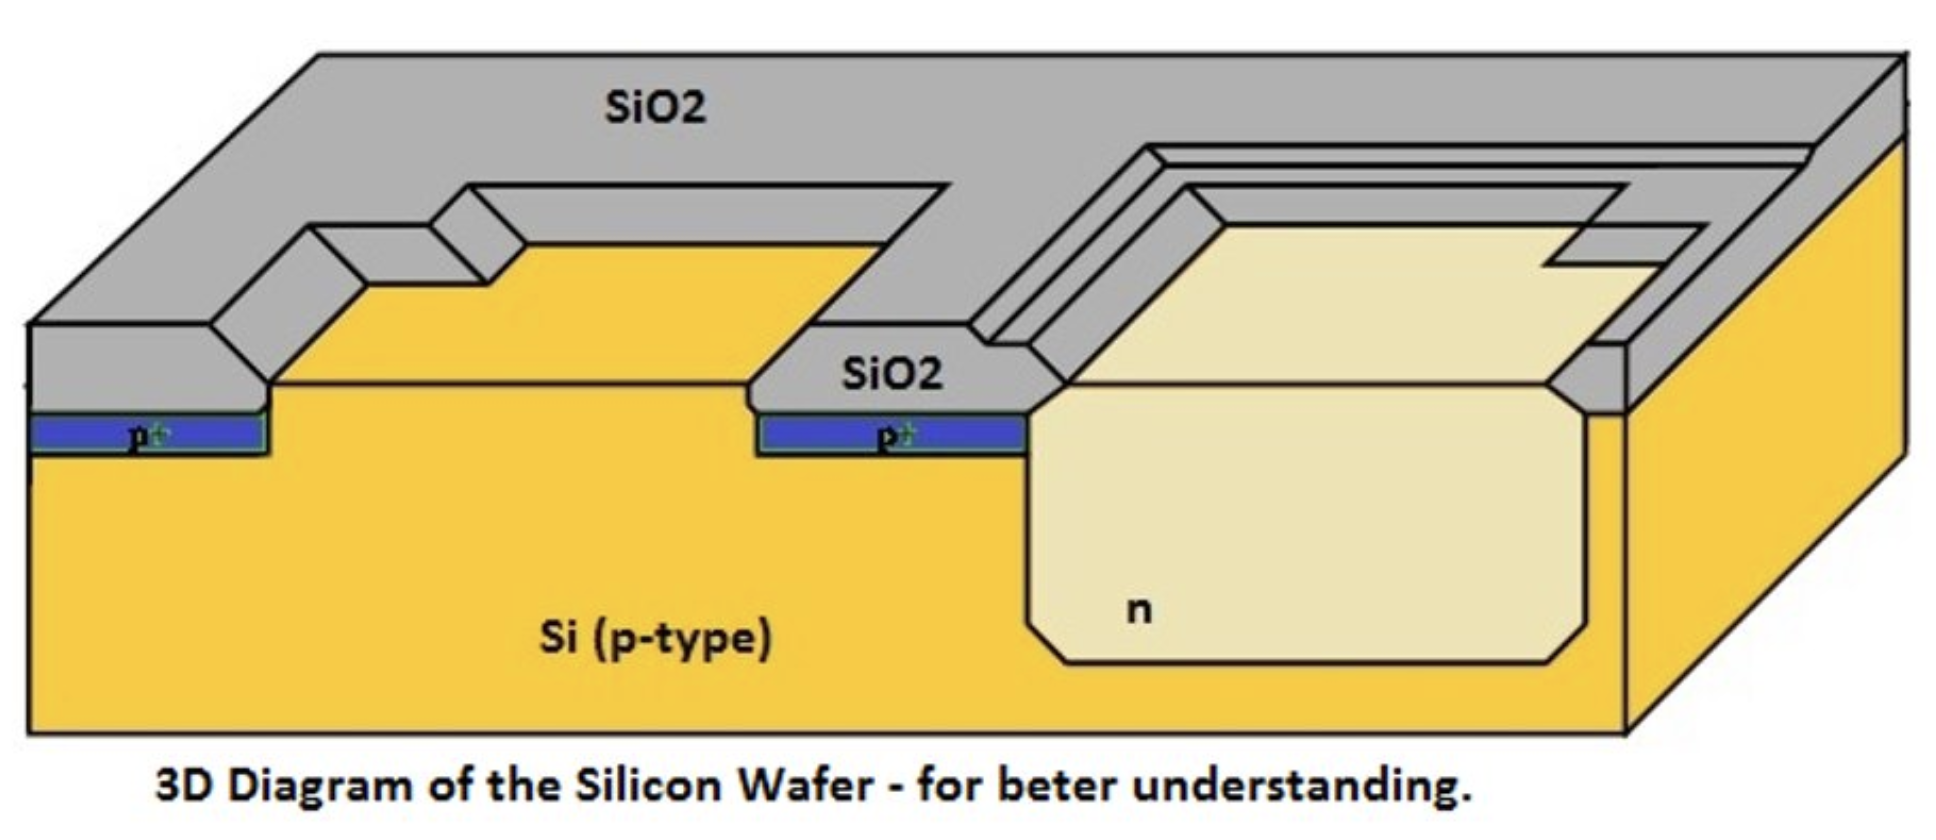
\includegraphics[width=0.5\textwidth]{fabbricazione-invertitore-cmos-1.png}
    \caption{Fabbricazione di un invertitore in tecnologia CMOS - Fase 1}
    \label{fig:fabbricazione_invertitore_cmos_1}
\end{figure}

\noindent
Successivamente su tale wafer si fa crescere un sottilissimo strato di ossido che serve da isolante per la realizzazione del canale, come mostrato nella figura seguente.

\begin{figure}[H]
    \centering
    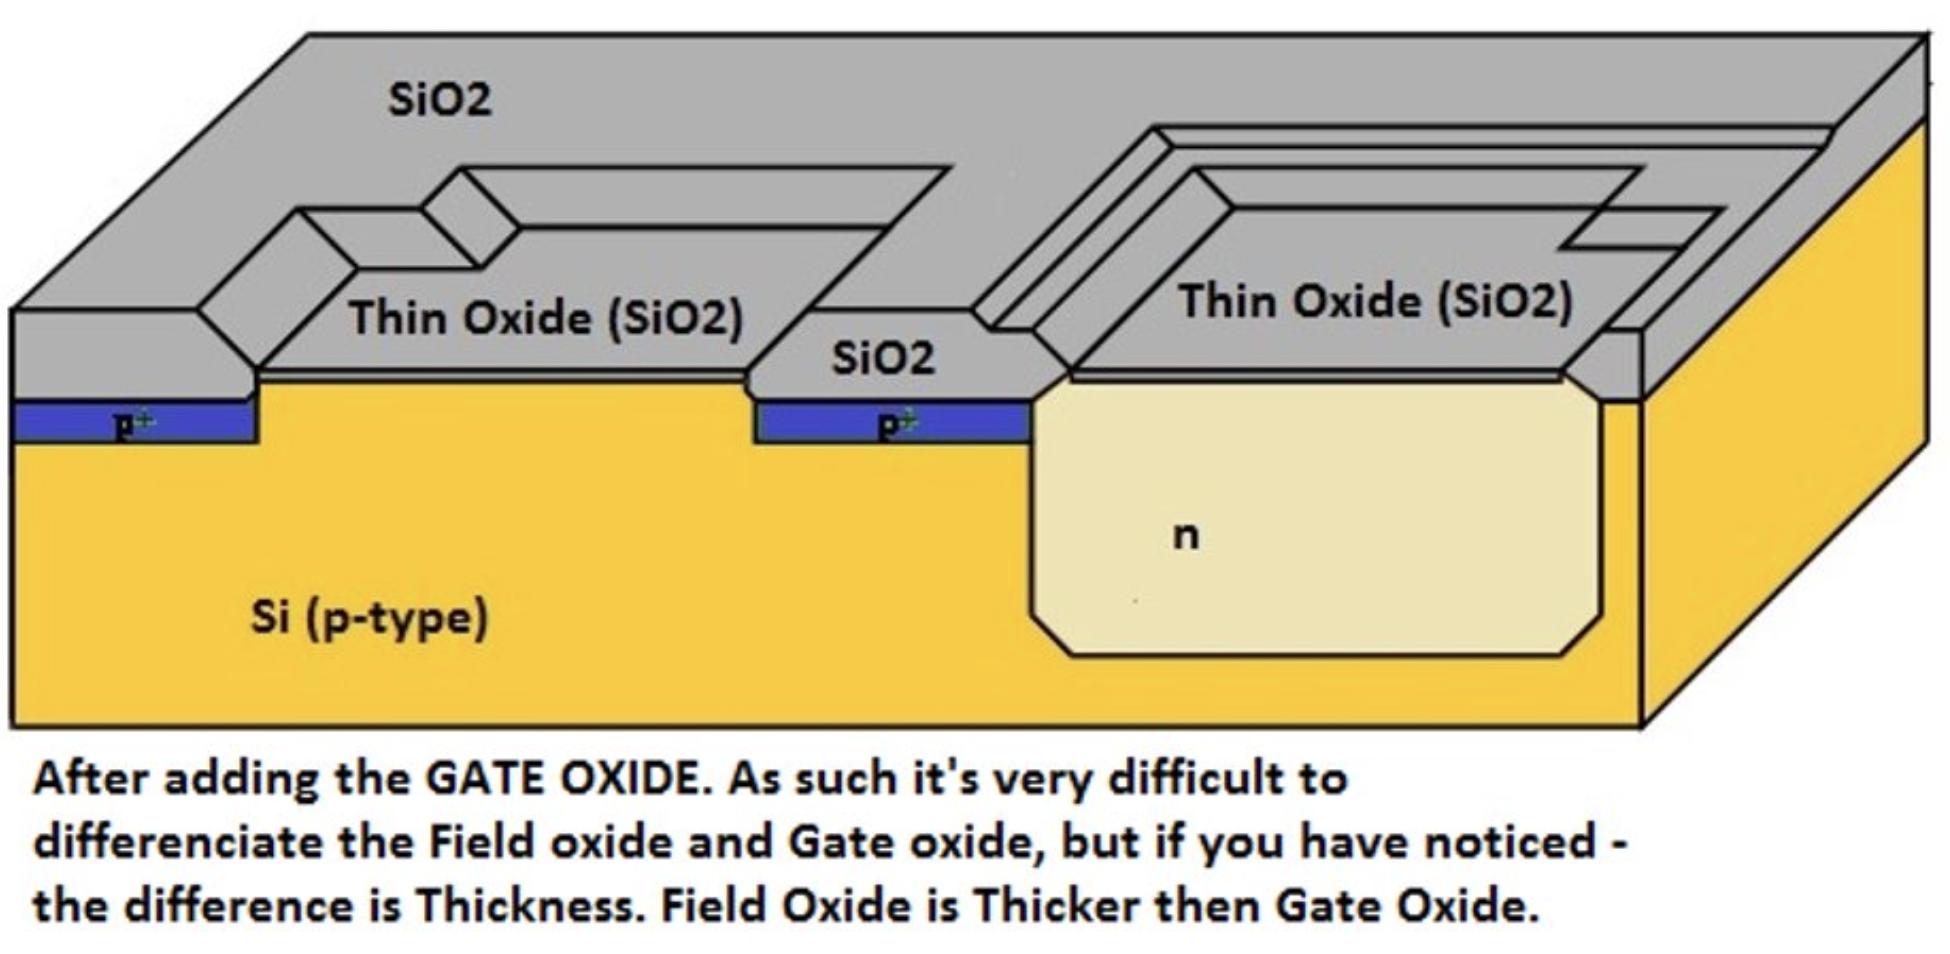
\includegraphics[width=0.5\textwidth]{fabbricazione-invertitore-cmos-2.png}
    \caption{Fabbricazione di un invertitore in tecnologia CMOS - Fase 2}
    \label{fig:fabbricazione_invertitore_cmos_2}
\end{figure}

\noindent
Dopodiché si elimina lo strato di silicio laddove non serve e si fa crescere sopra tale substrato di silicio del silicio poli-cristallino che funge da conduttore, nonché da gate al di sopra dei transistor

\begin{figure}[H]
    \centering
    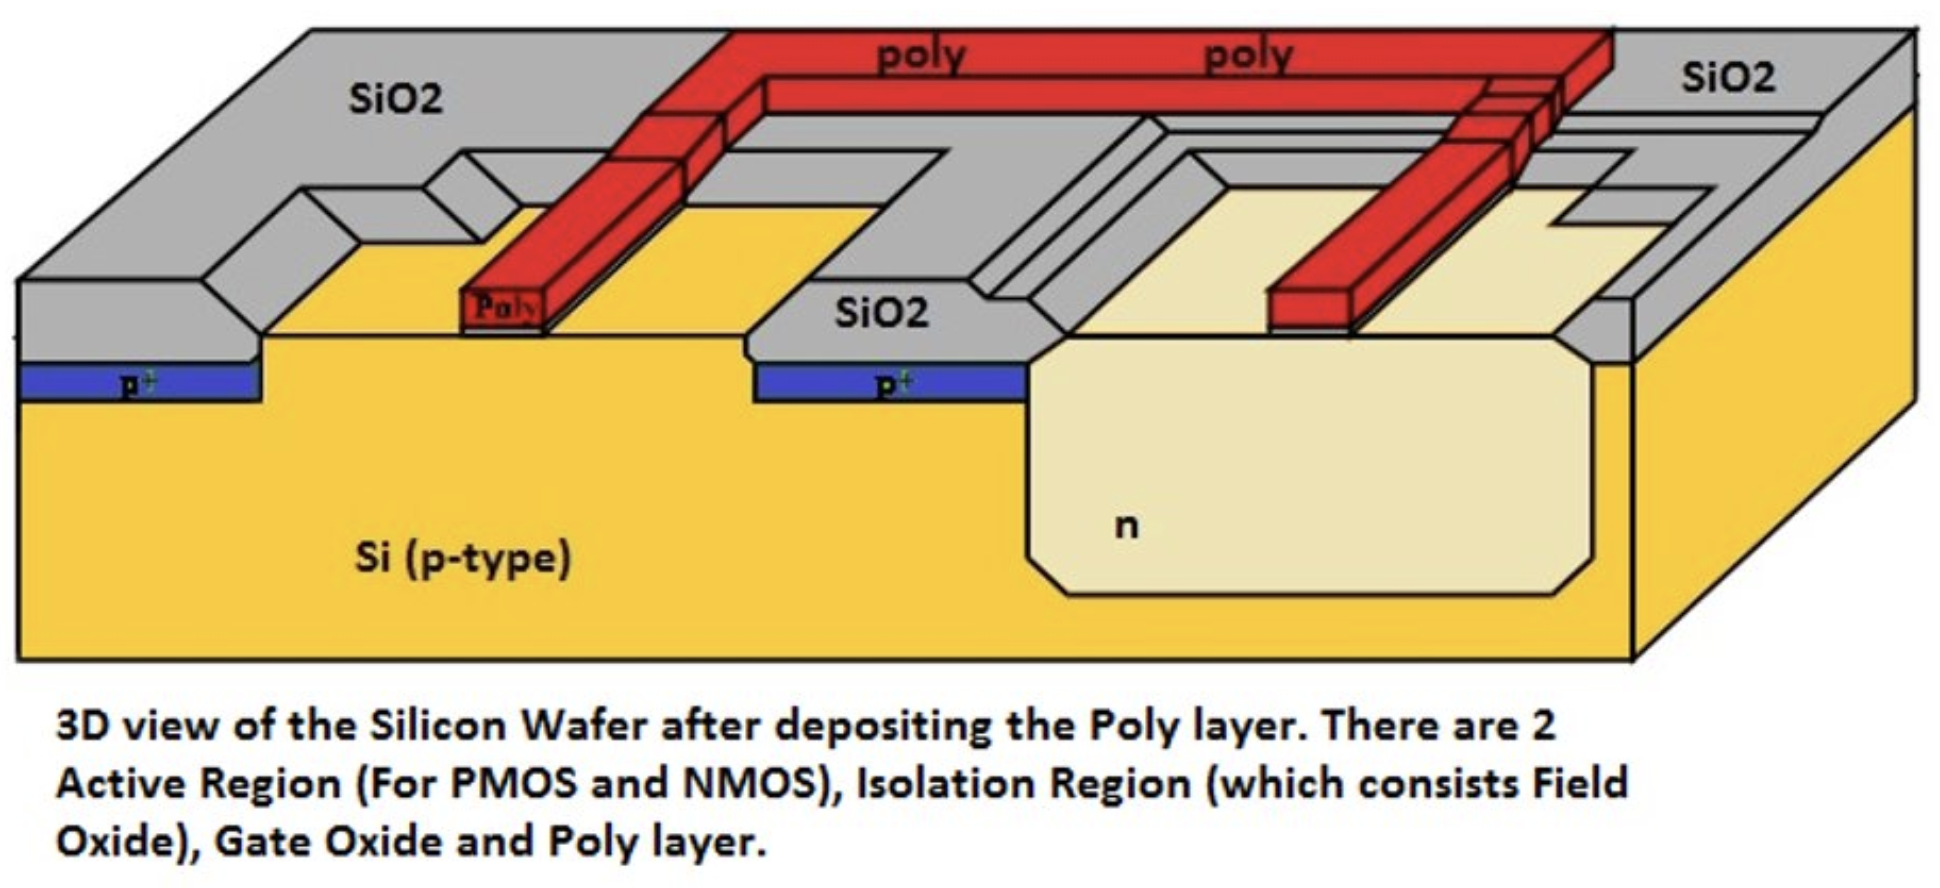
\includegraphics[width=0.5\textwidth]{fabbricazione-invertitore-cmos-3.png}
    \caption{Fabbricazione di un invertitore in tecnologia CMOS - Fase 3}
    \label{fig:fabbricazione_invertitore_cmos_3}
\end{figure}

\noindent
Dopo aver realizzato il silicio poli-cristallino si crea, tramite impiantazione ionica, un drogaggio $n$ nel substrato $p$ e un drogaggio $p$ nel substrato $n$:

\begin{figure}[H]
    \centering
    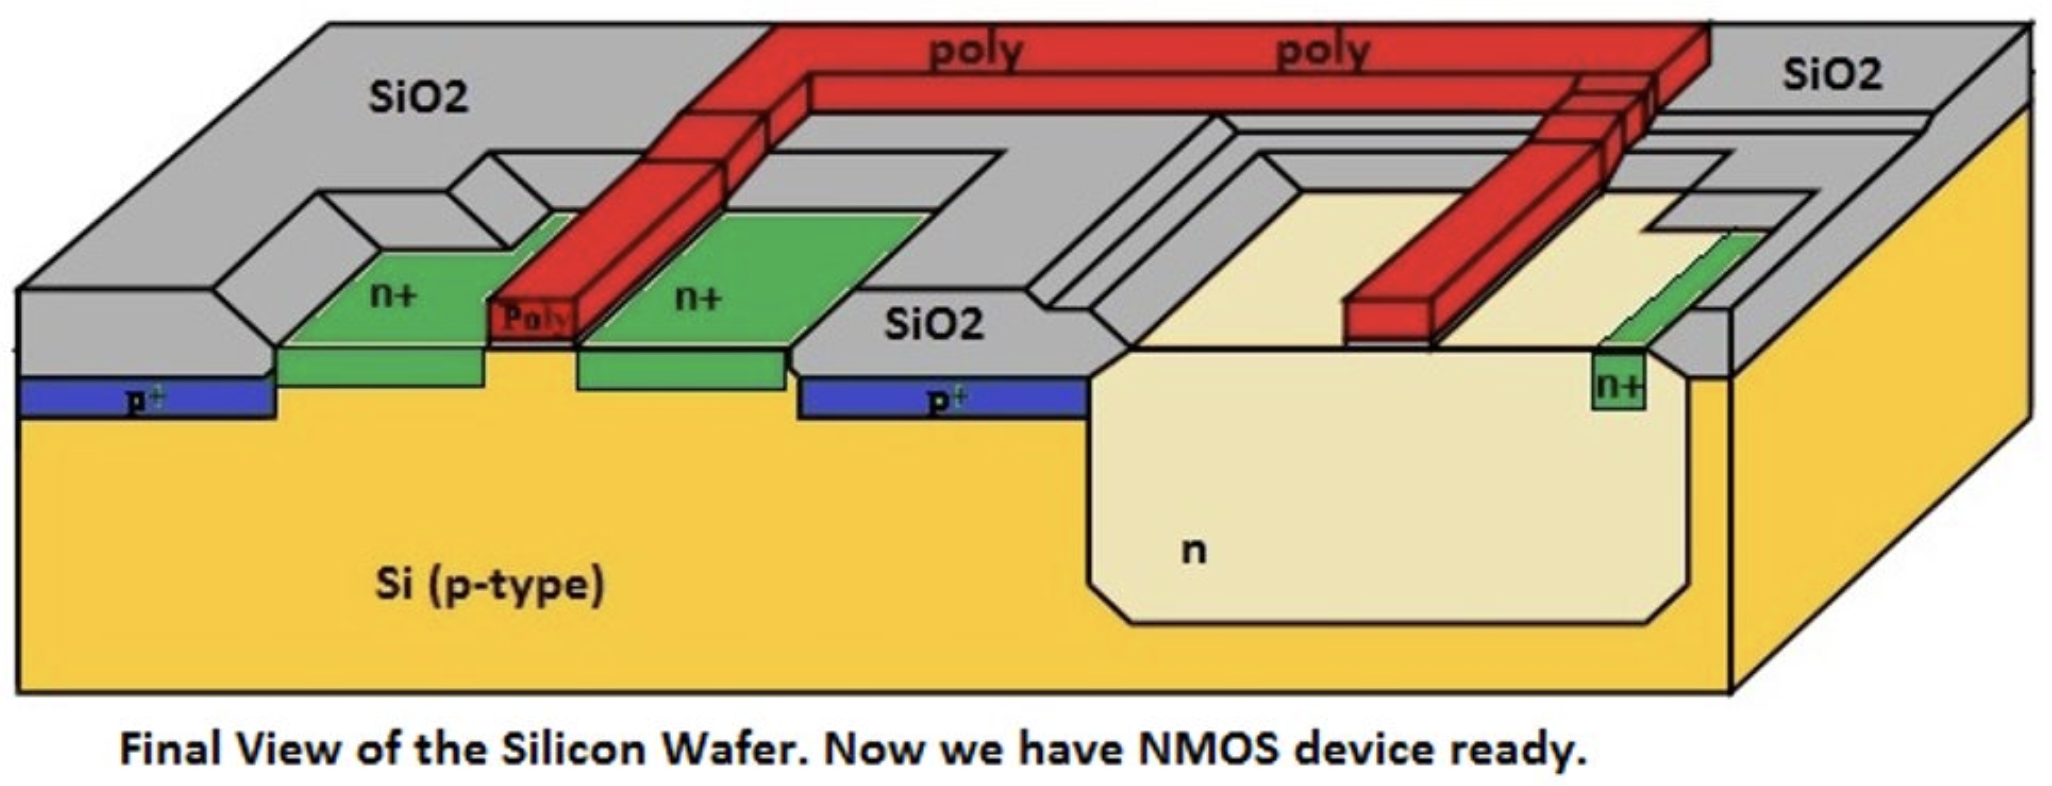
\includegraphics[width=0.5\textwidth]{fabbricazione-invertitore-cmos-4.png}
    \caption{Fabbricazione di un invertitore in tecnologia CMOS - Fase 4}
    \label{fig:fabbricazione_invertitore_cmos_4}
\end{figure}

\noindent
Finalmente, quindi, sono stati ottenuti i due transistor: in mezzo rimarrà aperto il canale che si chiuderà elettricamente quando si forniranno le tensioni opportune:

\begin{figure}[H]
    \centering
    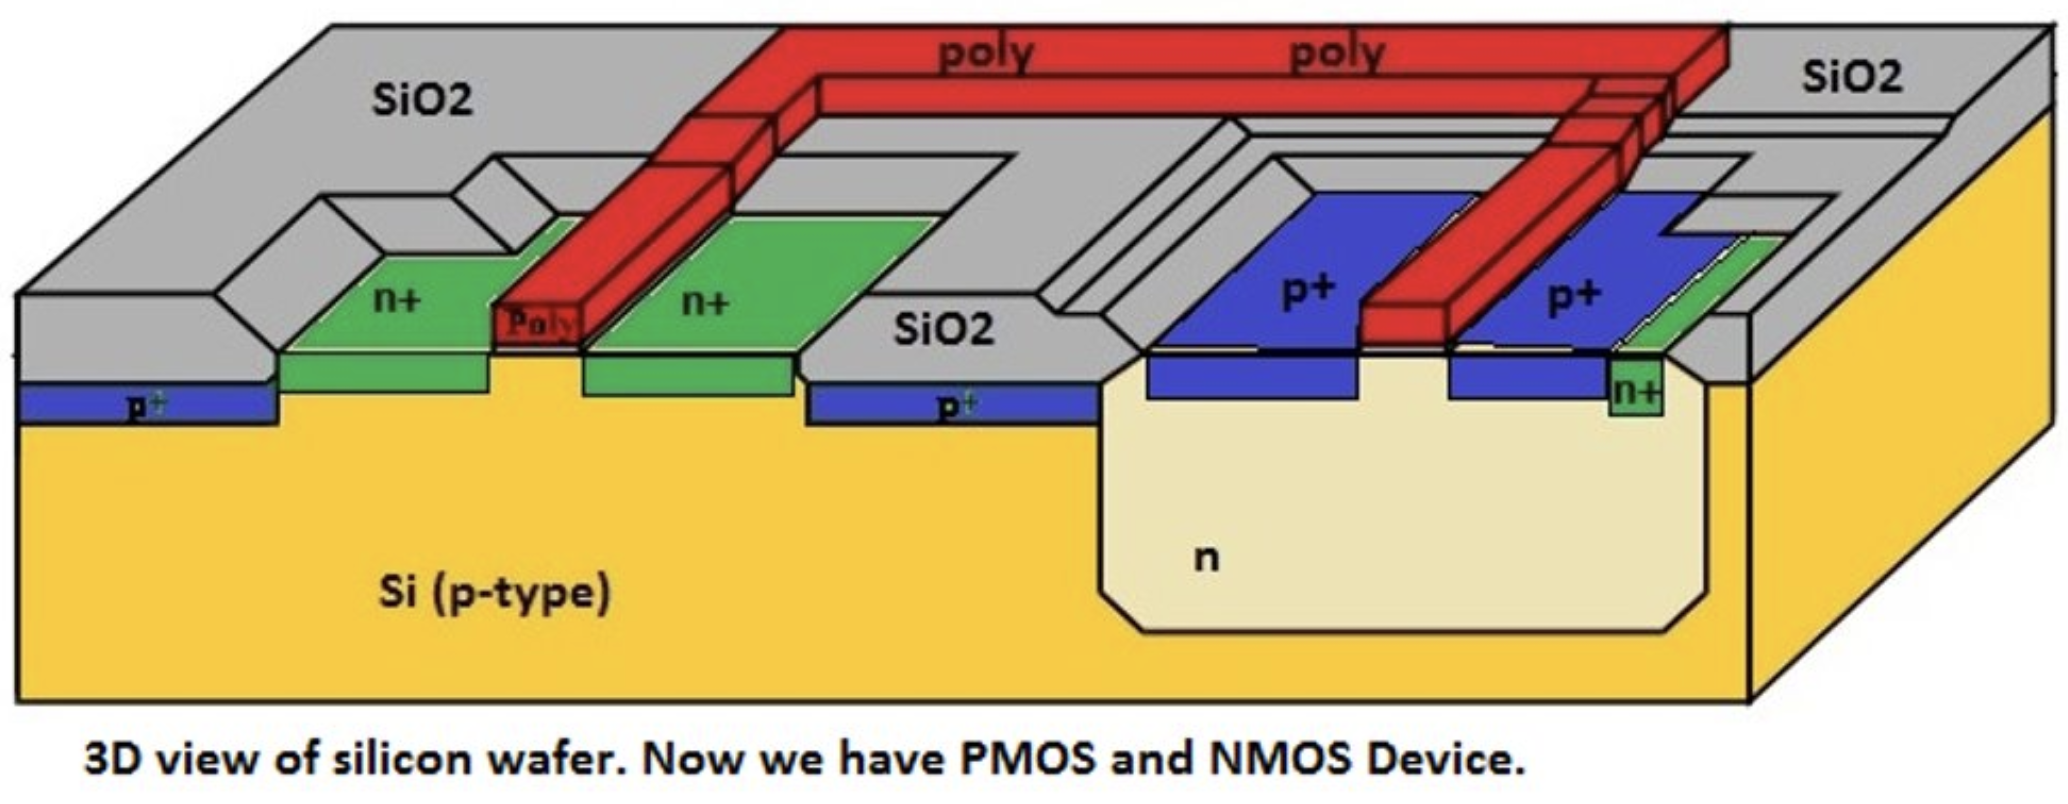
\includegraphics[width=0.5\textwidth]{fabbricazione-invertitore-cmos-5.png}
    \caption{Fabbricazione di un invertitore in tecnologia CMOS - Fase 5}
    \label{fig:fabbricazione_invertitore_cmos_5}
\end{figure}

\noindent
Infine, al di sopra di tutto, vengono create le metallizzazioni che vanno ad instaurare il collegamento tra i punti di contatto necessari:

\begin{figure}[H]
    \centering
    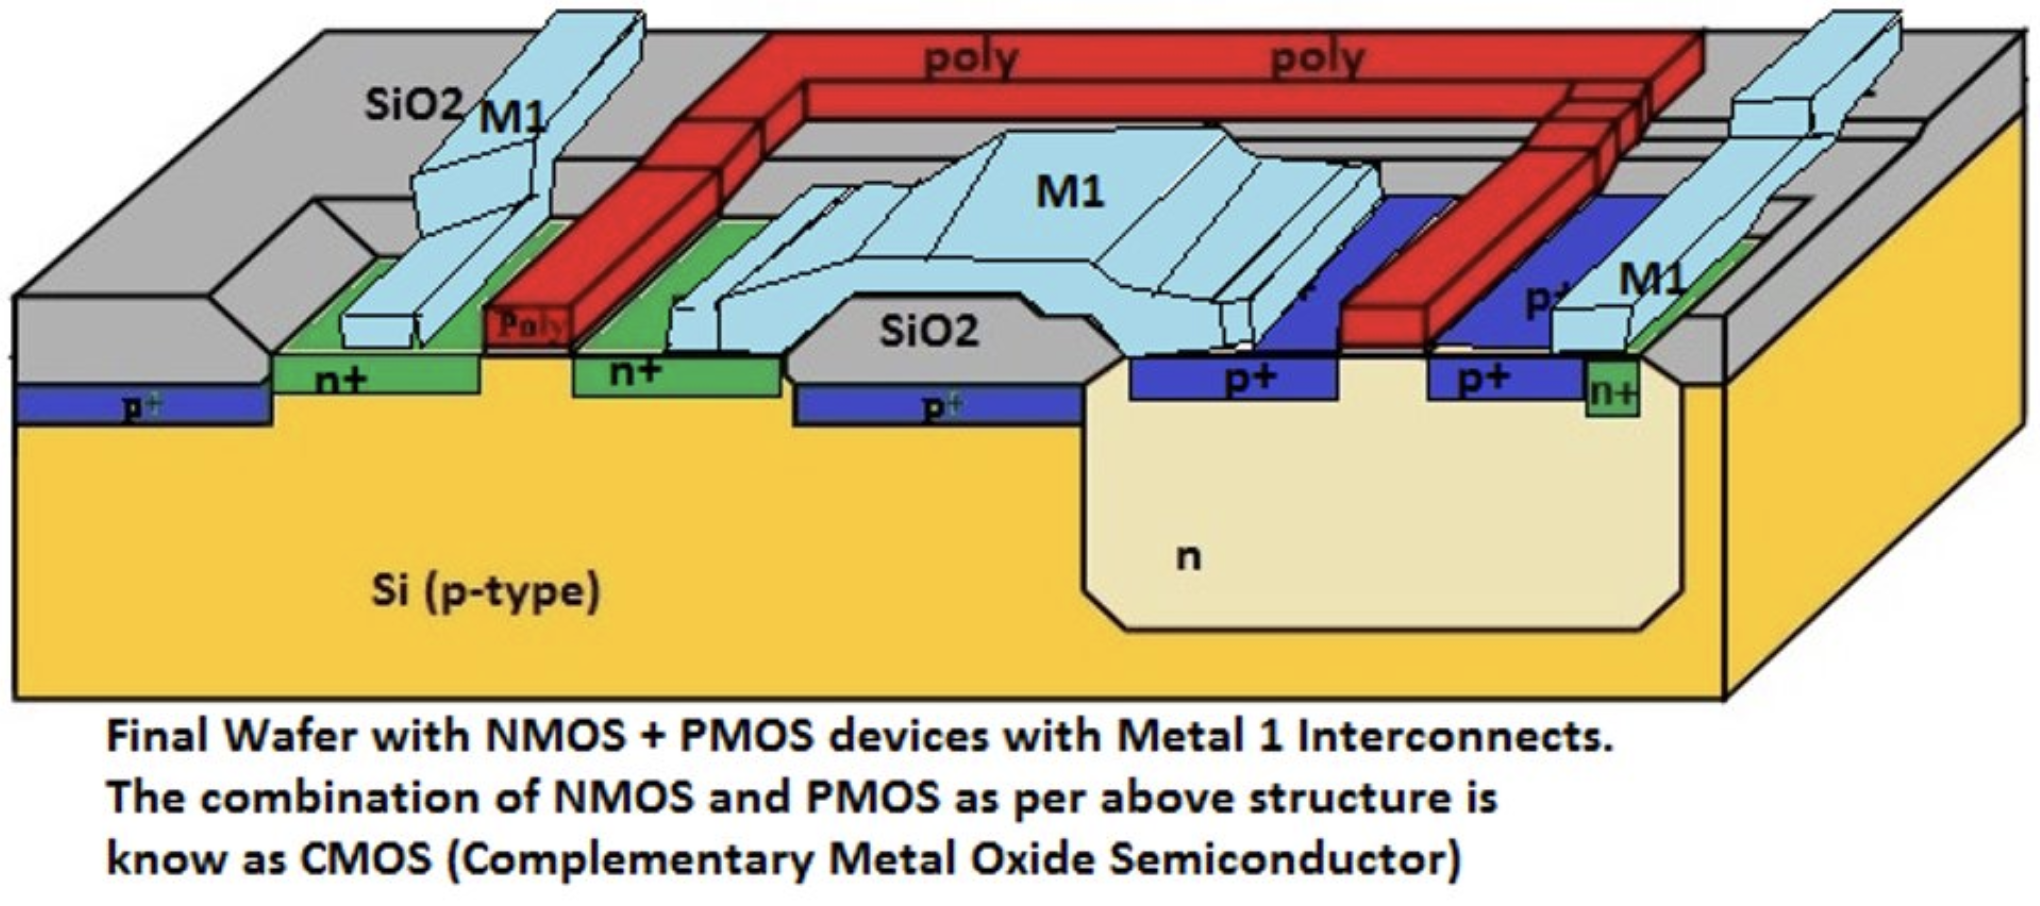
\includegraphics[width=0.5\textwidth]{fabbricazione-invertitore-cmos-6.png}
    \caption{Fabbricazione di un invertitore in tecnologia CMOS - Fase 6}
    \label{fig:fabbricazione_invertitore_cmos_6}
\end{figure}

\vspace{1em}
\noindent
Ecco che quindi si è ottenuto l'invertitore in tecnologia CMOS desiderato, con un numero di fasi pari a $73$, di gran lunga superiori rispetto alle sole $6$ schematizzate in precedenza.

\vspace{1em}
\noindent
\textbf{Osservazione}: Per passare dai collegamenti al Layout su Silicio si può far uso dello \textbf{Stick Diagram}. Esso, in particolare
\begin{itemize}
    \item mostra la topografia del circuito;
    \item mostra i componenti ed i contatti;
    \item mostra la posizione relativa dei componenti;
    \item aiuta a progettare il layout e i collegamenti.
\end{itemize}
Tuttavia
\begin{itemize}
    \item non mostra il posizionamento esatto;
    \item non mostra le dimensioni finali dei transistor;
    \item non mostra le dimensioni (larghezza e lunghezza dei collegamenti);
    \item non mostra altri dettagli quali effetti parassiti (resistenze, capacità, etc.).
\end{itemize}
Per la rappresentazione, pertanto, si ricorre alla convenzione seguente

\begin{figure}[H]
    \centering
    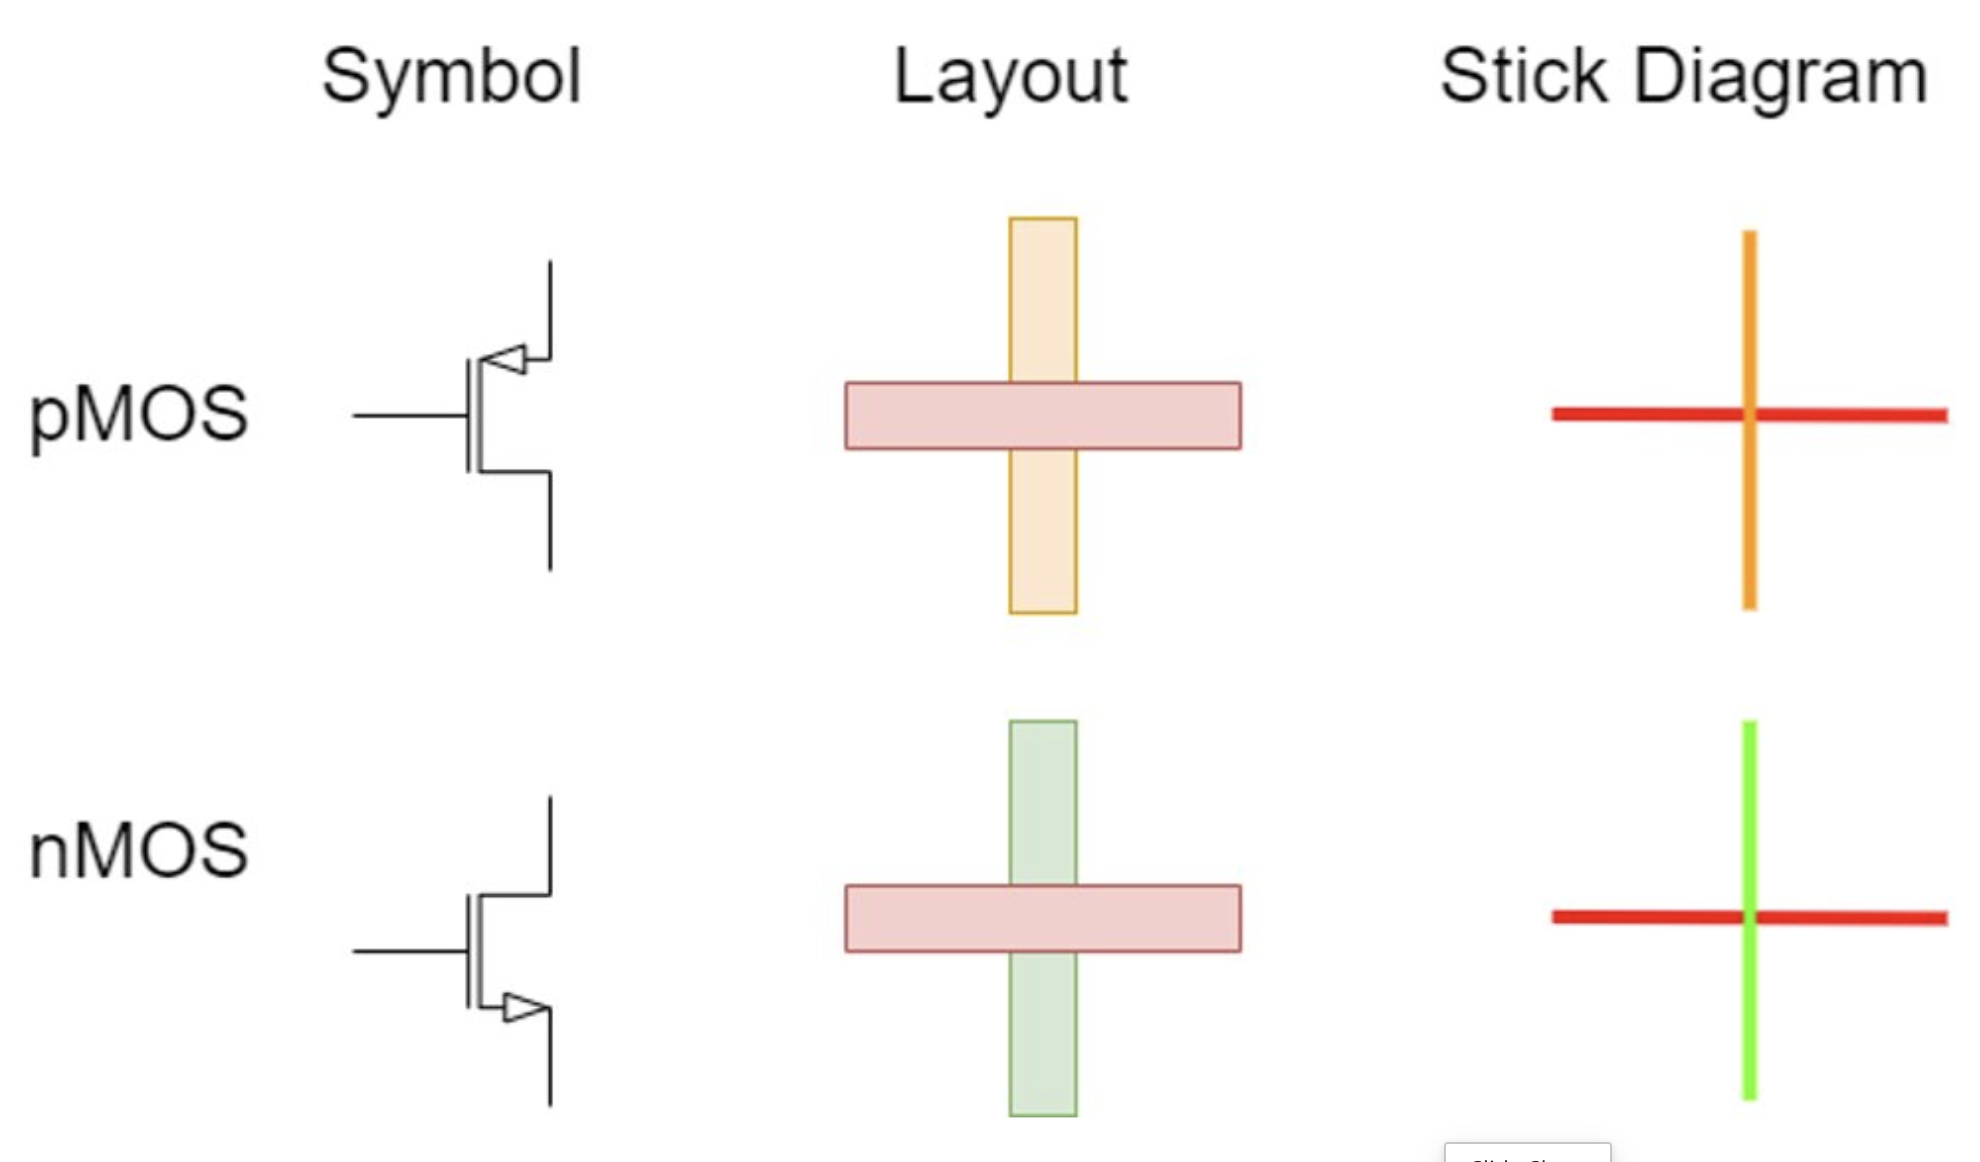
\includegraphics[width=0.5\textwidth]{convenzione-stick-diagram.png}
    \caption{Convenzione di rappresentazione nello Stick-Diagram}
    \label{fig:convensione_stick_diagram}
\end{figure}

\noindent
in cui nel primo caso le barre arancioni verticali rappresentano la zona drogata $p$, mentre le barre verdi verticali rappresentano la zona drogata $n$. La barra orizzontale rossa non è altro che il silicio policristallino.

\newpage
\noindent
\textbf{Esempio 1}: Nel caso dell'invertitore CMOS, per esempio, si ottiene una rappresentazione approssimata del circuito finale, realizzata nella raffigurazione intermedia della figura seguente:

\begin{figure}[H]
    \centering
    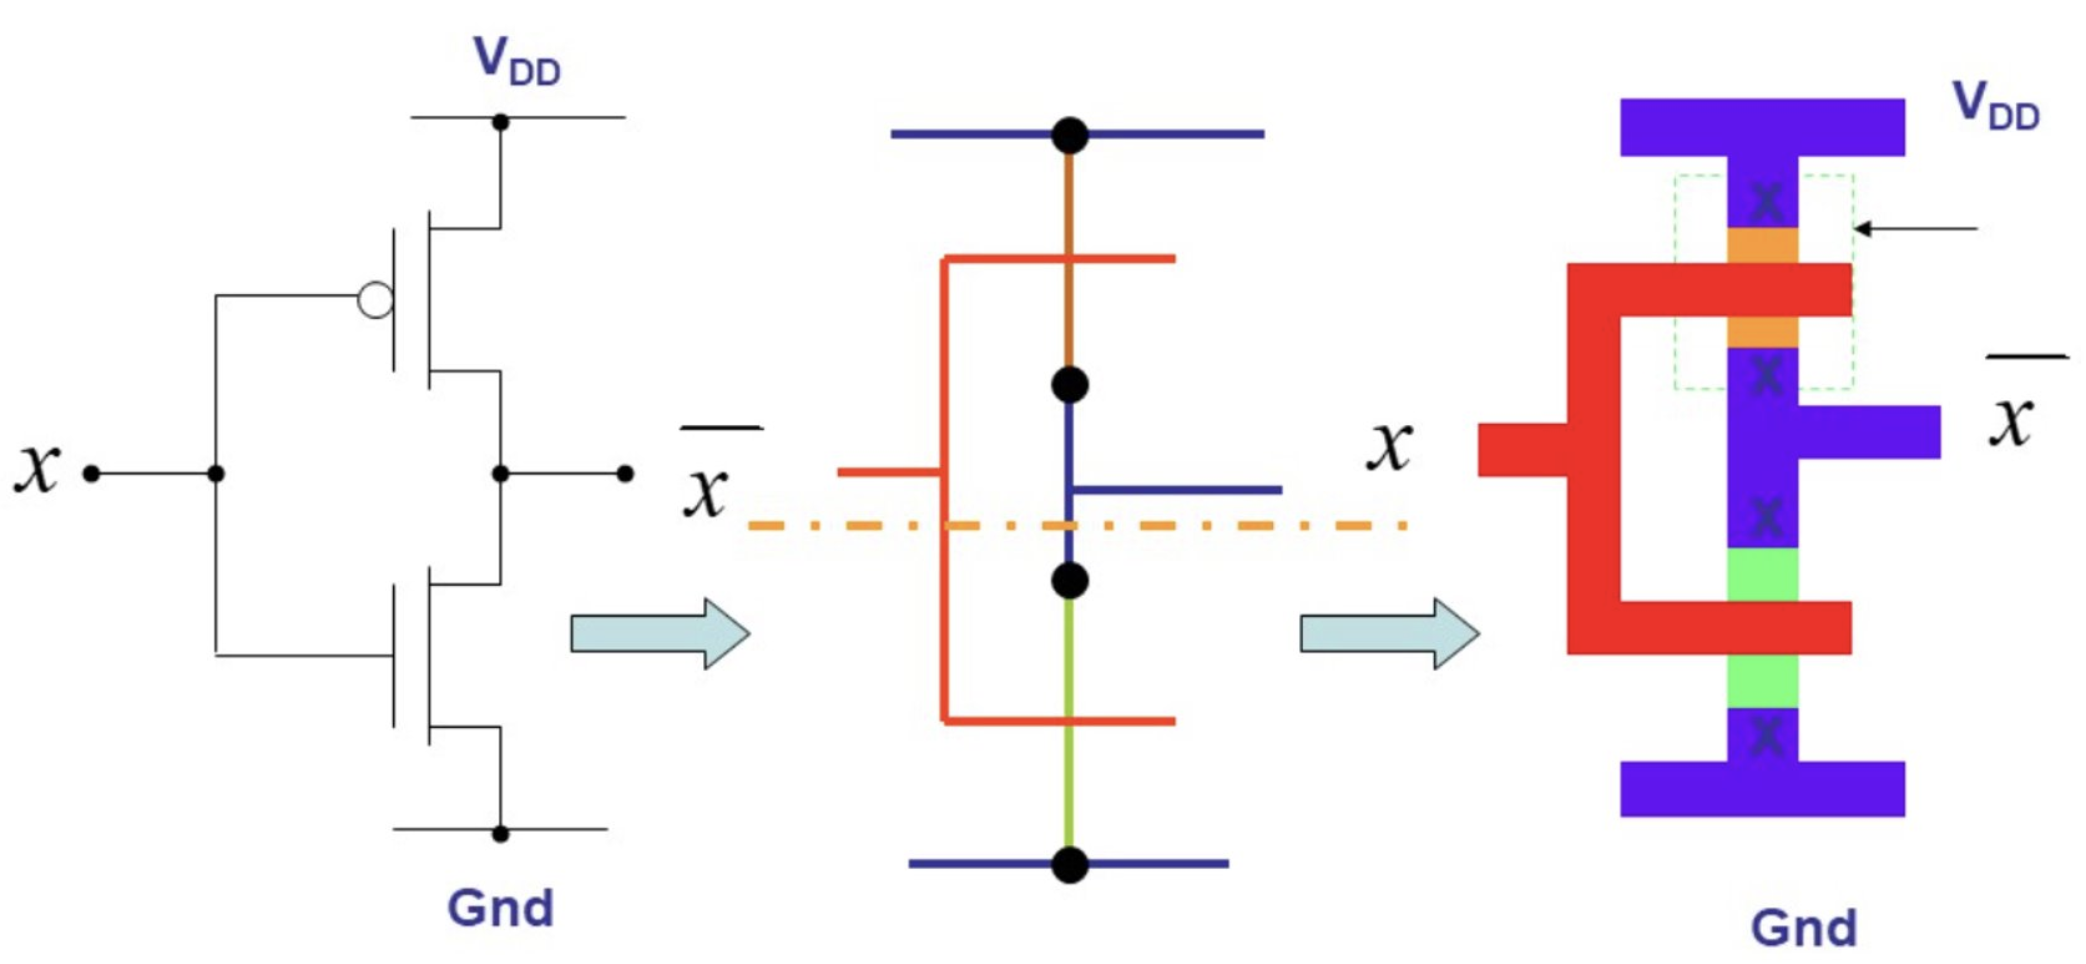
\includegraphics[width=0.6\textwidth]{stick-diagram-esempio-1.png}
    \caption{Invertitore CMOS con lo Stick-Diagram}
    \label{fig:invertitore_cmos_stick_diagram}
\end{figure}

\vspace{1em}
\noindent
Le regole da impiegare nella rappresentazione sono le seguenti:
\begin{itemize}
    \item L'intersezione tra due \quotes{sticks} del medesimo tipo rappresenta un contatto;
    \item L'intersezione tra due \quotes{sticks} di tipo diverso NON rappresenta un contatto;
    \item Per evidenziare un contatto tra elementi diversi si deve usare un VIA (ossia un pallino);
    \item L'intersezione tra il silicio policristallino (rosso) e l'area attiva (drogata $p$, arancione, o drogata $n$, verde) rappresenta un transistor;
    \item L'intersezione tra silicio policristallino e l'area attiva con un VIA non rappresenta un transistor;
    \item I transistor a canale-$n$ e a canale-$p$ devono essere ai lati opposti della linea di demarcazione. I due tipi di transistor devono stare in zone separate del circuito, divisi nettamente per tipologia.
\end{itemize}

\vspace{1em}
\noindent
\textbf{Esempio 2}: La porta NOR viene raffigurata, tramite lo stick diagram, nel modo seguente seguente:

\begin{figure}[H]
    \centering
    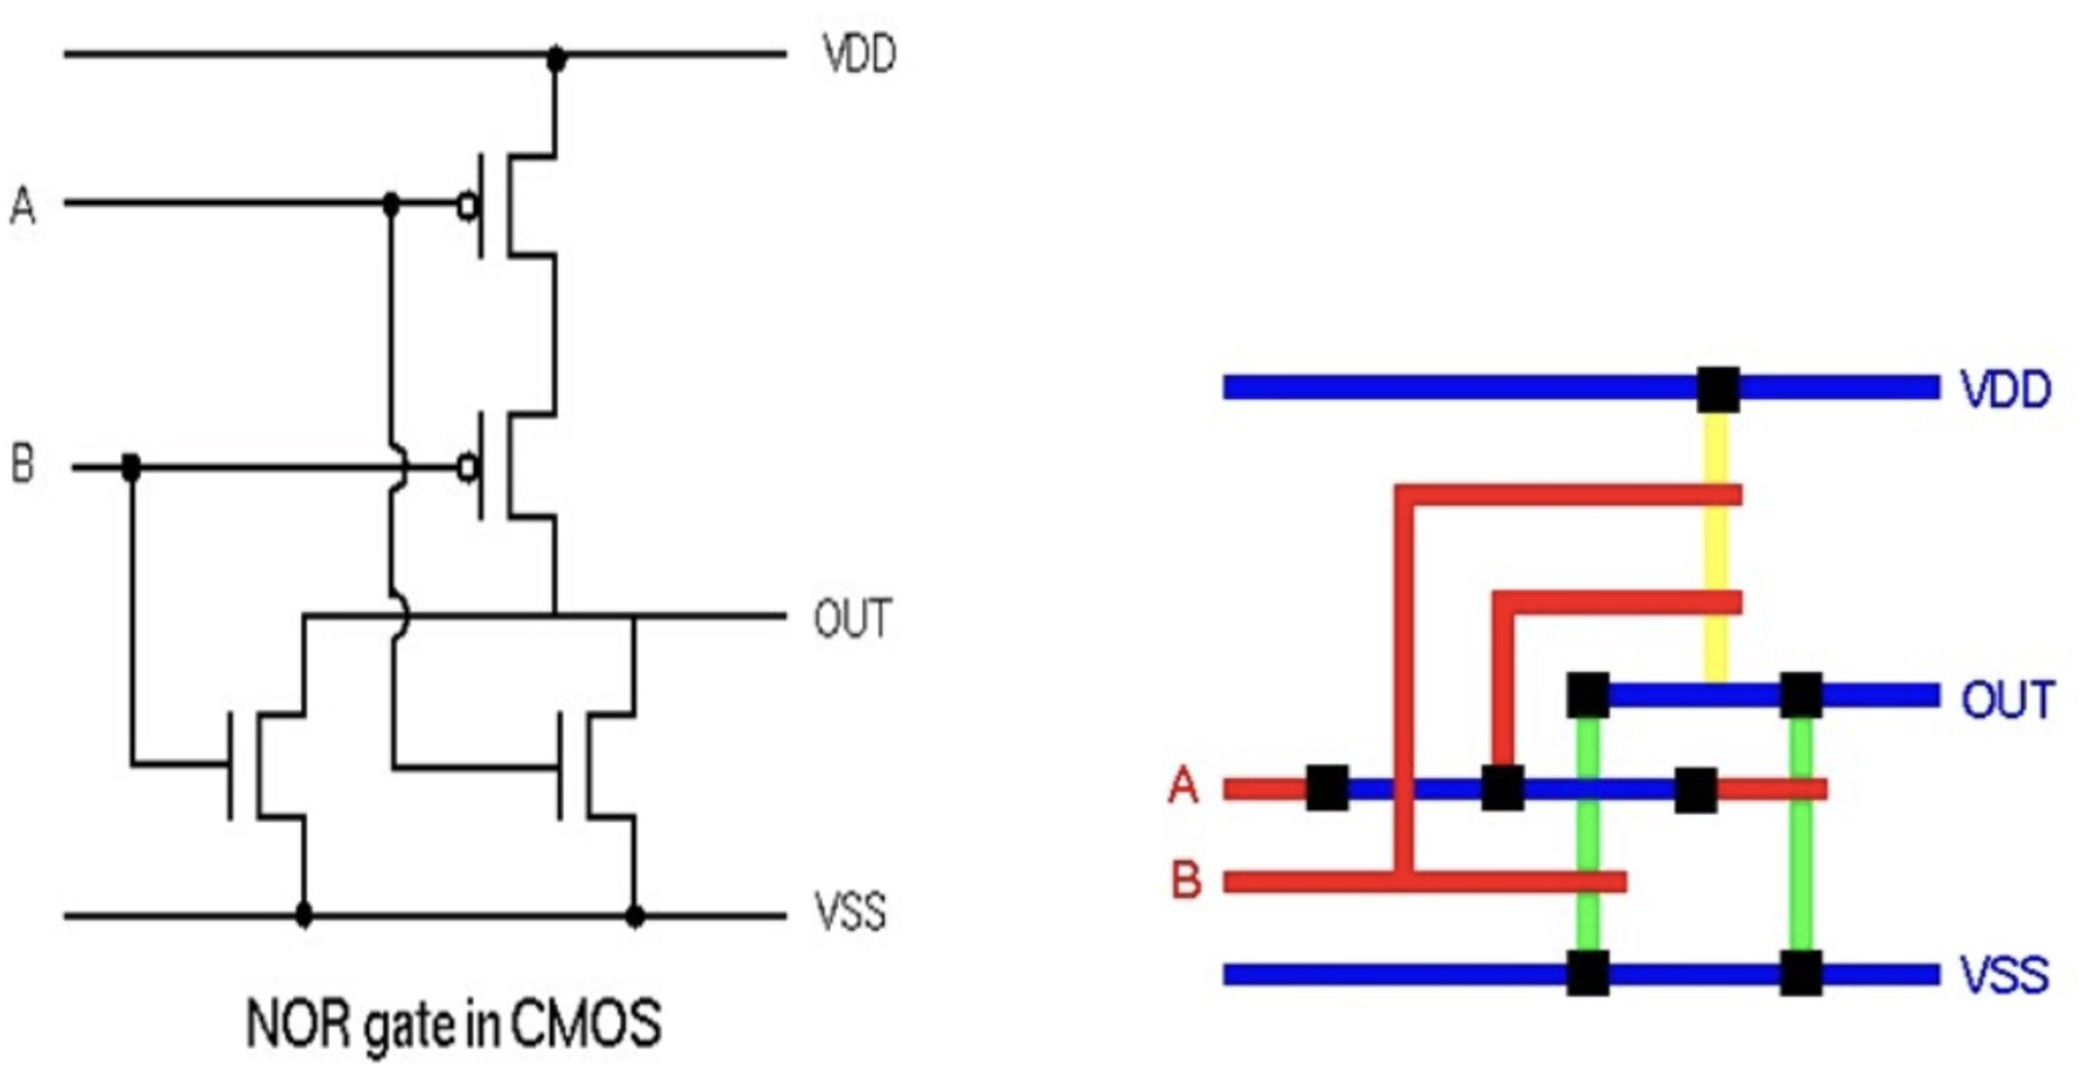
\includegraphics[width=0.6\textwidth]{stick-diagram-esempio-2.png}
    \caption{NOR in CMOS con lo Stick-Diagram}
    \label{fig:nor_cmos_stick_diagram}
\end{figure}

\noindent
in cui bisogna prestare molta attenzione ai contatti e all'intersezione delle linee: nel caso del collegamento orizzontale del segnale $A$, non si poteva creare un'intersezione tra linee rosse, in quanto ciò avrebbe costituito un contatto; similmente, successivamente, non si doveva intersecare la linea rossa con quella verde perché lì si sarebbe venuto a creare un transistor a canale-$n$ non previsto nella progettazione circuitale. Pertanto si sostituisce al collegamento problematico una linea metal.

\vspace{1em}
\noindent
\textbf{Esempio 3}: La porta OAI a $3$ ingressi viene raffigurata, tramite lo stick diagram, nel modo seguente seguente:

\begin{figure}[H]
    \centering
    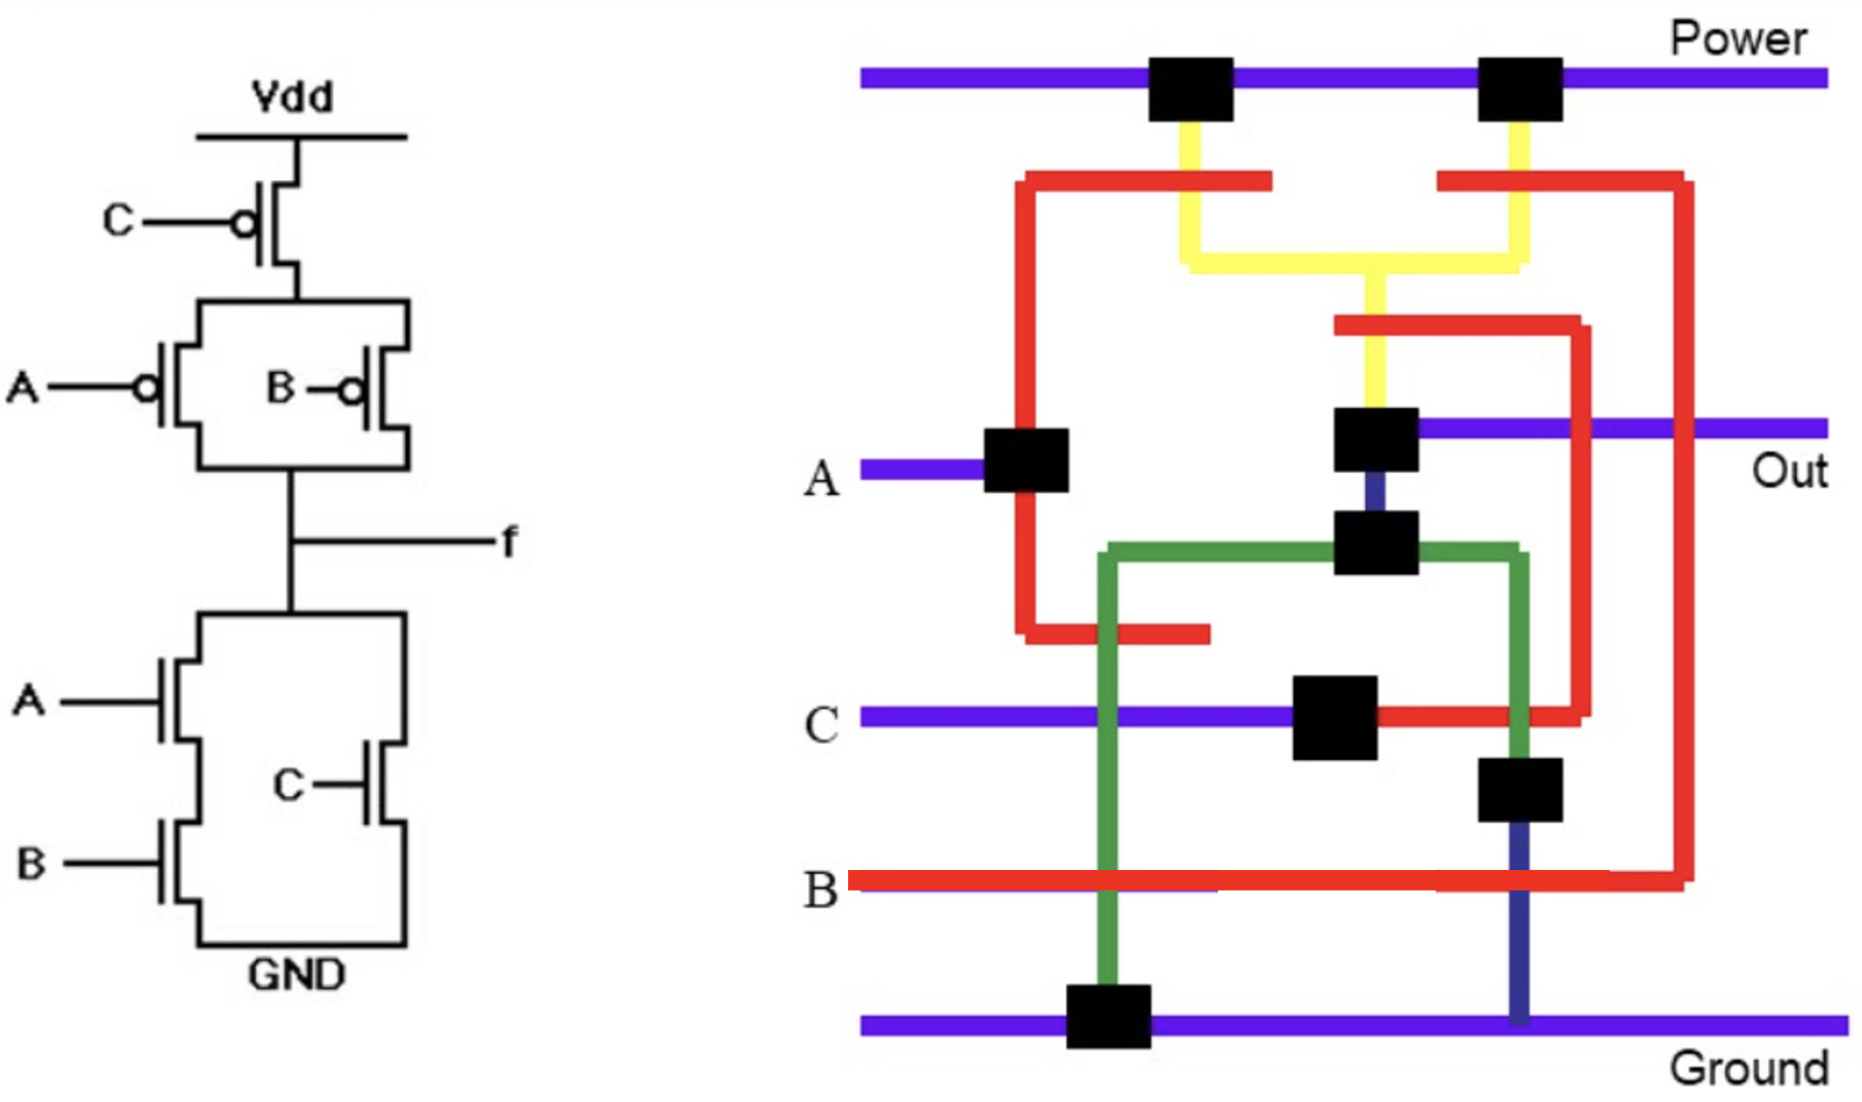
\includegraphics[width=0.6\textwidth]{stick-diagram-esempio-3.png}
    \caption{OAI a $3$ ingressi in CMOS con lo Stick-Diagram}
    \label{fig:oai_3_ingressi_cmos_stick_diagram}
\end{figure}

\newpage
\begin{center} 
    20 Ottobre 2022
\end{center}

\vspace{1em}
\noindent
\subsection{Termini minimi}
I termini minimi sono dei termini che valgono $1$ solo per una certa configurazione degli ingressi. I termini minimi si ottengono come prodotto di tutte le variabili (di cui alcune dirette ed alcune negate). Per esempio, si hanno:
\[\overline{x_1} \cdot x_4 \hspace{1em} \text{e} \hspace{1em} x_3 \cdot \overline{x_2}\]
È importante osservare che
\begin{itemize}
    \item Ogni funzione può essere rappresentata come somma di termini minimi, denominata \textbf{I forma canonica};
    \item Ogni funzione è esprimibile come somma di prodotti;
\end{itemize}

\vspace{1em}
\noindent
\subsection{Termini massimi}
I termini massimi sono dei termini che valgono $0$ solo per una certa configurazione degli ingressi. I termini massimi si ottengono come somma di tutte le variabili (di cui alcune dirette ed alcune negate). Per esempio, si hanno:
\[\overline{x_1} + x_4 \hspace{1em} \text{e} \hspace{1em} x_3 + \overline{x_2}\]
È importante osservare che
\begin{itemize}
    \item Ogni funzione può essere rappresentata come prodotto di termini massimi, denominata \textbf{II forma canonica};
    \item Ogni funzione è esprimibile come prodotto di somme.
\end{itemize}

\vspace{1em}
\noindent
\subsection{Teoremi fondamentali}
Di seguito si espongono alcuni fondamentali teoremi alla base della semplificazione e della comprensione dell'Algebra Booleana.

\vspace{1em}
\noindent
\subsubsection{Principio di dualità}
Tutti i postulati fino ad ora esposti, possono essere accoppiati tra loro e si può ottenere l'uno dall'altro pur di effettuare le seguenti sostituzioni
\begin{itemize}
    \item ogni $1$ deve divenire uno $0$ e viceversa;
    \item ogni prodotto diviene una somma e viceversa.
\end{itemize}
Per esempio si ha che
\begin{align*}
    &(x_1 \cdot x_2) + (x_1 \cdot x_3) = x_1 \cdot (x_2 + x_3)\\
    &(x_1 + x_2) \cdot (x_1 + x_3) = x_1 + (x_2 \cdot x_3)
\end{align*}

\vspace{1em}
\noindent
\subsubsection{Teoremi dell'assorbimento}
I teoremi dell'assorbimento si dividono in:
\begin{enumerate}
    \item Primo teorema dell'assorbimento:
    \[x+xy=x \cdot (1+y)=x\]
    \item Secondo teorema dell'assorbimento:
    \[x+\overline{x} y = x \cdot (1+y)+\overline{x}y = x + xy + \overline{x}y = x + (x + \overline{x}) \cdot y = x+y\]
    \item Terzo teorema dell'assorbimento:
    \[xy+yz+\overline{x}z=xy\overline{x}z\]
\end{enumerate}

\vspace{1em}
\noindent
\subsection{Teorema di De Morgan}
Il teorema di De Morgan stabilisce la seguenti uguaglianze:
\[\overline{x+y}=\overline{x} \cdot \overline{y} \hspace{1em} \text{e} \hspace{1em} \overline{x \cdot y} = \overline{x} + \overline{y}\]
ovvero, generalizzando, si ottiene che
\[\overline{F(x_1,x_2,\dots,+,\cdot)} = F(\overline{x_1},\overline{x_2},\overline{\dots},\cdot,+)\]
Ovvero la negazione di una funzione si ottiene negando le sue variabili e scambiando tra loro gli operatori di somma e prodotto.

\vspace{1em}
\noindent
\textbf{Osservazione}: Tramite il teorema di De Morgan si può verificare l'equivalenza fra le forme canoniche:
\[y=\sum y_i \cdot m_i = \overline{\overline{y}} = \overline{\sum \overline{y_i} \cdot m_i} = \prod (y_i + \overline{m_i}) = \prod (y_i + M_i)\]
si può verificare che l'insieme completo degli operatori necessario e sufficiente per rappresentare qualsiasi funzione logica non è AND, OR, NOT ma solamente AND e NOT oppure OR e NOT
\begin{align*}
    &x+y=\overline{\overline{x+y}}=\overline{\overline{x} \cdot \overline{y}}
    &x \cdot y=\overline{\overline{x \cdot y}}=\overline{\overline{x} + \overline{y}}
\end{align*}

\vspace{1em}
\noindent
\subsection{Teorema di Shannon}
Il teorema di Shannon afferma che è sempre possibile esprimere una funzione booleana come segue
\[f(x_1,x_2,\dots,x_n)=x_1 \cdot f(1,x_2,\dots,x_n) + \overline{x_1} \cdot f(0,x_2,\dots,x_n)\]
Ciò è vero in quanto
\begin{itemize}
    \item se $x_1=1$ allora
    \[f(1,x_2,\dots,x_n)=1 \cdot f(1,x_2,\dots,x_n) + 0 \cdot f(0,x_2,\dots,x_n)\]
    \item se $x_1=0$ allora
    \[f(0,x_2,\dots,x_n)=0 \cdot f(1,x_2,\dots,x_n) + 1 \cdot f(0,x_2,\dots,x_n)\]
\end{itemize}

\vspace{1em}
\noindent
\subsection{Funzioni universali}
Le funzioni NAND e NOR sono anche dette \textbf{funzioni universali}, in quanto tramite esse si può realizzare qualunque funzione logica:
\begin{align*}
    &\overline{x}=x \vert x & & \overline{x} = x \downarrow x\\
    &x \cdot y = \overline{x \vert y} & & x \cdot y = \overline{\overline{x}+\overline{y}} = \overline{x} \downarrow \overline{y}\\
    &x+y=\overline{\overline{x} \cdot \overline{y}}=\overline{x} \vert \overline{y} & & x+y = \overline{x \downarrow y}
\end{align*}

\vspace{1em}
\noindent
\subsection{Semplificazione di funzioni}
Di seguito si espongono alcuni fondamentali concetti impiegabili nella semplificazione di funzioni booleane:
\begin{itemize}
    \item \textbf{Letterale}: è la coppia variabile-valore; ad ogni variabile sono associati $a$ letterali ($a$ ed $\overline{a}$);
    \item \textbf{Implicante} di una funzione 
    \[f(x_1,\dots,x_n)\]
    è il prodotto di letterali 
    \[P=x_i \cdot \dots \cdot x_k\]
    in forma diretta o negata, tale per cui se $P=1$ anche $f=1$;
    \item \textbf{Termine minimo}: è implicante ove compaiono tutte le variabili, ovvero è un punto nello spazio booleano della funzione dove la funzione vale $1$;
    \item \textbf{On set} di una funzione: è l'insieme dei suoi termini minimi;
    \item \textbf{Termine massimo}: è un punto nello spazio booleano della funzione dove la funzione vale $0$;
    \item \textbf{Off set} della funzione: è l'insieme di tutti i punti dello spazio booleano della funzione che non sono termini minimi;
    \item \textbf{Implicante}: è un sotto-cubo di soli $1$ nello spazio booleano della funzione;
    \item \textbf{Implicante primo}: è un implicante che è contenuto in altri implicanti;
    \item \textbf{Implicante essenziale}: è un implicante che contiene almeno un $1$ non incluso in altri implicanti primi;
    \item \textbf{Copertura} di una funzione: è l'insieme di implicanti che coprono tutti i termini minimi.
\end{itemize}

\vspace{1em}
\noindent
\textbf{Osservazione}: Ovviamene, due funzioni sono equivalenti se hanno la stessa tavola di verità e per semplificare una funzione possono essere impiegate differenti strategie:
\begin{itemize}
    \item attraverso le relazioni fondamentali e i teoremi dell'Algebra Booleana;
    \item individuando termini implicanti
    \item tramite le \textbf{Mappe di Karnaugh} (forma minima a 2 livelli, ma prevalentemente somma di prodotti), ovvero delle tabelle toroidali che rappresentano in più dimensioni la tabella di verità della funzione;
    \item attraverso il \textbf{Metodo tabellare di Quine-McCluskey} (forma minima a 2 livelli), basato sull'applicazione sistematica del teorema di Shannon
    \[f \cdot x + f \cdot \overline{x} = f\]
\end{itemize}
Ma naturalmente vi possono essere forme più\quotes{economiche} (a più livelli) per realizzare una funzione che questi metodi non evidenziano.

\vspace{1em}
\noindent
\subsection{Condizioni non specificate (Don't care)}
In una realtà circuitale, vi possono essere condizioni di ingresso che non si verificano: ad esempio, se gli ingressi dipendono a loro volta da una rete logica.\\
La presenza di tali condizioni può essere ben impiegata per generare ulteriori semplificazioni: infatti, una condizione non specificata (\textit{Don't care}) si può considerare diretta o negata, in funzione di quale fornisce la miglior semplificazione.

\vspace{1em}
\noindent
\subsection{Simmetria di funzioni}
Le funzioni simmetriche possono essere implementate facilmente, ma esclusivamente, con tecniche particolari; infatti, non funzionano i normali metodi di semplificazione.\\
Nell'ambito della simmetria di funzioni si distinguono funzioni
\begin{itemize}
    \item \textbf{totalmente simmetriche}, in cui un qualsiasi scambio tra le variabili lascia immutato il risultato; l'intercambiabilità può essere anche tra variabili dirette e negate (anche se meno evidente);
    \item \textbf{parzialmente simmetriche}, in cui la proprietà di cui sopra è limitata ad un sottoinsieme di variabili;
    \item \textbf{simmetriche indipendenti}, in cui la simmetria esiste solo per un sottoinsieme della funzione
\end{itemize}
In tutti i casi esposti in precedenza, le variabili interessate possono essere dirette, negate o miste.

\newpage
\begin{center} 
    21 Ottobre 2022
\end{center}
Le funzioni booleane si dicono simmetriche se qualsiasi scambio tra le variabili porta al medesimo risultato.

\vspace{1em}
\noindent
\subsubsection{Primo teorema di simmetria}
Il primo teorema di simmetria delle funzioni booleane afferma che:

% Tabella per le definizione di concetti, etc...
\vspace{1em}
\rowcolors{1}{black!5}{black!5}
\setlength{\tabcolsep}{14pt}
\renewcommand{\arraystretch}{2}
\noindent
\begin{tabularx}{\textwidth}{@{}|P|@{}}
    \hline
    {\textbf{PRIMO TEOREMA DI SIMMETRIA}}\\
    \parbox{\linewidth}{ll valore della funzione dipende da quante variabili valgono $1$ e non da quali.\vspace{3mm}}\\
    \hline
\end{tabularx}

\vspace{1em}
\noindent
Condizione necessaria e sufficiente affinché una funzione di commutazione di $n$ variabili sia simmetrica è che essa possa essere individuata da un insieme di interi $\{a_k\}$ con $0 \leq a \leq n$, in modo che se esattamente $a_m$, con $m = 1,2,\dots, k$ delle variabili valgono $1$, la funzione valga $1$, mentre valga $0$ negli altri casi.\\
Ciò, pertanto, significa che
\begin{itemize}
    \item essendo una condizione sufficiente, se esiste l'insieme, allora la funzione è simmetrica.\\
    Si consideri una funzione che vale $1$ se e solo se $N$, con $N=a_m$, variabili sono poste a $1$; allora, scambiando $2$ variabili qualunque si ottiene lo stesso risultato, ovvero la funzione è simmetrica;

    \item essendo una condizione necessaria, se non esiste l'insieme, la funzione non è simmetrica.\\
    Si consideri una funzione in cui non è definibile l'insieme di cui sopra. Esisterà, pertanto, almeno un caso in cui la funzione con certe variabili poste a $1$ vale $1$, mentre, pur mantenendo lo stesso numero di variabili poste a $1$, ma organizzate in altro modo, vale $0$. Poiché a questa condizione si può pervenire tramite scambio tra variabili, ne consegue che la funzione NON sarà simmetrica. Per esempio
    \[F(1,1,0,0, 1,0,1) = 1 \hspace{1em} \text{e} \hspace{1em} F(1,1,1,0,1,0,0) = 0\]
\end{itemize}
Pertanto se una funzione è simmetrica, il suo valore dipende esclusivamente dal peso della parola in ingresso; se il peso in ingresso, per esempio, sta all'interno dell'insieme $\{0,2,3\}$, allora l'uscita è $1$, sarà $0$ altrimenti.\\
Se, pertanto, la funzione è simmetrica, allora è anche più facilmente realizzabile, in quanto è sufficiente creare un circuito per il calcolo del peso della parola (ossia un sommatore bit a bit della parola) e, successivamente, tramite una logica, definire il valore della funzione in uscita:

\begin{figure}[H]
    \centering
    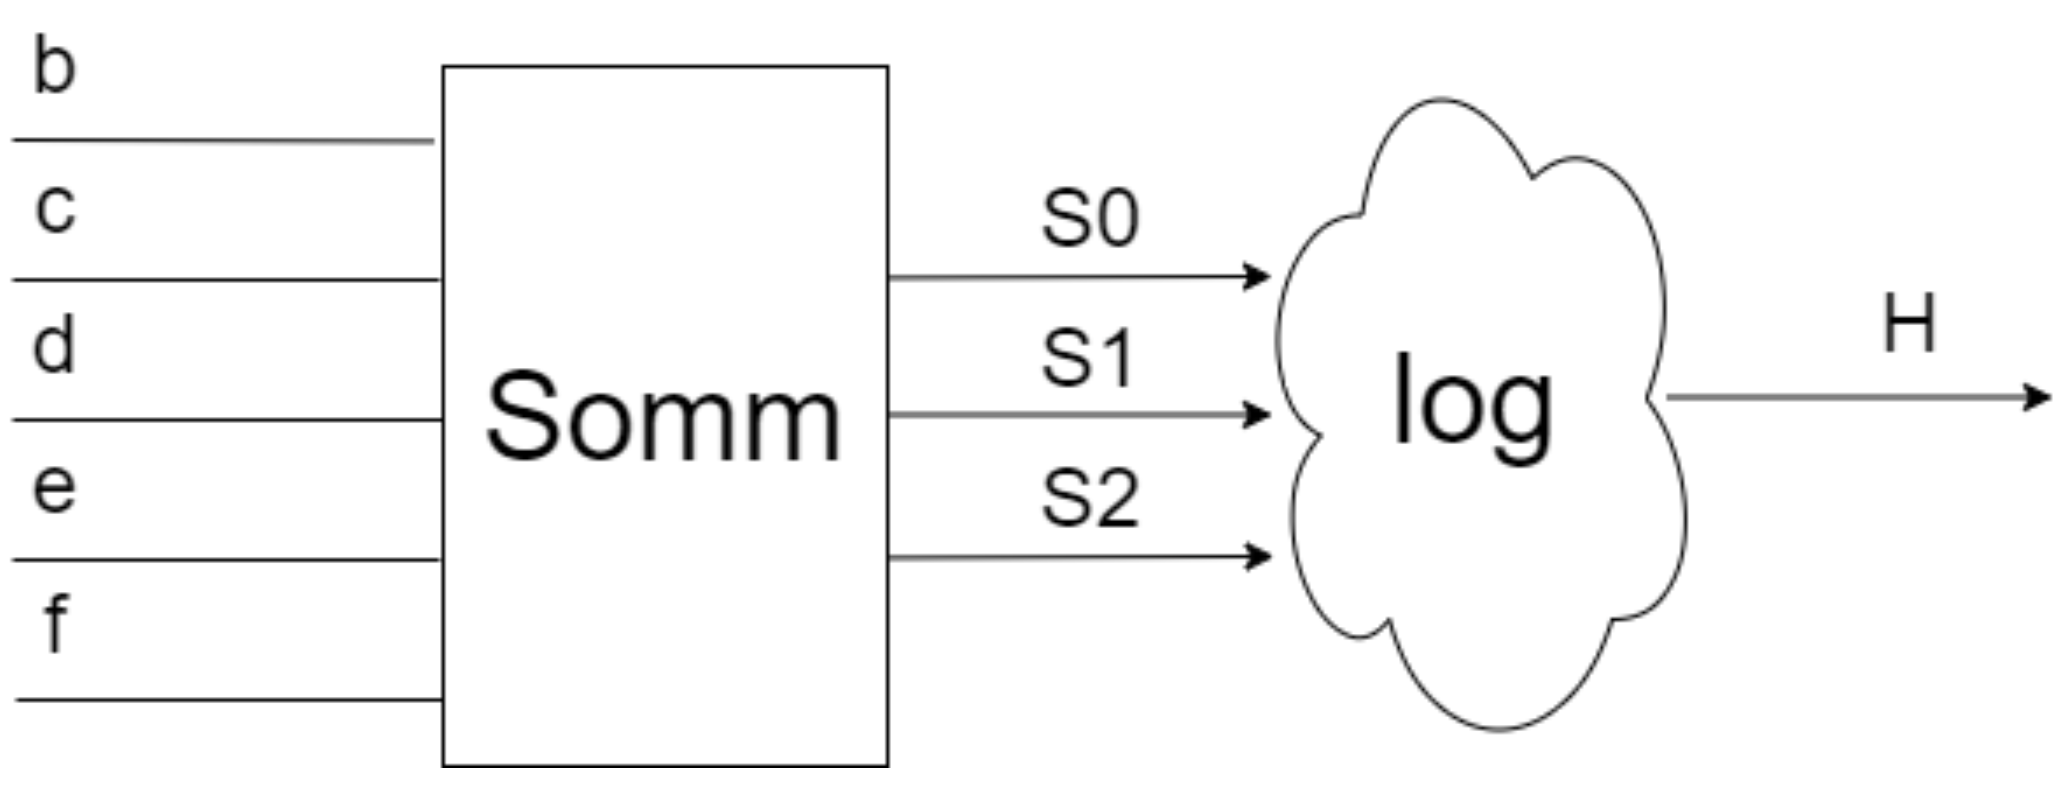
\includegraphics[width=0.7\textwidth]{logica-realizzazione-funzione-simmetrica.png}
    \caption{Logica di realizzazione di una funzione simmetrica}
    \label{fig:logica_realizzazione_funzione_simmetrica}
\end{figure}

\noindent
Poiché il numero di ingressi è pari a $5$ nell'esempio preso in esame, il sommatore restituirà sulle linee $[S2 \dots S0]$ un valore compreso tra $0$ e $5$, ovvero un numero binario su $3$ bit compreso tra $000$ e $101$.\\
La realizzazione del sommatore può seguire, quindi, il procedimento a cascata che vede l'utilizzo di 2 Full-Adder per sommare i $5$ bit in ingresso ed un ulteriore Half-Adder per sommare i riporti da questi generati:

\begin{figure}[H]
    \centering
    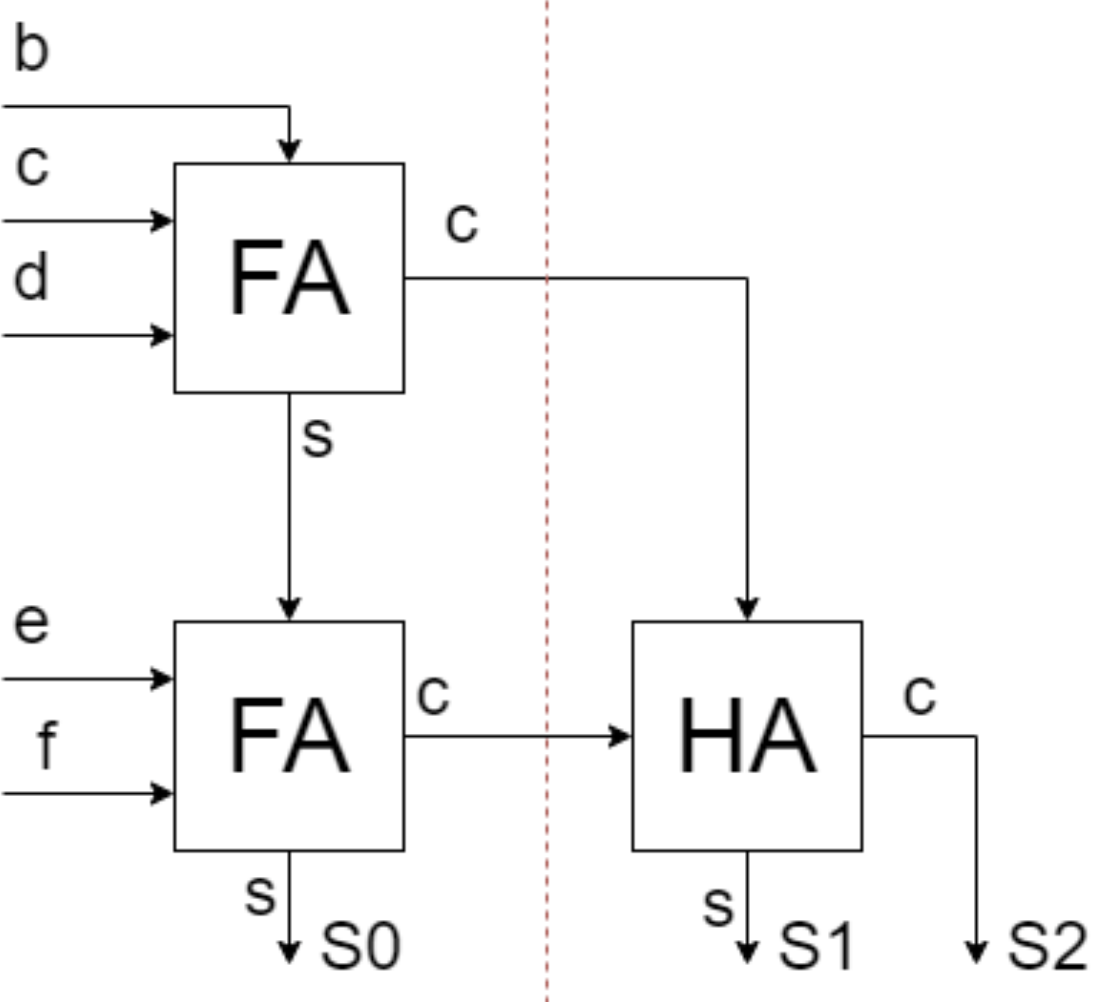
\includegraphics[width=0.6\textwidth]{sommatore-calcolo-peso-parola.png}
    \caption{Sommatore per il calcolo del peso della parola}
    \label{fig:sommatore_calcolo_peso_parola}
\end{figure}

\noindent
in cui il bit più significativo è $S2$, mentre quello meno significativo è $S1$: pertanto il risultato deve essere letto come $S2 S1 S0$. La logica di realizzazione finale può essere facilmente determinata; per esempio, se si vuole fare in modo che la funzione valga $1$ solamente quando il peso è $3$, $4$ oppure $5$ si ottiene

\vspace{1em}
\noindent
\begin{table}[H]
\rowcolors{1}{white}{white}
\setlength{\tabcolsep}{4pt}
\renewcommand{\arraystretch}{1.2}
\centering
\begin{tabular}{|c|c|c|c|c|}
    \hline
    peso & $S2$ & $S1$ & $S0$ & $R1$\\
    \hline
    $0$ & $0$ & $0$ & $0$ & $0$\\
    $1$ & $0$ & $0$ & $1$ & $0$\\
    $2$ & $0$ & $1$ & $0$ & $0$\\
    $3$ & $0$ & $1$ & $1$ & $1$\\
    $4$ & $1$ & $0$ & $0$ & $1$\\
    $5$ & $1$ & $0$ & $1$ & $1$\\
    $6$ & $1$ & $1$ & $0$ & $-$\\
    $7$ & $1$ & $1$ & $1$ & $-$\\
    \hline
\end{tabular}
\end{table}

\vspace{1em}
\noindent
Si noti in particolare la presenza di valori non definiti per le combinazioni $110$ e $111$ che NON potranno mai verificarsi all'ingresso.\\
I termini minimi possono essere organizzati per maggior chiarezza in una mappa di Karnaugh

\vspace{1em}
\noindent
\begin{table}[H]
\rowcolors{1}{white}{white}
\setlength{\tabcolsep}{4pt}
\renewcommand{\arraystretch}{1.2}
\centering
\begin{tabular}{|c|c|c|c|c|}
    \hline
    $S2/S1$ & $ $ & $ $ & $ $ & $ $\\
    $S0$ & $00$ & $01$ & $11$ & $10$\\
    \hline
    $0$ & $0$ & $0$ & $-$ & $1$\\
    \hline
    $1$ & $0$ & $1$ & $-$ & $1$\\
    \hline
\end{tabular}
\end{table}

\vspace{1em}
\noindent
In cui appare evidente come la semplificazione sia
\[H  = S2 + S0S1\]
che in forma circuitale diviene

\begin{figure}[H]
    \centering
    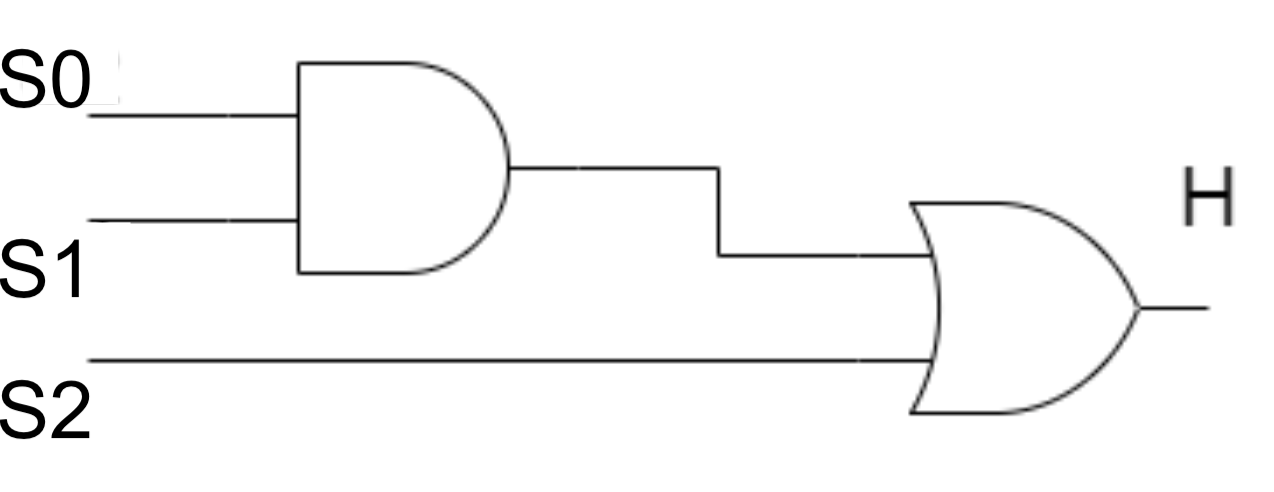
\includegraphics[width=0.6\textwidth]{realizzazione-logica.png}
    \caption{Logica per la funzione}
    \label{fig:logia_funzione}
\end{figure}

\vspace{1em}
\noindent
\subsubsection{Conseguenza del primo teorema}
Come naturale conseguenza del primo teorema, una funzione simmetrica può essere rappresentata tramite l'insieme caratteristico e le variabili di simmetria:
\[S^n_{\{a_k\}}(x_1^{j_1}, x_2^{j_2}, \dots, x_n^{j_n})\]
in cui, ovviamente, $n$ è il numero di variabili rispetto al quale la funzione è simmetrica, mentre i livelli di simmetria sono definiti dall'insieme $\{a_k\}$, contente, quindi, i pesi rispetto ai quali la funzione $f$ deve rispondere affermativamente. Ovviamente, le variabili $x_1^{j_1}, x_2^{j_2}, \dots, x_n^{j_n}$ possono essere tanto dirette quanto negate.

\vspace{1em}
\noindent
\subsubsection{Secondo teorema di simmetria}
Il secondo teorema di simmetria delle funzioni booleane afferma che:

% Tabella per le definizione di concetti, etc...
\vspace{1em}
\rowcolors{1}{black!5}{black!5}
\setlength{\tabcolsep}{14pt}
\renewcommand{\arraystretch}{2}
\noindent
\begin{tabularx}{\textwidth}{@{}|P|@{}}
    \hline
    {\textbf{SECONDO TEOREMA DI SIMMETRIA}}\\
    \parbox{\linewidth}{La somma di più funzioni simmetriche nelle stesse variabili è ancora una funzione simmetrica avente come livelli di simmetria tutti i livelli delle funzioni simmetriche di partenza (ossia l'unione dei livelli di simmetria).\vspace{3mm}}\\
    \hline
\end{tabularx}

\vspace{1em}
\noindent
\textbf{Dimostrazione}: Essendo le funzioni di partenza simmetriche, uno scambio tra variabili non altera il risultato dei singoli termini e pertanto nemmeno della somma.\\
Ogni funzione, inoltre, vale $1$ se e solo se $n$ variabili sono
affermate (con $n = a_m$, ossia il livello proprio di quella funzione). La funzione somma, quindi, sarà uguale a $1$ se almeno una delle funzioni componenti sarà $1$.

\vspace{1em}
\noindent
\subsubsection{Terzo teorema di simmetria}
Il terzo teorema di simmetria delle funzioni booleane afferma che:

% Tabella per le definizione di concetti, etc...
\vspace{1em}
\rowcolors{1}{black!5}{black!5}
\setlength{\tabcolsep}{14pt}
\renewcommand{\arraystretch}{2}
\noindent
\begin{tabularx}{\textwidth}{@{}|P|@{}}
    \hline
    {\textbf{TERZO TEOREMA DI SIMMETRIA}}\\
    \parbox{\linewidth}{ll prodotto di piu' funzioni simmetriche delle stesse variabili e' ancora una funzione simmetrica avente come livelli di simmetria tutti i livelli comuni alle funzioni simmetriche di partenza (ossia l'intersezione dei livelli di simmetria).\vspace{3mm}}\\
    \hline
\end{tabularx}

\vspace{1em}
\noindent
\textbf{Dimostrazione}: Essendo le funzioni di partenza simmetriche, uno scambio tra variabili non altera il risultato dei singoli termini e pertanto nemmeno del prodotto.\\
Ogni funzione vale $1$ se e solo se $n$ variabli sono
affermate (con $n = a_m$, ossia il livello proprio di quella funzione).\\
La funzione prodotto sarà uguale a $1$ se tutte le funzioni componenti valgono $1$.

\vspace{1em}
\noindent
\subsubsection{Quarto teorema di simmetria}
Il quarto teorema di simmetria delle funzioni booleane afferma che:

% Tabella per le definizione di concetti, etc...
\vspace{1em}
\rowcolors{1}{black!5}{black!5}
\setlength{\tabcolsep}{14pt}
\renewcommand{\arraystretch}{2}
\noindent
\begin{tabularx}{\textwidth}{@{}|P|@{}}
    \hline
    {\textbf{QUARTO TEOREMA DI SIMMETRIA}}\\
    \parbox{\linewidth}{La negazione di una funzione simmetrica di $n$ variabili e di livelli $\{a_k\}$ è ancora una funzione simmetrica di $n$ variabili i cui livelli di simmetria $\{a_j\}$ sono il complemento dei livelli $\{a_k\}$.    
    \vspace{3mm}}\\
    \hline
\end{tabularx}

\vspace{1em}
\noindent
\textbf{Dimostrazione}: Essendo la funzione di partenza simmetriche, uno scambio tra variabili non altera il risultato e pertanto nemmeno il risultato dell'inversione.\\
Poiché per definizione la funzione originale vale $1$ se e solo se $n$ variabili sono affermate (con $n = am$ appartenente ad $\{a_k\}$) la funzione negata sarà uguale a $1$ se e solo se $n \neq a_m$ appartenente ad $\{a_k\}$, ovvero se $n=a_m$ appartenente ad $\{a_j\}$.

\vspace{1em}
\noindent
\subsubsection{Quinto teorema di simmetria}
Il quinto teorema di simmetria delle funzioni booleane afferma che:

% Tabella per le definizione di concetti, etc...
\vspace{1em}
\rowcolors{1}{black!5}{black!5}
\setlength{\tabcolsep}{14pt}
\renewcommand{\arraystretch}{2}
\noindent
\begin{tabularx}{\textwidth}{@{}|P|@{}}
    \hline
    {\textbf{QUINTO TEOREMA DI SIMMETRIA}}\\
    \parbox{\linewidth}{Negando le variabili di una funzione simmetrica si ottiene ancora una funzione simmetrica i cui livelli di simmetria sono il complemento a $N$ dei livelli di simmetria della funzione originale (sono tanti
    livelli quanti quelli della funzione originale).
    \vspace{3mm}}\\
    \hline
\end{tabularx}

\vspace{1em}
\noindent
\textbf{Dimostrazione}: Essendo la funzione di partenza simmetrica, uno scambio tra variabili non altera il risultato dei singoli termini e, pertanto, se si opera una negazione di tutte le variabili la proprietà non cambia.\\
Poiché per definizione la funzione originale vale $1$ se e solo se $n$ variabili sono affermate (con $n = am$ appartenente ad $\{a_k\}$), negando tutte le variabili l'uscita sarà uguale a $1$ se e solo se $n$ variabili saranno uguali a $0$ (con $n = am$ appartenente ad $\{a_k\}$, ovvero se le variabili affermate sono
$N-n$).

\vspace{1em}
\noindent
\subsubsection{Conseguenze del quinto teorema}
Ogni funzione simmetrica possiede almeno due centri di simmetria: il primo rispetto certe variabili ed un altro rispetto alle
variabili negate. Pertanto
\[S^3_1(\overline{x},\overline{y},\overline{z}) = S^3_2(x,y,z)\]
Vi possono essere. peraltro, molti centri di simmetria, dati dalle combinazioni dei livelli di simmetria e delle variabili dirette e negate.\\
I centri di simmetria vengono enumerati in base al relativo termine minimo (sono ben visibili nelle mappe di Karnaugh): pertanto $S^3_2(x,\overline{y},z)$ presenta come centro di simmetria $101$.





\newpage
\begin{center}
    27 Ottobre 2022
\end{center}
Se una funzione $f$ di partenza viene scomposta tramite il teorema di Shannon in due funzioni $f_1$ e $f_2$ tale che
\[f=x \cdot f_1 + \overline{x} \cdot f_2\]
e si verifica che le funzioni $f_1$ e $f_2$ sono simmetriche nelle medesime variabili, allora la funzione $f$ di partenza si dice parzialmente simmetrica e possono essere rappresentate tramite un unico sommatore e un circuito combinatorio che riorganizzi le uscite.\\
Potrebbe accadere che le due sotto-funzioni di partenza risultino essere simmetriche in variabili differenti, allora la funzione si dice separatamente simmetrica.

\vspace{1em}
\noindent
\subsection{Funzioni decomponibili}
Una funzione si dice decomponibile quando si riesce a riconoscere che essa può essere scomposta in più sotto-funzioni.\\
Tale approccio segue il \textbf{binomio area-tempo}: migliorando alcuni aspetti della funzione se ne peggiorano degli altri. Infatti, riducendo al minimo possibile la complessità della funzione e del numero di componenti circuitali richiesti per la realizzazione della stessa, aumento il numero di livelli del circuito, con più porte in cascata e un aumento della latenza.

\vspace{1em}
\noindent
\textbf{Osservazione}: Per riconoscere se una funzione può essere decomposta o meno, si impiega il teorema di Shannon. In particolare, si supponga che la funzione $f$ in $4$ variabili che può essere scomposta due volte con Shannon, come mostrato di seguito
\[f(a,b,c,d)=ab \cdot g_1(c,d)+a\overline{b} \cdot g_2(c,d)+\overline{a}b \cdot g_3(c,d)+\overline{a}\overline{b} \cdot g_4(c,d)\]
Ma se si osserva che ciascuna di ogni funzione può essere espressa in funzione di un'unica altra funzione, come, per esempio
\[g_1=g_1\hspace{1em}\text{e}\hspace{1em}g_2=\overline{g_1}\hspace{1em}\text{e}\hspace{1em}g_3=0\hspace{1em}\text{e}\hspace{1em}g_4=1\]
si può realizzare un selettore che a seconda della configurazione di $a$ e $b$ selezioni l'uscita richiesta.

\vspace{1em}
\noindent
\begin{table}[H]
    \rowcolors{1}{white}{white}
\setlength{\tabcolsep}{4pt}
\renewcommand{\arraystretch}{1.2}
\centering
\begin{tabular}{|c|c|c|c|c|}
    \hline
    $ab-cd$ & 00 & 01 & 11 & 10\\
    \hline
    00 & 1  & 0 & 1 & 1\\ 
    \hline
    01 & 0 & 1 & 0 & 1\\ 
    \hline
    11 & 0 & 0 & 0 & 0\\
    \hline
    10 & 1 & 1 & 1 & 1\\
    \hline
\end{tabular}
\end{table}

\vspace{1em}
\noindent
Allora è possibile osservare come la prima riga si possa esprimere in funzione di $cd$, ottenendo $\alpha$, la seconda è $\overline{\alpha}$, la terza riga è $0$, la quarta è $1$.\\
Se la scomposizione della funzione tramite il teorema di Shannon vale sempre, la decomposizione non è sempre realizzabile. Con Shannon, infatti, si è scomposta una funzione a $4$ variabili, per un totale di $16$ combinazione-celle, in $4$ funzioni da $4$ combinazioni-celle, per cui non si è guadagno niente.\\
Ma per capire se una funzione è decomponibile bisogna realizzare tutte le possibile mappe, organizzate con ogni combinazione delle $4$ variabili a disposizione, ponendo, quindi, come riga-colonna $ab-cd$, $ac-bd$, $ad-bc$, $bc-ad$, $bd-ac$ e $cd-ab$, ma anche quando vi è una sola variabile in colonna.

\vspace{1em}
\noindent
\subsubsection{Mappe di decomposizione}
Per decretare se una funzione è decomponibile, si impiegano le cosiddette \textbf{mappe di decomposizione}. A titolo esemplificativo, si consideri la funzione seguente
\[G=ab\overline{c}+ab\overline{d}+\overline{a}bd\]
Allora si considerino i termini di cui è composta, e si determinino i termini minimi da essi generati
\begin{align*}
    &ab\overline{c} &\rightarrow&&110- &&\rightarrow&&\text{termini minimi generati: } 12,13\\
    &ab\overline{d} &\rightarrow&&11-0 &&\rightarrow&&\text{termini minim generati: } 12,14\\
    &\overline{a}bd &\rightarrow&&01-1 &&\rightarrow&&\text{termini minimi generati: } 5,7
\end{align*}
E una volta fatto ciò si considerano le mappe di decomposizione e si evidenziano i termini appena individuati, appartenenti all'insieme
\[\mathcal{Z}=\{5,7,12,13,14\}\]
Se si riesce a identificare una possibile decomposizione, per cui le righe di ogni mappa possono essere espresse in funzione di una funzione $\alpha$ e delle sue possibili varianti, $\overline{\alpha}$, $0$ e $1$, allora si procede con la relativa decomposizione.\\
Nel caso considerato della funzione $G$, decomponendo rispetto alla variabile $b$, si osserva che

\vspace{1em}
\noindent
\begin{table}[H]
    \rowcolors{1}{white}{white}
\setlength{\tabcolsep}{4pt}
\renewcommand{\arraystretch}{1.2}
\centering
\begin{tabular}{|c|c|c|}
    \hline
    $b-f$ & 0 & 1\\
    \hline
    0     & 0 & 0\\
    \hline
    1     & 0 & 1\\
    \hline
\end{tabular}
\end{table}

\vspace{1em}
\noindent
riconoscendo, quindi, la funzione AND, da cui, banalmente, la possibilità di esprimere $G$ come $G=b \cdot f$, cosa che poteva essere già vista in principio.

\newpage
\begin{center}
    10 Novembre 2022
\end{center}
\noindent
\textbf{Esercizio}: Si consideri la funzione a $4$ variabili che presenta i termini minimi
\[0,1,3,5\]
e si scomponga la stessa rispetto alle tabelle che vedono $A$ e $AB$ come variabili indipendenti.\\

\newpage
\begin{center}
    17 Novembre 2022
\end{center}
\noindent
\section{Macchine sequenziali}
Fino a questo momento sono stati presi in considerazione \textbf{circuiti combinatori}, ossia circuiti la cui uscita dipende unicamente dallo stato degli ingressi nella fase iniziale; ad una medesima configurazione in ingresso segue sempre la medesima uscita, in maniera totalmente \textbf{indipendente dallo stato precedente del sistema}; ciò significa che si stanno considerando circuiti \textbf{senza memoria}.\\
Una cosa completamente diversa sono le \textbf{macchine sequenziali}, anche definite \textbf{macchine a stati finiti}.

% Tabella per le definizione di concetti, etc...
\vspace{1em}
\rowcolors{1}{black!5}{black!5}
\setlength{\tabcolsep}{14pt}
\renewcommand{\arraystretch}{2}
\noindent
\begin{tabularx}{\textwidth}{@{}|P|@{}}
    \hline
    {\textbf{MACCHINA A STATI FINITI}}\\
    \parbox{\linewidth}{Una macchina sequenziale (o a stati finiti) è un sistema composto da
    \begin{itemize}
        \item $n$ ingressi $(x_1,x_2,\dots,x_n)$ ed $m$ uscite $(y_1,y_2,\dots,y_m)$;
        \item un insieme finito
        \[Q=(q_1,q_2,\dots,q_s)\]
        di \textbf{stati interni};
        \item un insieme finito
        \[I=(i_1,i_2,\dots,i_e)\]
        di \textbf{ingressi possibili};
        \item un insieme finito
        \[W=(w_1,w_2,\dots,w_k)\]
        di \textbf{uscite possibili};
        \item una \textbf{mappa di transizione} $\tau$ che specifica lo stato raggiunto in base allo stato attuale ed agli ingressi;
        \item una mappa delle uscite $U$ che specifica l'uscita in base allo stato attuale ed agli ingressi;
    \end{itemize}
    • I seguenti insiemi pertanto identificano la macchina
    \[M = (Q,I,W,\tau,U)\]    
    \vspace{-1mm}}\\
    \hline
\end{tabularx}

\vspace{1em}
\noindent
Si chiamano, poi, \textbf{macchine complete} le macchine che a partire da ogni stato ammettono qualsiasi valore di ingresso (in $I$), specificando per ognuno di essi i valori $q'$ e $w'$ (in altri termini vi sono degli ingressi/uscite \textit{don't care}).\\
Si chiama \textbf{sequenza} di ingressi, uscite, stati una qualsiasi successione ordinata di questi.

\vspace{1em}
\subsection{Rappresentazione}
La rappresentazione di una macchina a stati finiti avviene tramite un \textbf{grafo} (o \textbf{diagramma degli stati}) secondo \textbf{Moore} in cui
\begin{itemize}
    \item gli stati sono rappresentati dai nodi;
    \item le transizioni sono rappresentate da rami orientati;
    \item le uscite dipendono solo dallo stato;
    \item in base al valore di ingresso ed allo stato attuale si definisce lo stato futuro (ed ovviamente l'uscita).
\end{itemize}

\begin{figure}[H]
    \centering
    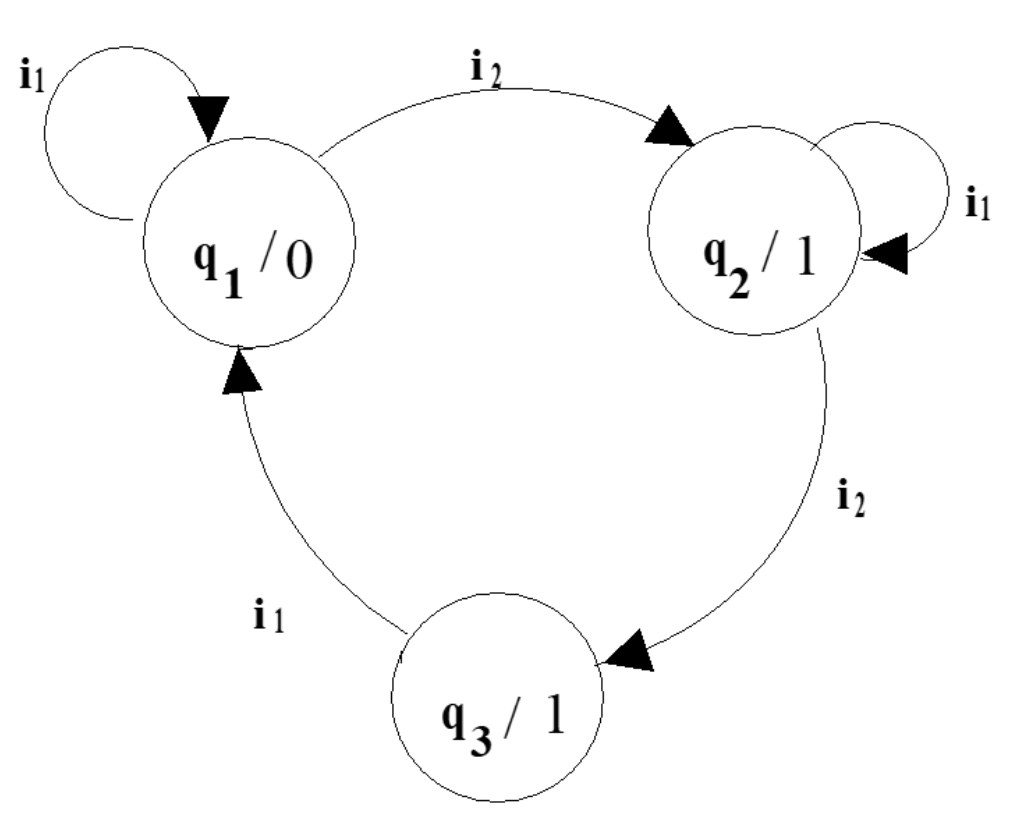
\includegraphics[width=0.35\textwidth]{macchina-moore.png}
    \caption{Macchina di Moore}
    \label{fig:macchina_moore}
\end{figure}

\vspace{1em}
\noindent
Esiste anche la rappresentazione tramite un \textbf{grafo} (o \textbf{diagramma degli stati}) secondo \textbf{Mealy}, in cui
\begin{itemize}
    \item le uscite dipendono dagli stati e dagli ingressi;
    \item in base al valore di ingresso ed allo stato attuale si definisce lo stato futuro e ovviamente l'uscita.
\end{itemize}

\begin{figure}[H]
    \centering
    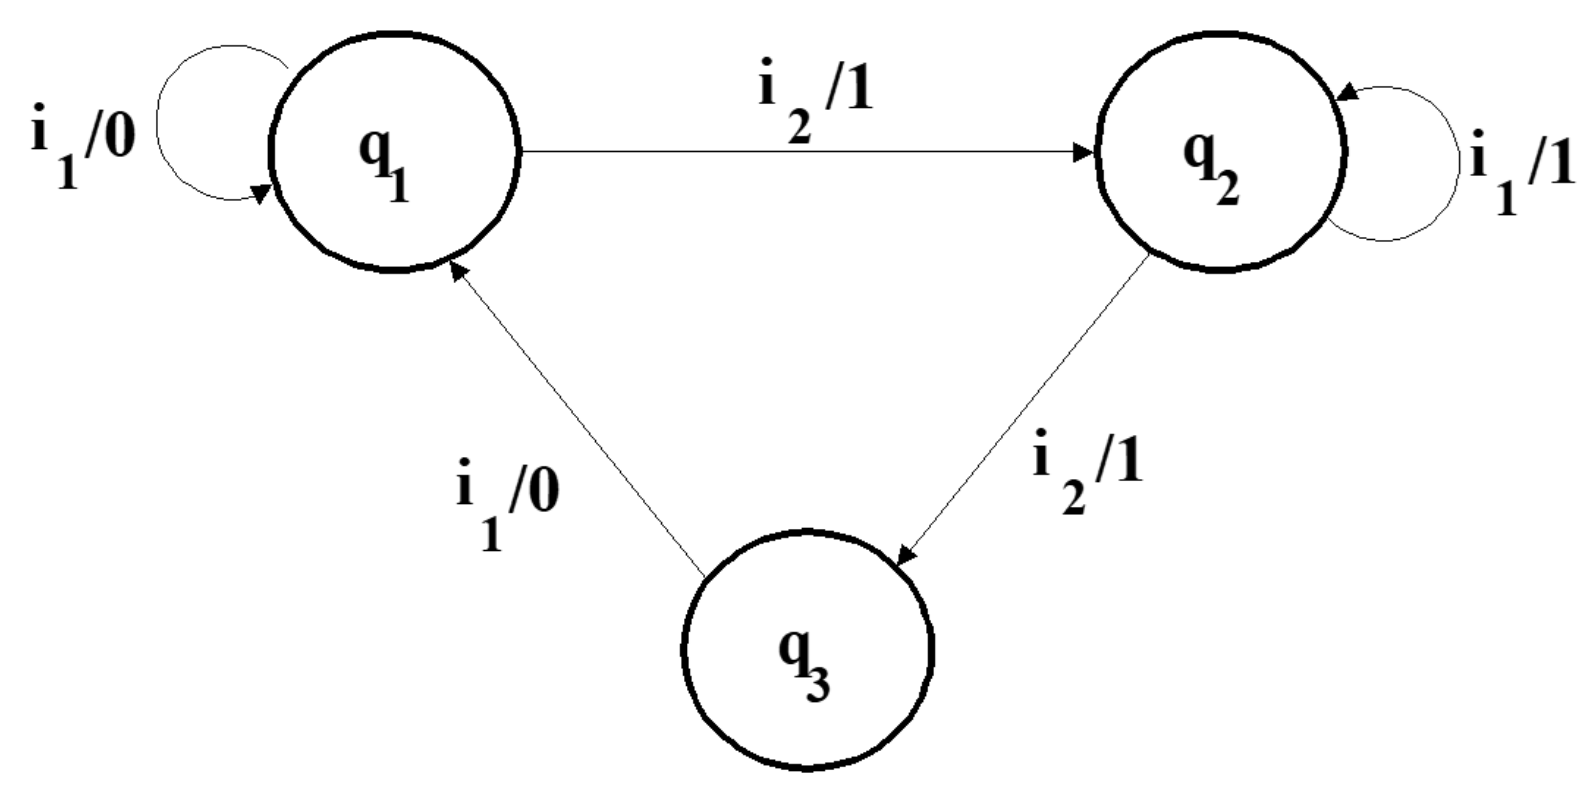
\includegraphics[width=0.45\textwidth]{macchina-mealy.png}
    \caption{Macchina di Mealy}
    \label{fig:macchina_mealy}
\end{figure}

\vspace{1em}
\noindent
Pertanto nella macchina di Moore l'uscita dipende solo dallo stato, mentre nella macchina di Mealy, oltre che dallo stato, l'uscita dipende anche dall'ingresso, il quale modifica l'evoluzione della macchina.

\vspace{1em}
\noindent
\subsection{Equivalenza delle rappresentazioni}
È possibile anche rappresentare una macchina a stati finiti tramite la tavola di Huffman, sempre secondo i modelli di Moore o Mealy.\\
Ogni macchina può essere rappresentata tanto tramite Moore quanto tramite Mealy e si può passare agevolmente dall'una all'altra rappresentazione.

\vspace{1em}
\noindent
\subsubsection{Passaggio da Moore a Mealy}
Per passare da Moore a Mealy, si procede tramite
\begin{itemize}
    \item l'eliminazione dell'uscita dai nodi;
    \item l'associazione della relativa uscita a tutti i rami entranti nel nodo.
\end{itemize}

\begin{figure}[H]
    \centering
    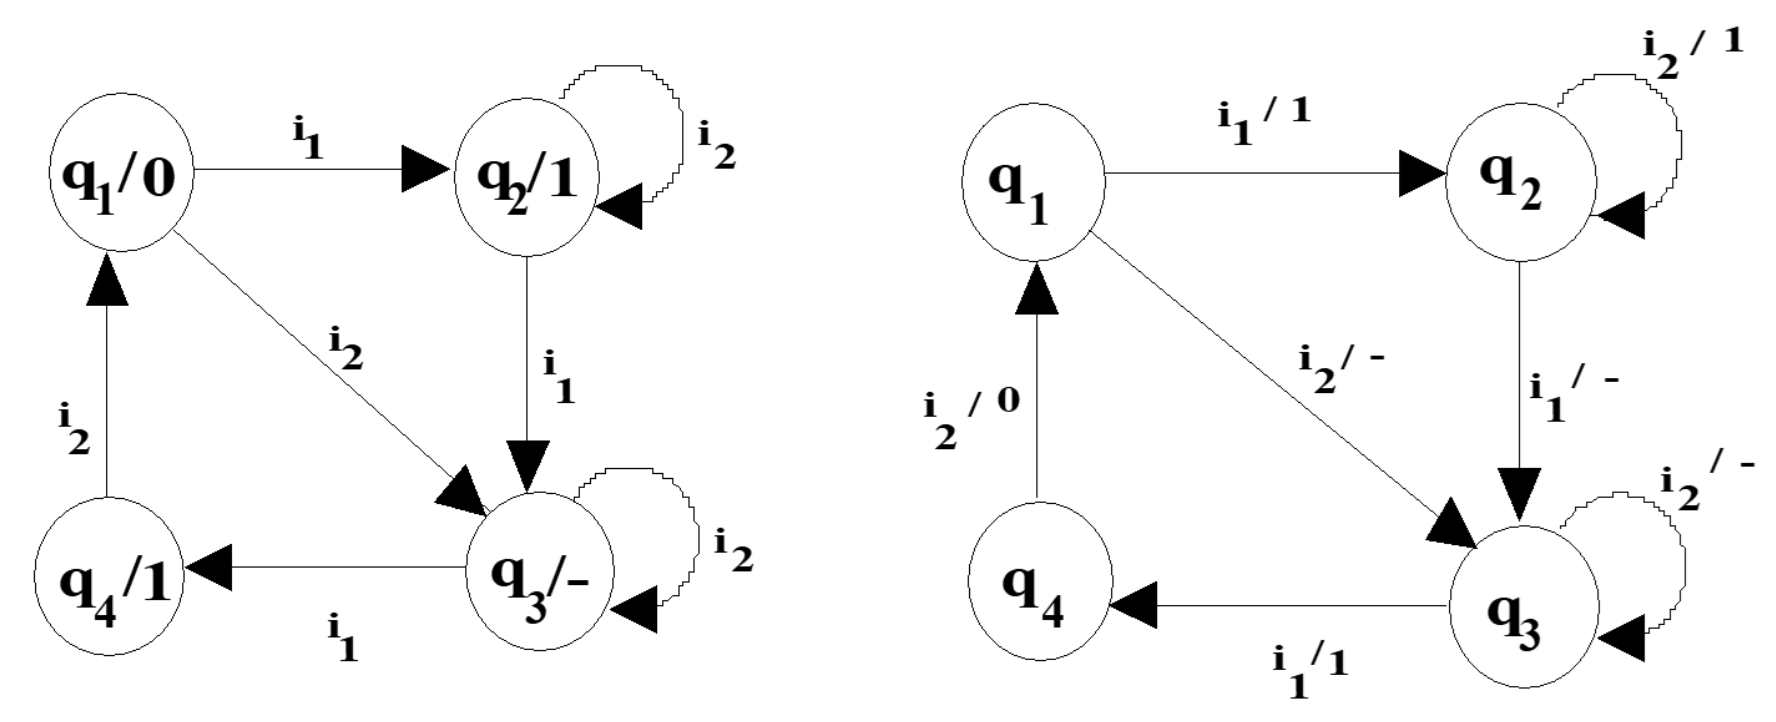
\includegraphics[width=0.55\textwidth]{passaggio-moore-mealy.png}
    \caption{Passaggio da Moore a Mealy}
    \label{fig:passaggio_moore_mealy}
\end{figure}

\vspace{1em}
\noindent
\subsubsection{Passaggio da Mealy a Moore}
Il passaggio da Mealy a Moore può richiedere l'aggiunta di nodi (tanti quanti sono gli stati raggiunti
con uscite differenti), come mostrato nel seguito:

\noindent
\begin{figure}[H]
    \begin{subfigure}{0.5\textwidth}
        \centering
        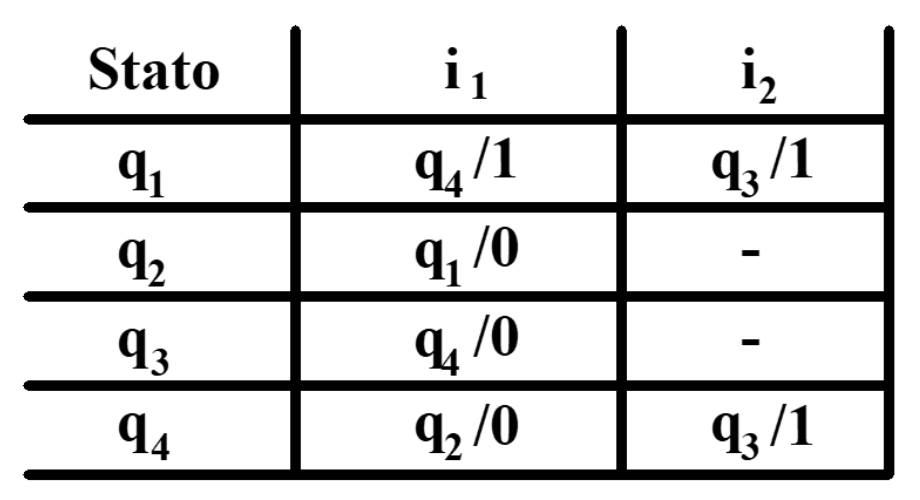
\includegraphics[width=1\textwidth]{passaggio-mealy-moore-1.png}
    \end{subfigure}
    \begin{subfigure}{0.4\textwidth}
        \centering
        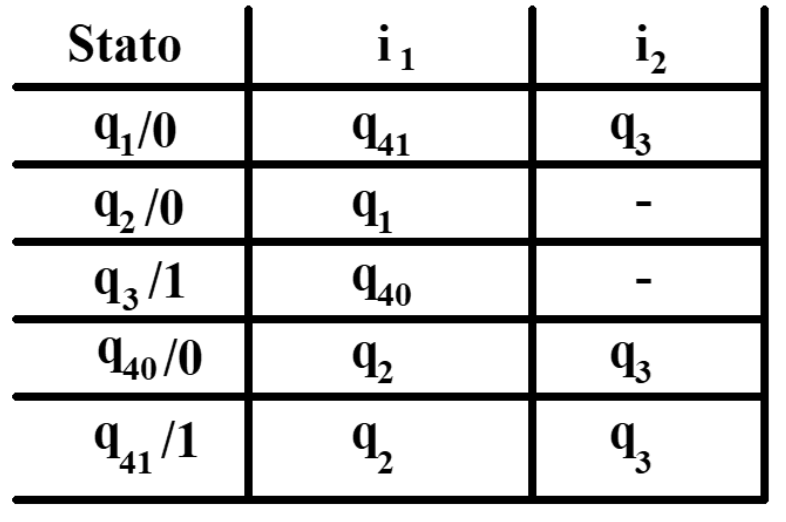
\includegraphics[width=1\textwidth]{passaggio-mealy-moore-2.png}
    \end{subfigure}
    \caption{Passaggio da Mealy a Moore}
    \label{fig:passaggio_mealy_moore}
\end{figure}

\vspace{1em}
\noindent
in cui, ovviamente, mentre $q_3$ comporta sempre l'uscita $1$, mentre $q_4$ deve venir sdoppiato.

\vspace{1em}
\noindent
\textbf{Esempio}: I grafi spesso vengono ottenuti da una descrizione verbale. Per esempio, si realizzi la macchina che rappresenti il risultato di una somma binaria a più bit, sapendo che i bit vengano forniti sequenzialmente dal meno significativo al più significativo:
\begin{itemize}
    \item siccome li stati mantengano memoria del riporto al passo precedente, secondo il modello di Mealy bastano $2$ stati: riporto$=1$ o riporto$=0$
    
    \begin{figure}[H]
        \centering
        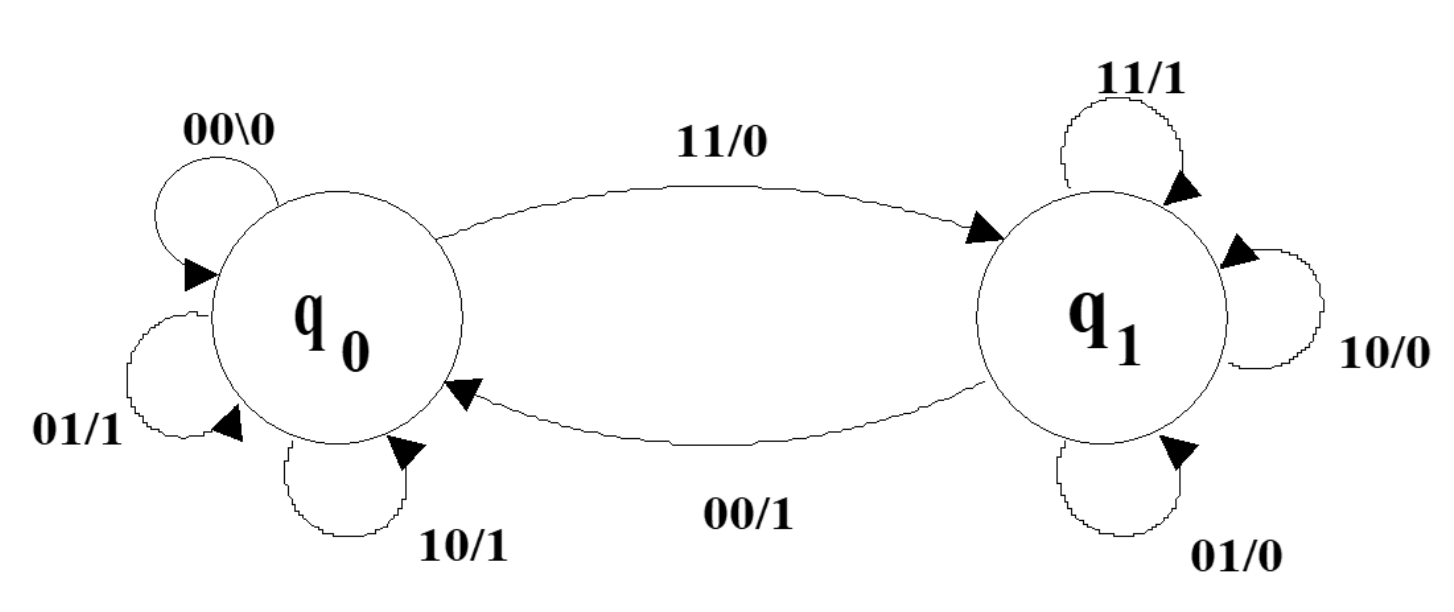
\includegraphics[width=0.55\textwidth]{sommatore-2-bit-mealy.png}
        \caption{Sommatore secondo Mealy}
        \label{fig:sommatore_mealy}
    \end{figure}
    
    \item il modello secondo Moore è più complesso, in quanto si deve differenziare tra gli stati in cui l'uscita è $1$ o $0$ in base al riporto precedente
    
    \begin{figure}[H]
        \centering
        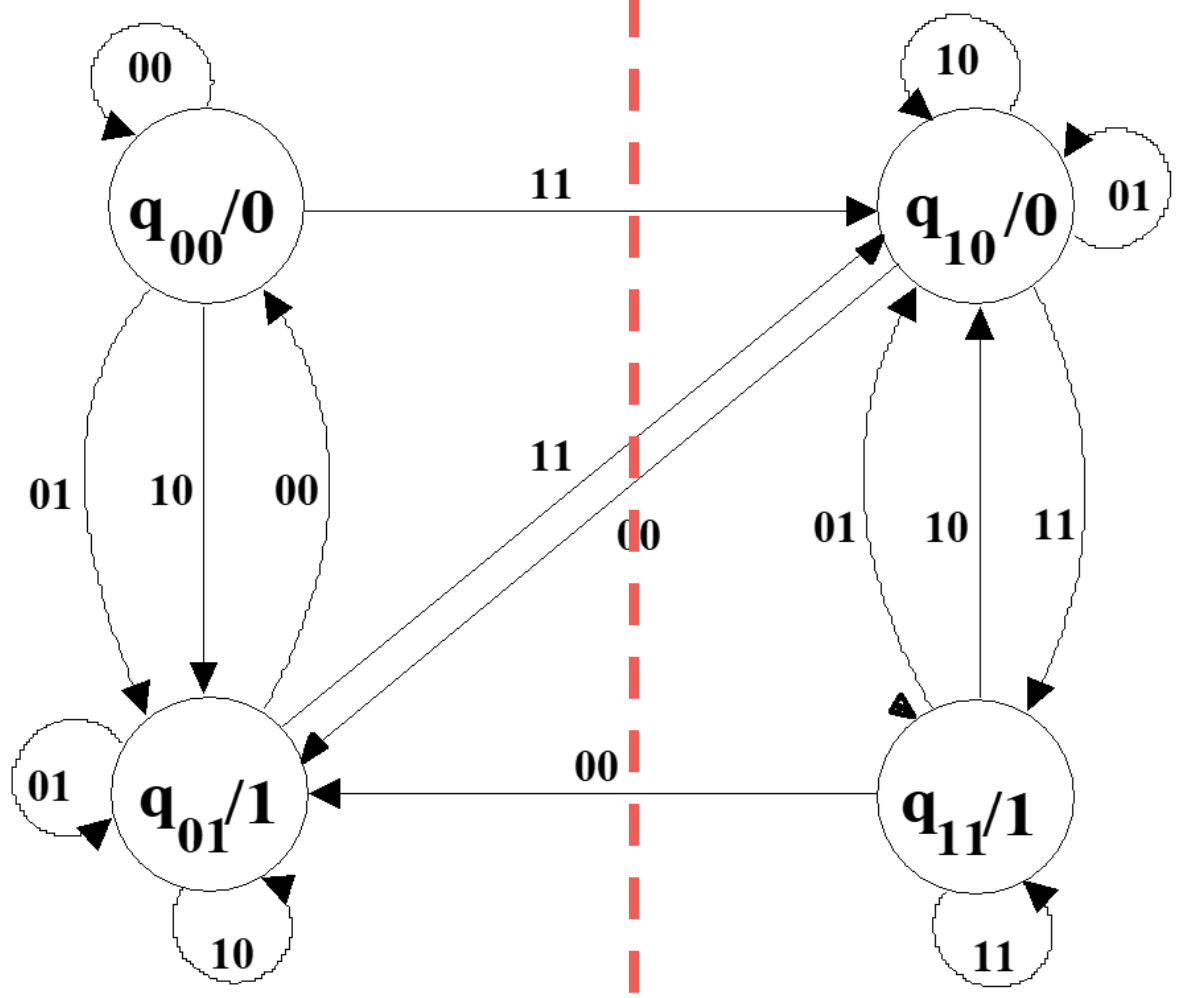
\includegraphics[width=0.55\textwidth]{sommatore-2-bit-moore.png}
        \caption{Sommatore secondo Moore}
        \label{fig:sommatore_moore}
    \end{figure}
\end{itemize}

\vspace{1em}
\subsection{Macchine e stati}
Si forniscono di seguito alcune importanti definizioni:
\begin{itemize}
    \item \textbf{Stato stabile}: se ogni ingresso che porta la macchina in $q_j$ mantiene la macchina in $q_j$;
    \item \textbf{Stato instabile}: se esiste un ingresso che porta la macchina in $q$ e poi la fa evolvere verso un altro stato;
    \item \textbf{Macchina asincrona}: se essa basa il suo funzionamento solo su stati stabili;
    \item \textbf{Macchina sincrona}: se essa effettua delle transizioni che sono sincronizzate tramite un sistema di supervisione, chiamato \textbf{clock};
    \item \textbf{Sequenza applicabile}: la sequenza
    \[i_1,i_2,\dots,i_n\]
    si dice applicabile alla macchina $M$ nello stato $q$ se per ogni ingresso della sequenza esiste lo stato corrispondente $q_i$ e se è definita l'uscita finale $W(q_n,i_n)$.\\
    In una macchina completa tutte le sequenze sono applicabili, in quanto per ogni stato $q_i$ è definita la commutazione allo stato successivo in corrispondenza di ogni possibile ingresso.
    \item \textbf{Macchina equivalente}: una macchina sequenziale $M'$ si dice equivalente a una macchina sequenziale $M$ se tutte le sequenze di ingresso $\sigma_i$ applicabili ad uno stato $q$ di $M$ sono applicabili ad uno stato $q'$ di $M'$ e producono la stessa uscita finale $w' = w$, qualsiasi sia $\sigma_i$.\\
    Attenzione che per le macchine equivalenti non vale le proprietà di simmetria (come, per esempio, nel caso di uscite non definite);
    \item \textbf{Macchina minima}: è una macchina equivalente col minimo numero di stati.
\end{itemize}

\vspace{1em}
\noindent
\textbf{Osservazione}: Si noti che, invece, che una macchina asincrona modifica il proprio stato solo in conseguenza ad una variazione degli ingressi.\\
Chiaramente, però, una macchina asincrona deve potersi fermare in degli stati stabili, altrimenti si avrebbe una continua commutazione dello stato, senza un controllo sulla loro frequenza.\\
Non solo, ma un'altra importante condizione necessaria per il funzionamento di una macchina asincrona è mantenere l'ingresso costante fino a che non avviene una commutazione di stato: se l'ingresso viene modificato prima della commutazione di stato, la macchina avrà un'evoluzione non definita.

\newpage
\begin{center}
    22 Novembre 2022
\end{center}
Shift-Register

\newpage
\begin{center}
    24 Novembre 2022
\end{center}
Per quanto già noto, si ha che
\begin{itemize}
    \item Nei circuiti combinatori
    \begin{itemize}
        \item l'uscita dipende solo dagli ingressi;
        \item la variabile temporale non appare esplicitamente.
    \end{itemize}
    \item Nei circuiti sequenziali
    \begin{itemize}
        \item l'uscita dipende dalla storia passata;
        \item deve esistere una \quotes{memoria} della storia passata.
    \end{itemize}
\end{itemize}

\vspace{1em}
\subsection{Flip-Flop set-reset}
Un flip-flop è un circuito bistabile
\begin{itemize}
    \item con gli ingressi a $0$ sono possibili $2$ stati di equilibrio, ossia $x=0$ e $y=1$ oppure $x=1$ e $y=0$; quindi l'uscita $x=0$ e $y=0$ oppure $x=1$ e $y=1$ non sono stabili;
    \item un impulso su $s$ (set) pone $y=1$ e $x=0$;
    \item un impulso su $c$ (clear) pone $y=0$ e $x=1$;
    \item un impulso sia su $c$ che su $s$ NON è previsto porterebbe le uscite $x=0$ ed $y=0$ dalla quale l'evoluzione è incerta.
\end{itemize}
Si ottiene, quindi, la schematizzazione seguente:

\begin{figure}[H]
    \centering
    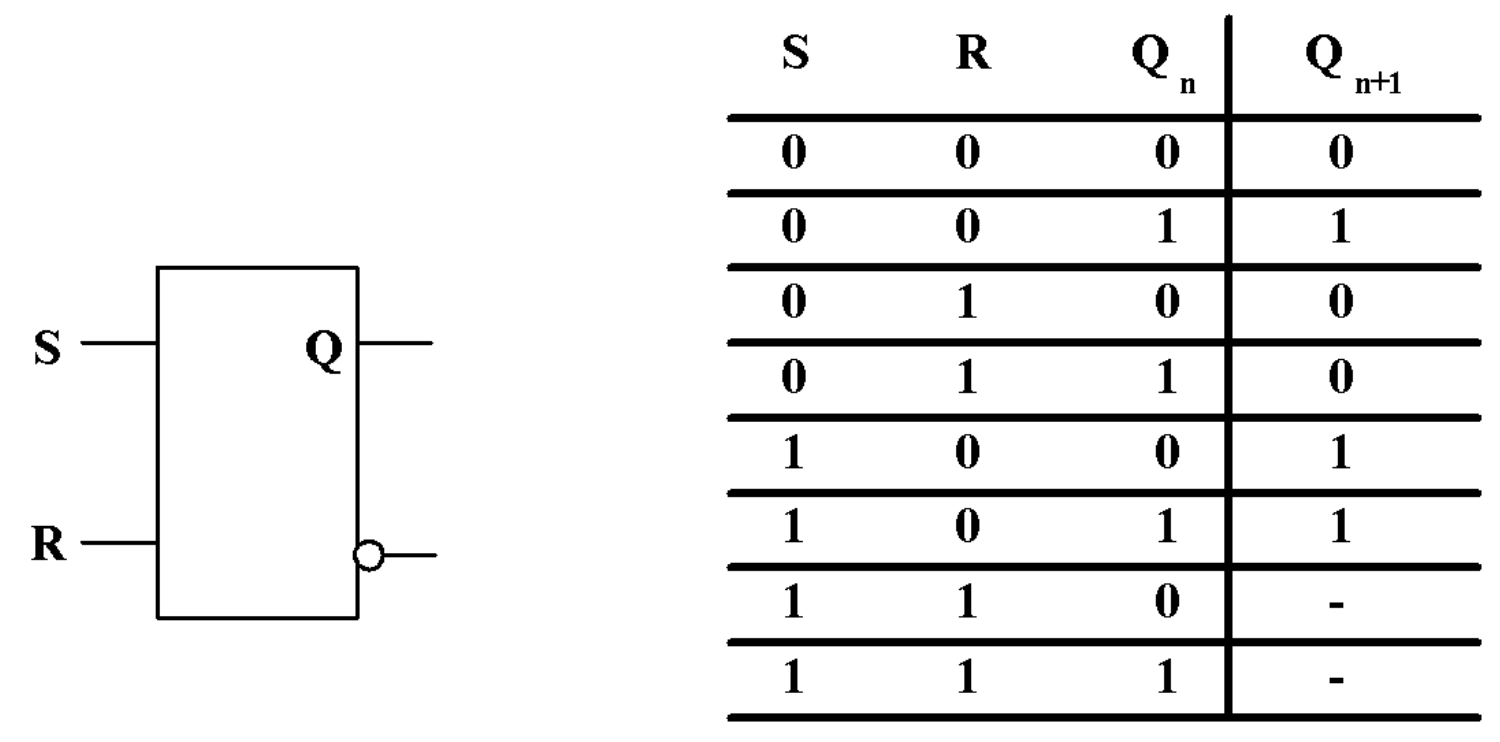
\includegraphics[width=0.5\textwidth]{flip-flop-set-reset.png}
    \caption{Flip-Flop set reset}
    \label{fig:flip-flop-set-reset}
\end{figure}

\vspace{1em}
\noindent
in cui si ha che
\[Q_{n+1} = S + Q_n \cdot \overline{R}\]
con il vincolo che
\[S \cdot R = 0\]

\vspace{1em}
\subsection{Circuiti sincronizzati}
In quasi tutti i circuiti sequenziali le commutazioni avvengono solo in precisi istanti di campionamento, pertanto
\begin{itemize}
    \item vi è la presenza di un segnale di sincronizzazione (Clock);
    \item la loro realizzazione risulta semplificata
    \item il loro funzionamento risulta più affidabile
\end{itemize}
Quindi un circuito sequenziale sincronizzato da un impulso di clock può cambiare stato solo in corrispondenza di tale impulso e cambierà stato non più di una volta per ciascun impulso di clock.

\vspace{1em}
\subsection{Flip-Flop JK}
Il flip-flop JK è più comune del flip-flop set-reset perché prevede anche la possibilità che entrambi gli ingressi siano alti (in tal caso di ha la commutazione di stato).\\
Si ottiene, quindi, la schematizzazione seguente:

\begin{figure}[H]
    \centering
    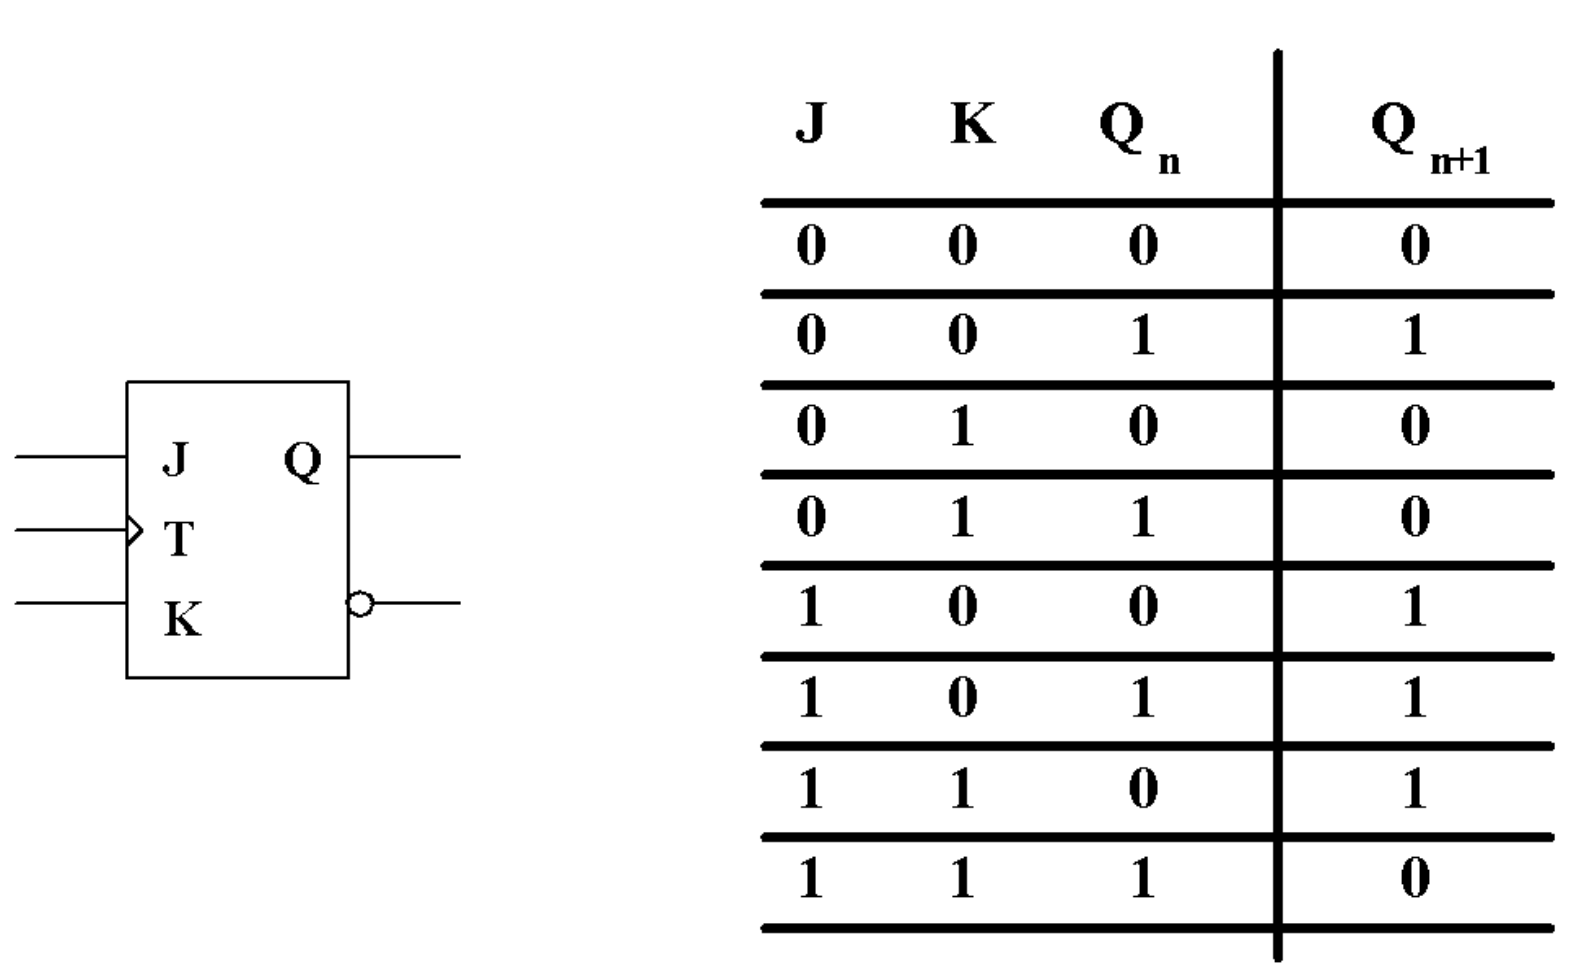
\includegraphics[width=0.5\textwidth]{flip-flop-jk.png}
    \caption{Flip-Flop JK}
    \label{fig:flip-flop-jk}
\end{figure}

\vspace{1em}
\noindent
in cui si ha che
\[Q_{n+1} = \overline{K} \cdot Q_n + J \cdot \overline{Q_n}\]
con il vincolo che
\[S \cdot R = 0\]

\vspace{1em}
\subsection{Flip-Flop T (Toggle)}
Il flip-flop T (Toggle) è un flip-flop che ad ogni impulso di clock cambia di stato, ovvero
\[Q_{n+1} = \overline{Q_n}\]
Esso possiede due ingressi, denominati $T$ e $clk$, in cui ad ogni impulso di clock, se $T=1$ l'uscita commuta di stato
\[Q_{n+1} = Q_n \cdot \overline{T_n} + \overline{Q_n} \cdot T_n = Q_n \oplus T_n\]
che, quindi, può essere ottenuto partendo da un flip-flop JK con entrambi gli ingressi posti in parallelo (ottenendo l'ingresso $T$).

\vspace{1em}
\subsection{Flip-Flop D (Delay)}
Un flip-flop D (Delay) è un flip-flop in cui, ad ogni impulso di clock l'uscita prende il valore presente sull'ingresso $D$
\[Q_{n+1}=D_n\]
e, quindi, può essere realizzato a partire da un flip-flop JK portando sui piedini $J$ e $K$ due segnali che siano uno il negato dell'altro.

\newpage
\noindent
\subsection{Modello generale per i circuiti sequenziali}
In un circuito sequenziale generale 

\begin{figure}[H]
    \centering
    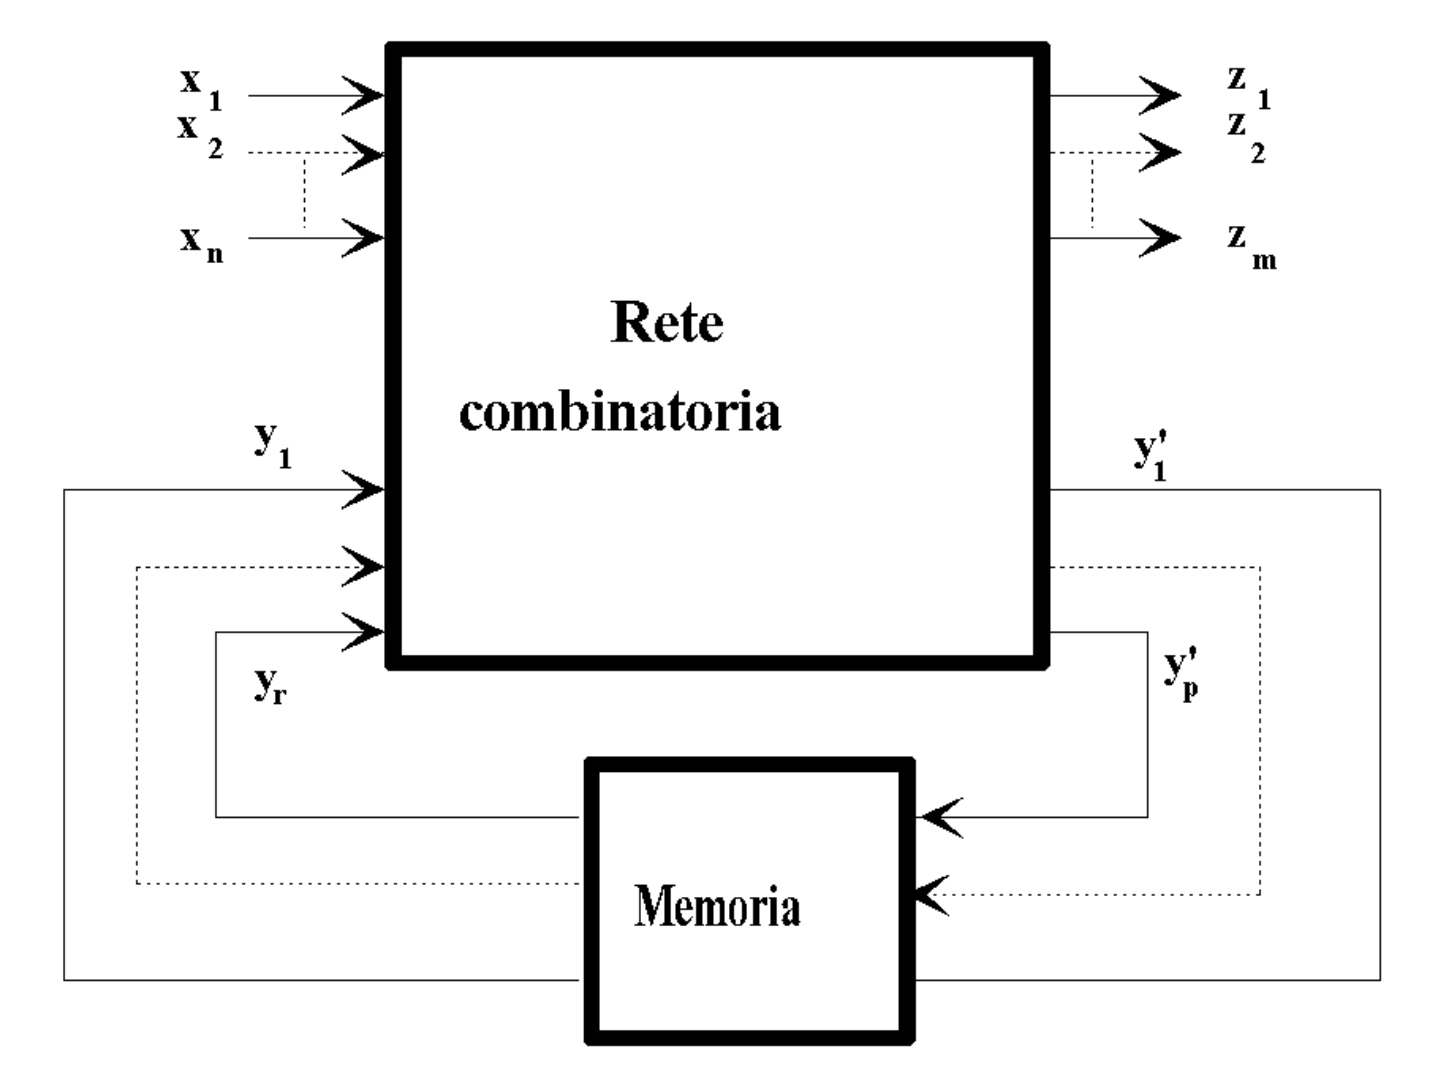
\includegraphics[width=0.5\textwidth]{modello-generale-circuiti-sequenziali.png}
    \caption{Modello generale per i circuiti sequenziali}
    \label{fig:modello_generale_circuiti_sequenziali}
\end{figure}

\noindent
vi è una memoria che mantiene l'informazione dello stato, il quale è rappresentato dalle $2^r$ possibili combinazioni delle variabili $y$.\\
L'uscita dipende dagli ingressi e dallo stato e le variabili di eccitazione $y'$ sono legate a $y$ in base al tipo di memoria: ad esempio potrebbero essere $r=p$ e
\[y(t+\Delta)=y'(t)\]
pertanto lo stato futuro dipende dagli ingressi e dallo stato attuale.

\vspace{1em}
\subsubsection{Funzionamento sincrono}
Nel funzionamento asincrono la memoria è solo un mero ritardo temporale. Nel funzionamento sincrono, invece, la memoria è sincronizzata su un clock, per cui
\begin{itemize}
    \item lo stato e gli ingressi (della memoria) possono variare solo in istanti equi-intervallati, dettati dal clock;
    \item non vi è più di una commutazione per ogni impulso di clock;
    \item il clock deve essere sufficientemente breve da evitare al loop di chiudersi;
    \item le uscite e le variabili di eccitazione sono a \quotes{livelli};
    \item durante il clock le variabili di eccitazione siano stabili
    \item li istanti di clock siano 
    \[t_n \hspace{1em} \text{con} \hspace{1em} n=1,2,\dots\]
    Non solo, ad ogni clock si ha che lo stato si modifica, ovvero
    \[y_n \to y_{n+1} = f(y'_n)\]
    Ovviamente, però, le variabili di uscita e di eccitazione si modificano e si stabilizzano prima dell'arrivo del nuovo clock.
\end{itemize}

\vspace{1em}
\subsection{Protocollo IIC (I2C o I$^2$C)}
Il protocollo IIC è un protocollo di comunicazione sviluppato dalla Philips che permette a Master e Slave di comunicare fra loro impiegando due soli fili di collegamento: SCL, per la sincronizzazione tra Master e Slave, e SDA per la trasmissione dei dati.\\
Ovviamente, dovendo comunicare su uno stesso bus di comunicazione, Master e Slave devono potersi scollegare dal bus, per cui vi sono $3$ stati per ognuno
\begin{itemize}
    \item stato $1$: bus libero;
    \item stato $0$: bus occupato;
    \item stato $z$: alta impedenza, Master/Slave scollegato.
\end{itemize}
Il bus è libero quando sia SCL che SDA sono entrambi alti, al livello $1$; quando si vuole comunicare, si abbassa prima il segnale SDA e poi SCL: pertanto la sequenza SDA-SCL$=11-01$ dà inizio alla trasmissione.\\
Iniziata la comunicazione, quando si vuole trasmettere si deve impostare il segnale SDA (al livello $1$ o $0$) e dare un colpo di SCL (sempre a $1$); alla fine della trasmissione si riportano SCL e SDA al livello alto, ma prima SCL e poi SDA questa volta: pertanto la sequenza SDA-SCL$=01-11$ finisce la trasmissione.\\
Pertanto l'inizio e la fine della trasmissione sono gli unici casi in cui SDA presenta un fronte di salita/discesa quando SCL è alto: in particolare
\begin{itemize}
    \item quando SCL è alto e SDA passa da $1$ a $0$ inizia la trasmissione;
    \item quando SCL è alto e SDA passa da $0$ a $1$ finisce la trasmissione;
\end{itemize}
Descrivendo tale macchina a stati tramite la tavola di Haffmann si ottiene

\vspace{1em}
\noindent
\begin{table}[H]
    \rowcolors{1}{white}{white}
\setlength{\tabcolsep}{4pt}
\renewcommand{\arraystretch}{1.2}
\centering
\begin{tabular}{c|cccc|cl}
        & $00$ & $01$ & $11$ & $10$ & & \\
    \hline
    $A$ & $-$         & $-$          & $B$          & $-$         & $0$ & Stop\\ 
    $B$ & $-$         & $C$          & $\boxed{B}$  & $-$         & $0$ & \\
    $C$ & $D$         & $\boxed{C}$  & $-$          & $-$         & $1$ & Start\\
    $D$ & $\boxed{D}$ & $E$          & $\boxed{D}$  & $\boxed{D}$ & $1$ & Trasmissione\\
    $E$ & $D$         & $\boxed{D}$  & $A$          & $-$         & $1$ & Preallarme\\
\end{tabular}
\end{table}

\vspace{1em}
\noindent
Applicando il metodo di Ginsburg per è immediato evincere che $A$ e $B$ sono praticamente lo stesso stato. Procedendo con la semplificazione si ottiene

\vspace{1em}
\noindent
\begin{table}[H]
    \rowcolors{1}{white}{white}
\setlength{\tabcolsep}{4pt}
\renewcommand{\arraystretch}{1.2}
\centering
\begin{tabular}{c|c|c|c|c}
    $CD$ & $D$ & $CE$ & $D$ & $D$\\
    \hline
    $CE$ & $D$ & $CE$ & $A$ & $-$\\
    \hline
    $DE$ & $D$ & $E$ & $DA$ & $D$
\end{tabular}
\end{table}

\noindent
In cui appare evidente che l'accoppiamento $DE$ non è più possibile. Si possono quindi realizzare $3$ stati: $AB$, $CE$ e $D$, oppure $AB$, $CD$ ed $E$. Si sceglie la prima terna, per cui si ha che

\vspace{1em}
\noindent
\begin{table}[H]
    \rowcolors{1}{white}{white}
\setlength{\tabcolsep}{4pt}
\renewcommand{\arraystretch}{1.2}
\centering
\begin{tabular}{c|c|c|c|c|cl}
         & $00$ & $01$ & $11$ & $10$\\
    $AB$ & $-$  & $CE$ & $AB$ & $-$ & $0$ & Stop\\
    \hline
    $CE$ & $D$  & $CE$ & $AB$ & $-$ & $1$ & Start/Preallarme\\
    \hline
    $D$  & $D$  & $CE$ & $D$ & $D$ & $1$ & Trasmissione
\end{tabular}
\end{table}

\vspace{1em}
\noindent
Per la rappresentazione della macchina a stati semplificata, è fondamentale codificare opportunamente gli stati con una codifica binaria che deve rispettare il fatto che due stati contigui non devono mai essere codificati con due valori binari in cui commutano due bit contemporaneamente.

\newpage
\begin{center}
    29 Novembre 2022
\end{center}
Un circuito sequenziale asincrono è una logica combinatoria che presenta degli ingressi e degli stati iniziali: in funzione dello stato corrente e degli ingressi, la logica fornisce l'uscita desiderata e gli stati futuri, i quali verranno retro-azionati in ingresso.\\
Da notare che uno stato è stabile se data una configurazione di stati iniziali, in funzione di certi ingressi producono in uscita gli stessi stati, che retro-azionati in ingresso continuano a produrre il medesimo stato.

\vspace{1em}
\noindent
\subsection{Analisi di circuiti sequenziali asincroni}
Power-Point 6\\
Il modello semplificato adottato prevede che tutti i ritardi sono i medesimi.\\
Si provi a studiare, ora, il Latch di NOR, realizzato come segue


\vspace{1em}
\noindent
in cui la porta NOR funziona come un invertitore controllato: se uno dei due ingressi è a $0$, allora funziona come invertitore, altrimenti se l'ingresso è a $1$ in uscita si avrà sempre $0$.\\
I loop di reazione, in questo caso, sono solo $1$, e non due come si potrebbe pensare. Si concentri, allora, tutto il ritardo $\Delta$ sull'unico loop di reazione.\\
In particolare, è facile capire
\[Y'=\overline{\overline{S+Y}+R} = (S+Y) \cdot \overline{R}\]
mentre si ottiene che
\[Z_1=\overline{S+Y} \hspace{1em} \text{e} \hspace{1em} Z_2=Y'\]
Allora si scrivano in una mappa di Karnaugh le funzioni così ottenute $Y'$, $Z_1$ e $Z_2$, individuando gli implicanti in modo inverso.

\vspace{1em}
\noindent
Mettendo insieme le due tabelle, si ottiene il funzionamento del circuito secondo una macchina di Mealy:

\vspace{1em}
\noindent
È facile capire quali sono gli stati stabili: leggendo per righe la tabella, dove $Y$ ha valore $0$, tutti gli stati che producono come uscita $0$ sono stabili, in quanto lo $0$ viene retro-azionato; similmente per $Y=1$.

\vspace{2em}
\noindent
\textbf{Esempio}: Nell'esempio descritto di seguito

\vspace{1em}
\noindent
si individuano due loop di reazione; per ognuno di essi si descrive l'espressione esatta
\[Y_1'=Y_1X + Y_2 \overline{X} \hspace{1em} \text{e} \hspace{1em} Y_2'=\overline{Y_1}X + Y_2 \overline{X}\]
Ancora una volta si rappresentano $Y_1'$ e $Y_2'$ in opportune mappe di Karnaugh, individuando gli implicanti al contrario:

\vspace{1em}
\noindent
Mettendo insieme le due tabelle, è facile capire quali sono gli stati stabili.\\
Da notare, poi, che non esiste differenza tra $Y_1$ e $Y_1'$, così come $Y_2$ e $Y_2'$, in quanto il ritardo non è concentrato nei loop di reazione, come si fa nella semplificazione.\\
Infatti, scegliendo come uscita $Y_2$ o $Y_2'$ cambiano solamente le uscite riportate negli stati instabili, mentre quelle degli stati rimangono le medesime, ed è quello che conta.











\end{document}
